% Template source: https://www.overleaf.com/project/5c3f179666c6b83e735fb136

% Font size: 12pt
% Format A4 paper
% Openright: open chapters on the right
% Twoside: front and back document
% Report: thesis style (or book)
\documentclass[12pt,a4paper,openright,twoside]{report}
\usepackage[italian]{babel} % Italian dictionary library
\usepackage[T1]{fontenc}
\usepackage[utf8]{inputenc} % Italian characters
\usepackage{fancyhdr} % Document layout library
\usepackage{indentfirst} % Indentation at the beginning of the chapters
%\usepackage{showkeys} % Label's library
\usepackage{graphicx} % Graph's library
\graphicspath{{assets/images}}
\usepackage{newlfont} % Custom fonts library
% Math libraries
\usepackage{amssymb}
\usepackage{amsmath}
\usepackage{latexsym}
\usepackage{amsthm}
\usepackage{listings}
\usepackage{hyperref}
\usepackage[square,numbers,sort]{natbib}
\usepackage{xcolor}
\usepackage{colortbl}
\usepackage{array}
\usepackage{adjustbox}
\usepackage{tikz}
\usepackage{tikz-3dplot}
\usepackage{float}
\usepackage{fancyvrb}
\usepackage{subcaption}
\usepackage[acronym, automake]{glossaries}
\makeglossaries
% In alphabetical order
\newacronym{acid}{ACID}{Atomicity, Consistency, Isolation and Durability}
\newacronym{ajax}{AJAX}{Asynchronous JavaScript and XML}
\newacronym{api}{API}{Application Programming Interface}
\newacronym{aqi}{AQI}{Air Quality Index}
\newacronym{bson}{BSON}{Binary JSON}
\newacronym{cap}{CAP}{Codice Avviamento Postale}
\newacronym{cli}{CLI}{Command Line Interface}
\newacronym{co}{CO}{Monossido di carbonio}
\newacronym{cqrs}{CQRS}{Command Query Responsibility Segregation}
\newacronym{crs}{CRS}{Coordinate Reference Systems}
\newacronym{css}{CSS}{Cascading Style Sheets}
\newacronym{csv}{CSV}{Comma Separated Values}
\newacronym{dom}{DOM}{Document Object Model}
\newacronym{eaqi}{EAQI}{European Air Quality Index}
\newacronym{eea}{EEA}{European Environment Agency}
\newacronym{epsg}{EPSG}{European Petroleum Survey Group}
\newacronym{gis}{GIS}{Geographic Information System}
\newacronym{gps}{GPS}{Global Positioning System}
\newacronym{html}{HTML}{HyperText Markup Language}
\newacronym{iogp}{IOGP}{International Association of Oil \& Gas Producers}
\newacronym{iot}{IOT}{Internet of Things}
\newacronym{iqa}{IQA}{Indice di Qualità dell'Aria}
\newacronym{json}{JSON}{Javascript Object Notation}
\newacronym{lifo}{LIFO}{Last In First Out}
\newacronym{no2}{NO2}{Diossido di azoto}
\newacronym{npm}{npm}{Node Package Manager}
\newacronym{o3}{O3}{Ozono}
\newacronym{osm}{OSM}{OpenStreetMap}
\newacronym{pm10}{PM10}{Particolato PM10}
\newacronym{pm25}{PM2.5}{Particolato PM2.5}
\newacronym{pwa}{PWA}{Progressive Web App}
\newacronym{pypi}{PyPI}{Python Package Index}
\newacronym{ql}{QL}{Query Language}
\newacronym{rest}{REST}{Representational State Transfer}
\newacronym{sfc}{SFC}{Single File Components}
\newacronym{so2}{SO2}{Anidride solforosa}
\newacronym{spa}{SPA}{Single Page Applications}
\newacronym{srp}{SRP}{Single Responsibility Principle}
\newacronym{svg}{SVG}{Scalable Vector Graphics}
\newacronym{ttl}{TTL}{Time To Live}
\newacronym{wgs84}{WGS84}{World Geodetic System 1984}
\newacronym{xml}{XML}{Extensible Markup Language}
\newacronym{ztl}{ZTL}{Zona Traffico Limitato}

\setlength{\headheight}{14.49998pt}
\addtolength{\topmargin}{-2.49998pt}

% List of IQA colors for table
\definecolor{good}{RGB}{80,240,230}           % Turquoise
\definecolor{fair}{RGB}{80,204,170}           % Aqua green
\definecolor{moderate}{RGB}{240,230,65}       % Yellow
\definecolor{poor}{RGB}{255,80,80}            % Red
\definecolor{verypoor}{RGB}{150,0,50}         % Dark purple
\definecolor{extremelypoor}{RGB}{125,33,129}  % Indigo

\lstset{
  frame=single,   % Adds a frame (border) around code blocks
                  % single means it will be a continuous line that completely surrounds the code
  breaklines=true,% Enables automatic line breaking for long lines
                  % When a line of code is too long to fit within the page width, it will be automatically broken and continued on the next line
  numbers=left,
  basicstyle=\ttfamily\small,
}

\oddsidemargin=30pt \evensidemargin=20pt    % Margins
\hyphenation{sil-la-ba-zio-ne pa-ren-te-si} % It serves for hyphenation

% Page layout setup
\pagestyle{fancy}\addtolength{\headwidth}{20pt}
\renewcommand{\chaptermark}[1]{\markboth{\thechapter.\ #1}{}}
\renewcommand{\sectionmark}[1]{\markright{\thesection \ #1}{}}
\rhead[\fancyplain{}{\bfseries\leftmark}]{\fancyplain{}{\bfseries\thepage}}
\cfoot{}
\linespread{1.3} % Line spaceing

%%%%%%%%%%%%%%%%%%%
% Custom commands %
%%%%%%%%%%%%%%%%%%%
\newcommand{\xstudent}{Matteo Zeno Bagli}
\newcommand{\xsupervisor}{Silvia Mirri}
\newcommand{\xcorrelatored}{Giovanni Delnevo}
\newcommand{\xcorrelatoreo}{Kelvin Olaiya}
\newcommand{\xsession}{II}
\newcommand{\xaccademicyear}{2024-2025}
\newcommand{\donotmumberlastpageonleft}{\clearpage{\pagestyle{empty}\cleardoublepage}}

%%%%%%%%%%%%%%%%%%%
% End of Preamble %
% Document start  %
%%%%%%%%%%%%%%%%%%%

\begin{document}

%%%%%%%%%%%%%%%%%%%%%%%%%%%%%%%%%%%%%%%%%%%
% preface start                           %
%                                         %
% title page, table of contents, abstract %
%%%%%%%%%%%%%%%%%%%%%%%%%%%%%%%%%%%%%%%%%%%


%\textwidth=450pt
\oddsidemargin=25pt

\begin{titlepage}
\begin{center}
{
	{\Large{\textsc{Alma Mater Studiorum}}}\\
	{\Large{\textsc{Universit\`a di Bologna}}} \\
	{\textsc{Campus di Cesena}}
	\rule[0.1cm]{14cm}{0.1mm}
	\rule[0.5cm]{14cm}{0.6mm}
	DIPARTIMENTO DI INFORMATICA – SCIENZA E INGEGNERIA
	Corso di Laurea Magistrale in Ingegneria e Scienze Informatiche
}
\end{center}
\vspace{15mm}
\begin{center}
{\LARGE{\bf SIMULATORE DI MISURAZIONI TRAMITE RETE DI SENSORI SULLA QUALITÀ DELL'ARIA: PROGETTO E SVILUPPO}}
\end{center}
\vspace{40mm}
\par
\noindent
\begin{minipage}[t]{0.47\textwidth}
{\large{\bf Relatore:\\Prof.ssa \xsupervisor}}
\vspace{5mm}
{\large{\bf \\Correlatore:\\Dr. \xcorrelatore}}
\end{minipage}
\hfill
\begin{minipage}[t]{0.47\textwidth}\raggedleft
{\large{\bf Presentata da:\\\xstudent}}
\end{minipage}
\vspace{20mm}
\begin{center}
{\large{\bf Sessione \xsession\\Anno Accademico \xaccademicyear}}
\end{center}
\end{titlepage}
\begin{titlepage}
\thispagestyle{empty} % Remove page number
\topmargin=6.5cm      % Set margin top to 6.5cm
\raggedleft           % Align text to the right
\large                % Set font size to 14pt
\em                   % Emphatize (italian style)
A Miriana
\newpage
\clearpage{\pagestyle{empty}\cleardoublepage} % Doesn't number the last left page
\end{titlepage}
%
%%%%%%%%%%%%%%%%%%%%%%%%%%%%%%%%%%%%%%%%
\pagenumbering{roman}                   %serve per mettere i numeri romani
\chapter*{Introduzione}                 %crea l'introduzione (un capitolo
                                        %   non numerato)
%%%%%%%%%%%%%%%%%%%%%%%%%%%%%%%%%%%%%%%%%imposta l'intestazione di pagina
\rhead[\fancyplain{}{\bfseries
INTRODUZIONE}]{\fancyplain{}{\bfseries\thepage}}
\lhead[\fancyplain{}{\bfseries\thepage}]{\fancyplain{}{\bfseries
INTRODUZIONE}}
%%%%%%%%%%%%%%%%%%%%%%%%%%%%%%%%%%%%%%%%%aggiunge la voce Introduzione
                                        %   nell'indice
\addcontentsline{toc}{chapter}{Introduzione}
Questa \`e l'introduzione.
%%%%%%%%%%%%%%%%%%%%%%%%%%%%%%%%%%%%%%%%%non numera l'ultima pagina sinistra
\clearpage{\pagestyle{empty}\cleardoublepage}

\tableofcontents % Index

% Page heading
\rhead[\fancyplain{}{\bfseries\leftmark}]{\fancyplain{}{\bfseries\thepage}}
\lhead[\fancyplain{}{\bfseries\thepage}]{\fancyplain{}{\bfseries INDICE}}

\donotmumberlastpageonleft
\listoffigures % Makes list of figures

\donotmumberlastpageonleft
\listoftables % Makes list of tables

\donotmumberlastpageonleft
\printglossary[type=\acronymtype]

%%%%%%%%%%%%%%%%%%%%%%%%%%%%%%%%%%%%%%%%%%%%%%%%%%%%%%%%%%%%%%%%%%%%%%%%%%%%%%%%%%%%%%%%%
% Document body start                                                                   %
%                                                                                       %
% Sequence of various sections                                                          %
% It is recommended to maintain a well-defined logical structure for section separation %
% It is suggested to reflect this structure physically in the file system               %
%%%%%%%%%%%%%%%%%%%%%%%%%%%%%%%%%%%%%%%%%%%%%%%%%%%%%%%%%%%%%%%%%%%%%%%%%%%%%%%%%%%%%%%%%

% Sections inclusion
\clearpage{\pagestyle{empty}\cleardoublepage}
\chapter{Introduzione del sistema}
\lhead[\fancyplain{}{\bfseries\thepage}]{\fancyplain{}{\bfseries\rightmark}}
\pagenumbering{arabic}

Il primo capitolo ha due obiettivi:
il primo obiettivo è l'introduzione del progetto di tesi, con le sue caratteristiche e funzionalità;
il secondo obiettivo è l'analisi dello stato dell'arte degli attuali sistemi simili al progetto dell'elaborato di tesi,
descrivendone le caratteristiche principali, ponendo i diversi sistemi a confronto e approfondendone le funzionalità.

\section{Scopo del progetto}

Lo scopo del progetto di tesi è quello di presentare un sistema di simulazione atto alla collezione ed interpretazione
di dati sulla qualità dell'aria di una determinata area geografica.

Tali dati provengono da misurazioni fittizie prodotte da sensori distribuiti in un'area di studio.
I sensori inviano tali rilevazioni ad un intermediario, il quale li raccoglie e li rende disponibili.
Viene quindi disposta una dashboard attraverso la quale gli utenti possono fruirne sotto forma di tabelle e
di una mappa interattiva.

La dashboard consiste in una web app mobile-first che permette di visualizzare l'area geografica coinvolta e
i dati sulla qualità dell'aria.
Lo sviluppo della dashboard prende come riferimento le applicazioni della stessa tipologia attualmente presenti
come stato dell'arte.

L'area geografica di interesse è il comune di Bologna, entro il cui perimetro vengono posizionati i sensori
di simulazione.

\cite{Accuweather}

\section{Qualità dell'aria}
I dati sulla qualità dell'aria vengono definiti dai paesi secondo indici e scale.
L'indice di qualità dell'aria (IQA) rappresenta il modo in cui i governi scelgono di comunicare con la popolazione
la qualità dell'aria. Esso converge il livello di diversi inquinanti in un unico indice comprensibile,
consentendo di identificare più facilmente il livello di inquinamento e l'eventuale rischio associato.

Regioni e paesi diversi utilizzano scale differenti per indicare la qualità dell'aria in base all'inquinamento locale e
a considerazioni sulla salute. Esistono decine di indici locali utilizzati in tutto il mondo;
ad esempio, in alcune regioni dell'Australia si utilizzano sistemi basati su numeri, mentre altre ne usano uno basato
su categorie. Canada, Giappone e Stati Uniti definiscono indici di qualità dell'aria distinti, così come
l'Agenzia europea dell'ambiente \cite{EuropeanEnvironmentAgency}.

Il servizio online "The European Air Quality Index" dell'EEA  (European Environment Agency) e
della Commissione Europea fornisce informazioni sulla qualità dell'aria basate su più di 2000 stazioni di rilevamento
in tutta Europa. L'indice consiste in una mappa interattiva che mostra la qualità dell'aria a livello locale,
andando ad analizzare i 5 livelli di inquinanti più pericolosi per le persone e per l'ambiente:

\begin{itemize}
  \item Particolato PM2.5 e PM10
  \item Ozono (O3)
  \item Diossido di azoto (NO2)
  \item Anidride solforosa (SO2)
\end{itemize}

Gli utenti possono zoommare la mappa o ricercare città Europee per controllare la qualità globale dell'aria e verificare i livelli di inquinanti registrati dai sensori dalle stazioni locali. L'Indice mostra un rating globale per ogni stazione di rilevamento, andando a marcare la mappa con un punto colorato, per ognuno dei 5 inquinanti. Il colore indica un livello di qualità dell'aria:
\begin{itemize}
  \item Molto buono (verde acqua)
  \item Buono (verde)
  \item Moderato (giallo)
  \item Basso (rosso)
  \item Molto basso (rosso ciliegia)
  \item Estremamente basso (viola)
\end{itemize}

\begin{table}[h]
  \centering
  \adjustbox{width=\textwidth,center}{
    \begin{tabular}{|>{\raggedright\arraybackslash}m{3cm}|c|c|c|c|c|c|}
      \hline
      \textbf{Inquinante}
       & \textbf{Buono}
       & \textbf{Discreto}
       & \textbf{Moderato}
       & \textbf{Scarso}
       & \textbf{Molto scarso}
       & \textbf{Estremamente scarso}               \\
      \hline
      Particelle inferiori a 2.5 $\mu$m (PM$_{2.5}$)
       & \cellcolor{good}0-5
       & \cellcolor{fair}\color{white}6-15
       & \cellcolor{moderate}16-50
       & \cellcolor{poor}\color{white}51-90
       & \cellcolor{verypoor}\color{white}91-140
       & \cellcolor{extremelypoor}\color{white}>140 \\
      \hline
      Particelle inferiori a 10 $\mu$m (PM$_{10}$)
       & \cellcolor{good}0-15
       & \cellcolor{fair}\color{white}16-45
       & \cellcolor{moderate}46-120
       & \cellcolor{poor}\color{white}121-195
       & \cellcolor{verypoor}\color{white}196-270
       & \cellcolor{extremelypoor}\color{white}>270 \\
      \hline
      Biossido di azoto (NO$_2$)
       & \cellcolor{good}0-06
       & \cellcolor{fair}\color{white}61-100
       & \cellcolor{moderate}101-120
       & \cellcolor{poor}\color{white}121-160
       & \cellcolor{verypoor}\color{white}161-180
       & \cellcolor{extremelypoor}\color{white}>180 \\
      \hline
      Ozono (O$_3$)
       & \cellcolor{good}0-10
       & \cellcolor{fair}\color{white}11-25
       & \cellcolor{moderate}26-60
       & \cellcolor{poor}\color{white}61-100
       & \cellcolor{verypoor}\color{white}101-150
       & \cellcolor{extremelypoor}\color{white}>150 \\
      \hline
      Biossido di zolfo (SO$_2$)
       & \cellcolor{good}0-20
       & \cellcolor{fair}\color{white}21-40
       & \cellcolor{moderate}41-125
       & \cellcolor{poor}\color{white}126-190
       & \cellcolor{verypoor}\color{white}191-275
       & \cellcolor{extremelypoor}\color{white}>275 \\
      \hline
    \end{tabular}
  }
  \caption{Indici di qualità dell'aria per diversi inquinanti secondo l'EEA\cite{EuropeanAirQualityMapAndCharts}}
  \label{tab:air_quality}
\end{table}

% \begin{figure}
%   \centering
%   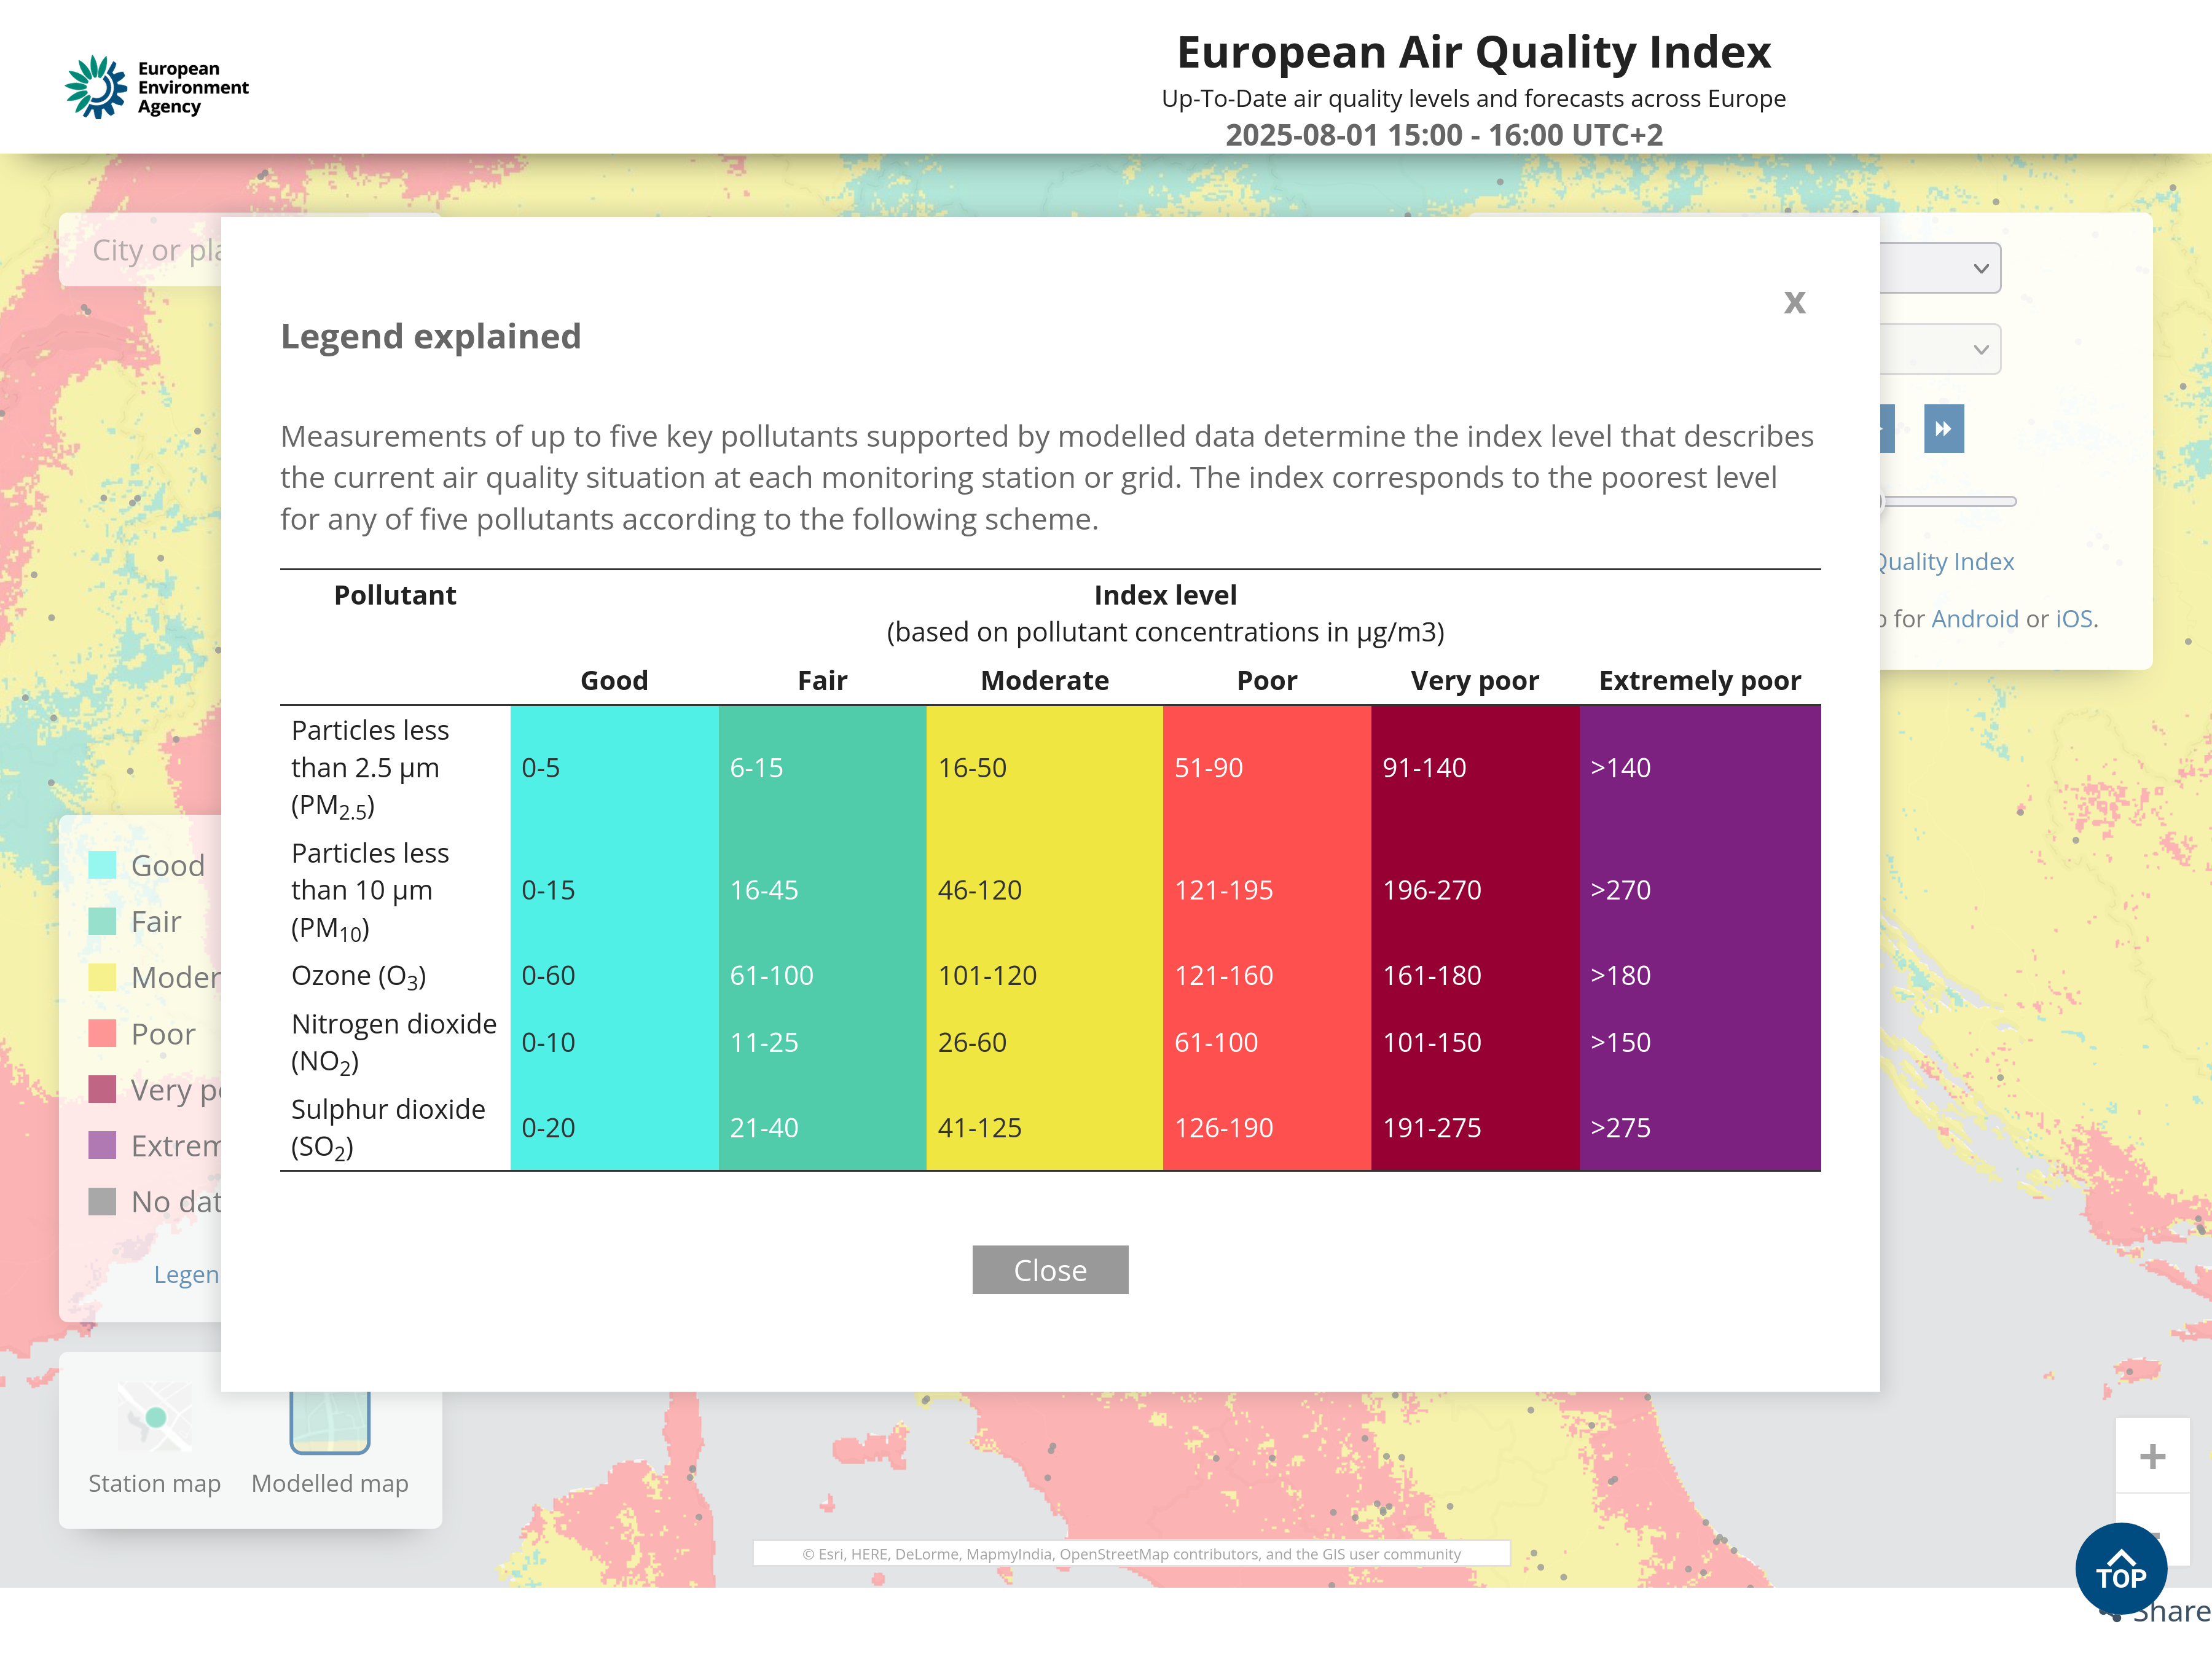
\includegraphics[width=\textwidth]{eea_4.png}
%   %\includegraphics[width=5cm]{figura.eps}%inserisce una figura larga 5cm
%   \caption[legenda elenco figure]{legenda sotto la figura}
%   \label{fig:prima}
% \end{figure}


\section{Principali inquinanti atmosferici e loro origini}

La valutazione della qualità dell'aria si basa sul monitoraggio di specifici contaminanti presenti nell'atmosfera.
Secondo \citet{GoogleMapsAirQuality2024}, i parametri più frequentemente rilevati nelle aree urbane includono:

\subsection{Materiale particolato (PM)}

Insieme di particelle microscopiche solide e liquide sospese nell'atmosfera.
Le frazioni PM$_{10}$ e PM$_{2,5}$ identificano particelle con diametro rispettivamente inferiore a 10 e 2,5 micrometri.
Le principali sorgenti comprendono:

\begin{itemize}
  \item Traffico veicolare e combustione nei motori
  \item Riscaldamento domestico a biomassa
  \item Processi industriali
  \item Fenomeni naturali come incendi boschivi e tempeste di sabbia
\end{itemize}

\subsection{Biossido di azoto NO2}

Gas caratteristico dell'inquinamento urbano, generato prevalentemente da:

\begin{itemize}
  \item Emissioni del trasporto su strada
  \item Attività industriali
  \item Impianti di produzione energetica
  \item Sistemi di riscaldamento civile
\end{itemize}

\subsection{Ozono troposferico O3}

Diversamente dall'ozono stratosferico che ci protegge dai raggi UV, quello presente negli strati bassi dell'atmosfera
costituisce un inquinante secondario. Si forma attraverso reazioni fotochimiche tra:

\begin{itemize}
  \item Composti organici volatili
  \item Ossidi di azoto
  \item Radiazione solare
\end{itemize}

Le fonti primarie dei precursori sono veicoli, centrali termoelettriche e processi industriali.

\subsection{Anidride solforosa SO2}

Gas dall'odore caratteristico e dalle proprietà irritanti, originato da:

\begin{itemize}
  \item Combustione di carbone e derivati petroliferi negli impianti energetici
  \item Raffinazione del petrolio
  \item Produzione di cemento
  \item Attività vulcanica
\end{itemize}

\subsection{Monossido di carbonio (CO)}

Gas inodore e tossico prodotto dalla combustione incompleta di combustibili fossili in veicoli e macchinari industriali.

\clearpage{\pagestyle{empty}\cleardoublepage}

\chapter{Tecnologie}
\label{chapter:second}

Nel seguente capitolo verranno presentate le tecnologie adottate per la realizzazione del progetto AirQualityInsight.
Data la natura di applicazione web del progetto, le tecnologie sono state classificate distinguendo tra quelle
utilizzate per il front-end e quelle per il back-end.

\section{Applicazioni front-end}

In questa sezione verranno presentate le principali tecnologie front-end impiegate nello sviluppo
del progetto AirQualityInsight.
L'applicazione front-end verrà sviluppata in Javascript utilizzando i seguenti framework:
\begin{itemize}
  \item Vue per lo sviluppo dell'architettura e della struttura generale dell'applicazione.
  \item Leaflet per la visualizzazione della mappa interattiva.
\end{itemize}

Di seguito, la descrizione dettagliata delle singole tecnologie.

\subsection{Vue}

Vue.js è un framework JavaScript progressivo per la costruzione di interfacce utente,
creato da Evan You nel 2014 \cite{vue2014}. Nato dall'esperienza dell'autore con AngularJS \cite{angularjs2010}
durante il suo periodo in Google, Vue è stato progettato per essere facilmente adottabile,
combinando le peculiarità di Angular e React \cite{react2013} con una curva di apprendimento più veloce
per gli sviluppatori che si interfacciano con esso.

La caratteristica distintiva di Vue risiede nella sua natura progressiva, che consente di adottarlo gradualmente in base
alle necessità del progetto. Al livello più elementare, Vue può essere utilizzato come una semplice libreria JavaScript
per arricchire pagine \acrshort{html} esistenti con funzionalità interattive. A livello intermedio invece, il framework
è in grado di gestire componenti complessi in relazione fra loro utilizzando sistemi di routing sofisticati. Infine,
al livello più avanzato, Vue permette la costruzione di \acrfull{spa} \cite{mdn2024spa} complete.

Il sistema di reattività costituisce uno dei pilastri fondamentali dell'architettura di Vue. Questo meccanismo
garantisce infatti la sincronizzazione automatica tra il modello dati e la vista, attraverso un sistema di
data binding bidirezionale, ossia un meccanismo di sincronizzazione automatica che mantiene allineati i dati tra
il modello dell'applicazione (model) e l'interfaccia utente (view) in entrambe le direzioni. Le computed properties
permettono la definizione di proprietà calcolate che si aggiornano automaticamente quando cambiano le loro dipendenze,
mentre i watchers offrono la possibilità di creare osservatori personalizzati per reagire a modifiche specifiche
dei dati.

Vue adotta un'architettura basata su componenti, in cui ciascun componente costituisce un elemento modulare e
riutilizzabile dell'interfaccia utente. I \acrfull{sfc}, caratterizzati dall'estensione \texttt{.vue},
incapsulano template \acrshort{html}, logica JavaScript e stili \acrshort{css} in un unico file,
facilitando la manutenzione e l'organizzazione del codice. La comunicazione tra componenti avviene attraverso
un sistema ben definito di props per il passaggio di dati da genitore a figlio e di eventi per la comunicazione inversa.

A livello tecnico, Vue implementa un sistema di template dichiarativo che utilizza una sintassi intuitiva. Il framework
utilizza un Virtual \acrshort{dom} per ottimizzare le prestazioni, effettuando confronti tra stati precedenti e nuovi
per minimizzare gli aggiornamenti del \acrshort{dom} reale.

L'ambiente Vue si caratterizza per la presenza di molteplici strumenti di tipologie differenti. Per la gestione e
compilazione dei progetti Vue, vengono maggiormente utilizzati Vue \acrshort{cli} \cite{vuecli2018} e
Vite \cite{vite2021}: Vue \acrshort{cli} permette la per la creazione e gestione di progetti da riga di comando,
mentre Vite rappresenta un build tool con tempi di compilazione ridotti e maggiore semplicità d'utilizzo.
Per il routing esiste Vue Router \cite{vuerouter2016}, il quale gestisce il routing nelle \acrfull{spa}.
Per la gestione centralizzata dello stato si hanno Vuex \cite{vuex2016} e Pinia \cite{pinia2021}.
Infine, per il debugging, Vue DevTools \cite{vuedevtools2016} fornisce strumenti avanzati attraverso estensioni
per browser.

L'evoluzione di Vue ha visto il passaggio da Vue 2, che ha consolidato l'adozione del framework nell'ambiente
enterprise, a Vue 3, rilasciato nel 2020. L'innovazione più significativa di questa major release è probabilmente la
Composition \acrshort{api}, che permette una migliore organizzazione della logica dei componenti e facilita la
riusabilità del codice rispetto alla Options \acrshort{api}. Inoltre, è stato migliorato il supporto nativo per il
Typescript e, con l'introduzione del supporto per il tree-shaking, sono state ridotte le dimensioni generali dei bundle.

In conclusione, Vue.js trova applicazione ideale nello sviluppo di applicazioni web moderne, dalle \acrfull{spa} alle
\acrfull{pwa}, dai dashboard amministrativi alle piattaforme e-commerce. La sua natura incrementale lo rende
particolarmente adatto per la migrazione graduale di applicazioni legacy e per la prototipazione rapida
di nuove funzionalità.

\subsection{Leaflet}

Leaflet rappresenta una delle librerie JavaScript open-source più popolari per la creazione di mappe interattive
ottimizzate per dispositivi mobili e l'integrazione di funzionalità cartografiche nelle applicazioni web.
Sviluppata inizialmente da Vladimir Agafonkin nel 2011 \cite{agafonkin2011leaflet} è stata successivamente mantenuta da
una comunità attiva di sviluppatori per la cartografia digitale.

I punti cardine di Leaflet sono la semplicità, l'efficienza e l'usabilità, qualità che lo rendono uno strumento di larga
diffusione per sviluppatori che necessitano di implementare mappe interattive senza la complessità di librerie più
pesanti, grazie anche ad un footprint di soli 39 KB di JavaScript compresso \cite{leafletnpm2024}.

L'architettura modulare di Leaflet costituisce uno dei suoi principali punti di forza. Tale libreria è stata infatti
progettata seguendo il principio della responsabilità singola (\acrshort{srp}), dove ogni componente gestisce
solo alcuni aspetti specifici della funzionalità cartografica. Questa approccio consente di scegliere di utilizzare
solo i moduli necessari per il proprio progetto, riducendo così l'impatto sulle prestazioni e
facilitando la manutenzione del codice.

Le funzionalità core di Leaflet includono la gestione di layer cartografici multipli, il supporto per vari formati di
tile server, la gestione di marker personalizzabili, popup informativi, controlli di navigazione e zoom interattivo.
La libreria supporta nativamente i più comuni sistemi di proiezione cartografica, con particolare attenzione alla
proiezione Web Mercator utilizzata dalla maggior parte dei servizi di tile moderni come \acrfull{osm} e Google Maps.

È possibile inoltre installare moduli accessori (plugin) sviluppati da terzi per integrare funzionalità aggiuntive.
Tali moduli vengono realizzati, mantenuti e resi disponibili dalla comunità open source. Questi vanno ad estendere le
funzionalità base della libreria, ad esempio, aggiungendo supporto per clustering di marker, drawing tools, integrazione
con servizi di geocoding, visualizzazione di heatmap, gestione di dati GPX e altro ancora. Questa modularità permette di
costruire applicazioni cartografiche complesse partendo da una base leggera e aggiungendo solo le funzionalità
effettivamente necessarie.

Dal punto di vista delle prestazioni, Leaflet implementa diverse ottimizzazioni per garantire un'esperienza
utente fluida. Il sistema di gestione dei tile implementa strategie di caching e lazy loading, caricando solo le
porzioni di mappa effettivamente presenti nell'area di visualizzazione. Il rendering dei marker è ottimizzato attraverso
tecniche di virtualizzazione che gestiscono efficientemente svariati punti disegnati sulla mappa senza appesantire
le prestazioni di scrolling e zoom.

L'\acrshort{api} di Leaflet offre un'interfaccia intuitiva e ben documentata che segue convenzioni JavaScript moderne.
La libreria supporta sia approcci programmatici tradizionali che pattern più moderni come la programmazione funzionale e
l'utilizzo di Promise per operazioni asincrone. L'integrazione con framework JavaScript contemporanei come Vue.js,
React e Angular è facilitata da wrapper specifici e da una architettura event-driven che si integra naturalmente con i
sistemi di reattività di questi framework.

La compatibilità cross-platform di Leaflet consente di supportare i browser moderni desktop e mobile.
La libreria gestisce automaticamente le differenze tra dispositivi touch e mouse, offrendo un'esperienza di navigazione
ottimizzata per ogni tipo di interfaccia.

Dal punto di vista della personalizzazione, Leaflet offre un controllo granulare sull'aspetto e il comportamento
delle mappe. Il sistema di styling basato su \acrshort{css} permette di personalizzare completamente l'aspetto
dei controlli, marker e popup, mentre l'\acrshort{api} JavaScript consente di definire
comportamenti  interattivi complessi.
La libreria supporta la creazione di marker personalizzati utilizzando \acrshort{html}, \acrshort{css} e \acrshort{svg},
permettendo la realizzazione di interfacce cartografiche su misura.

L'integrazione con servizi di tile esterni è una delle principali caratteristiche del framework, che consentono di
supportare nativamente servizi come OpenStreetMap, Google Maps, HERE ed altri.
Questa flessibilità permette agli sviluppatori di scegliere il provider di tile più adatto alle proprie esigenze
in termini di qualità, copertura geografica e costi, mantenendo la stessa \acrshort{api} di sviluppo.

La libreria dei dati geografici supporta il formato GeoJSON nativo, permettendo la visualizzazione di geometrie
complesse come poligoni, linee e punti direttamente da dati strutturati, come le aree comunali ed i confini
territoriali ed amministrativi di regioni, province ed altre suddivisioni geografiche.
L'integrazione con servizi \acrshort{rest} e \acrshort{api} geografiche è semplificata dalla gestione intrinseca di
richieste \acrshort{ajax} e dalla capacità di processare dati in tempo reale.

La community di Leaflet mantiene attivo il core della libreria e contribuisce con supporto tecnico, numerosi plugin,
tutorial, esempi d'utilizzo ed una documentazione ufficiale completa ed aggiornata.

In termini di performance e scalabilità, Leaflet gestisce elasticamente applicazioni di varia natura e dimensione.
Per le applicazioni più semplici, la libreria offre una soluzione plug-and-play che richiede configurazione minima
per installare le sole funzionalità necessarie, in modo da migliorare l'esperienza d'utilizzo.

Il seguente esempio \ref{lst:leaflet} mostra come sia possibile realizzare una mappa con tile \acrfull{osm}
centrata su Piazza Maggiore (Bologna), ottenendo la mappa mostrata in figura \ref{fig:leaflet}:

\begin{lstlisting}[caption={Mappa Bologna con Leaflet}, label=lst:leaflet]
  // Coordinates of Piazza Maggiore
  const lat = 44.4939;
  const lng = 11.3426;

  const map = L.map('map').setView([lat, lng], 13);

  // Tiles layer (OpenStreetMap)
  L.tileLayer('https://{s}.tile.openstreetmap.org/{z}/{x}/{y}.png', {
    maxZoom: 19,
    attribution: '<a href="http://www.openstreetmap.org/copyright">OpenStreetMap</a>'
  }).addTo(map);

  // Current position marker
  const marker = L.marker([lat, lng]).addTo(map);

  // Marker popup
  marker.bindPopup(`
    <div style="text-align: center;">
      <h4>Piazza Maggiore, Bologna</h4>
      <p>Lat: ${lat}</p>
      <p>Lng: ${lng}</p>
    </div>
  `).openPopup();

  // Circle on area
  L.circle([lat, lng], {
    color: 'red',
    fillColor: '#f03',
    fillOpacity: 0.2,
    radius: 1000 // meters
  }).addTo(map);

  // Optional controls
  L.control.scale({
    imperial: false,
    metric: true
  }).addTo(map);
\end{lstlisting}

\begin{figure}[H]
  \centering
  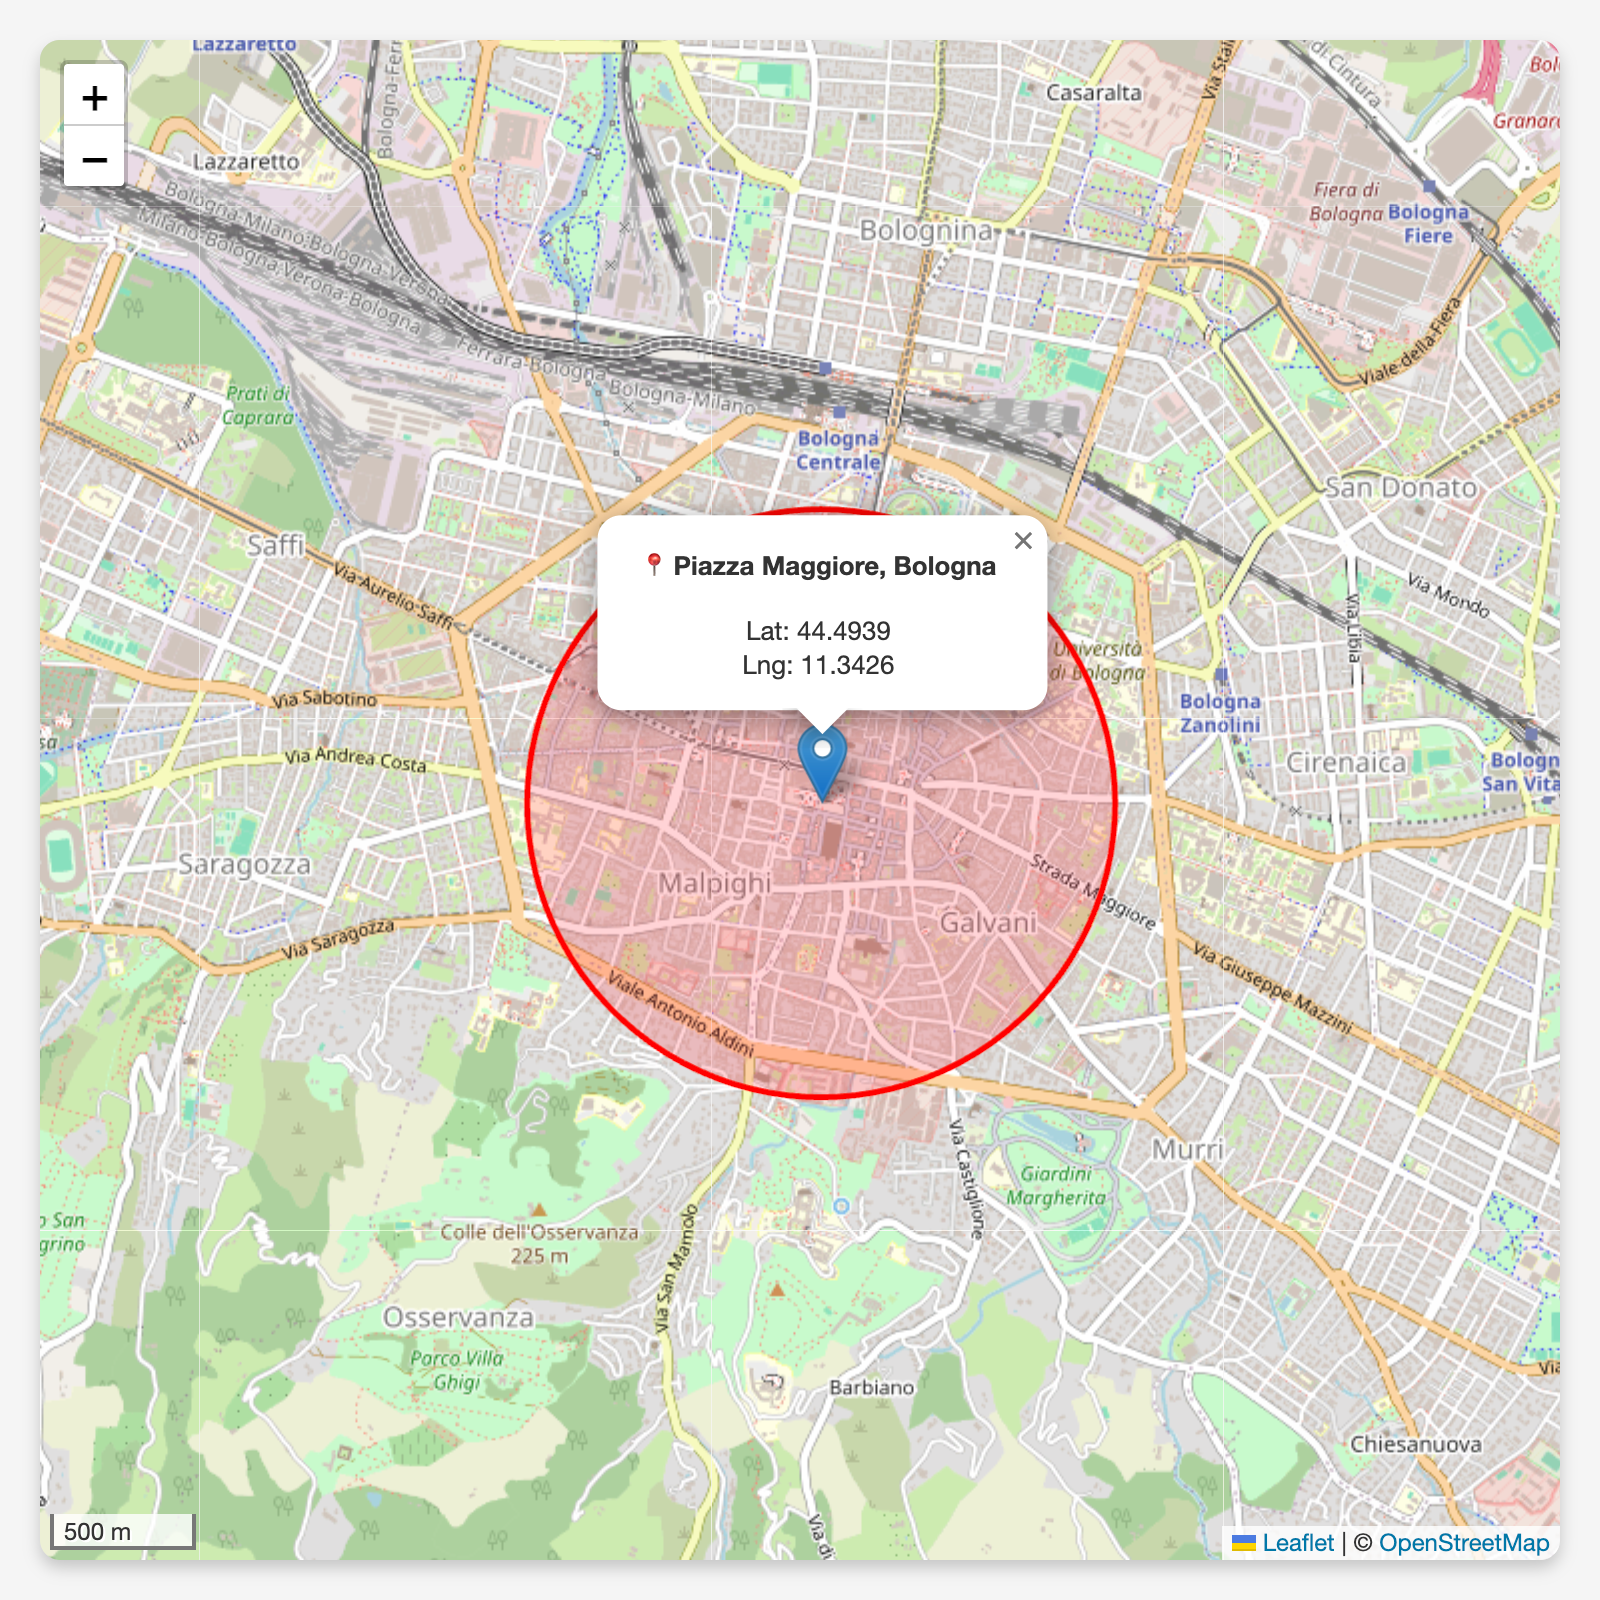
\includegraphics[width=\textwidth]{leaflet.png}
  \caption{Piazza Maggiore, Bologna}
  \label{fig:leaflet}
\end{figure}

In conclusione, Leaflet si posiziona come una soluzione affidabile per l'integrazione di funzionalità cartografiche
in applicazioni web moderne. Combinando leggerezza, potenza, estensibilità e facilità d'uso diventa una scelta indicata
per sviluppatori che necessitano di implementare mappe interattive performanti e personalizzabili, dal prototipo rapido
all'applicazione complessa.

\section{Applicazioni back-end}

In questa sezione verranno presentate le principali tecnologie back-end impiegate nello sviluppo del progetto
AirQualityInsight.

Verranno utilizzati Node.js per realizzare il server, Python per simulare i dispositivi di misurazione della
qualità dell'aria, Kafka come broker dei messaggi e MongoDB per mantenere un database documentale delle registrazioni.

\subsection{Node.js}

Node.js è un runtime system open-source multipiattaforma costruito sul motore JavaScript V8
di Google Chrome \citep{capan_2013_nodejs}. A differenza dei tradizionali ambienti JavaScript che operano esclusivamente
nel browser, Node.js permette l'esecuzione di codice JavaScript lato server, abilitando lo sviluppo di applicazioni web
complete utilizzando un unico linguaggio di programmazione.

Le principali caratteristiche di Node.js sono l'adozione di un paradigma event-driven,
un approccio non-blocking I/O ed un processo single-threaded. Il modello di programmazione orientato agli eventi
consente di gestire efficientemente operazioni asincrone basate sulla manifestazione di determinati eventi.
Le operazioni di input e di output non bloccanti migliorano le performance dell'applicativo.
L'uso di un singolo thread principale con un event loop riduce la complessità della gestione della concorrenza.

Il seguente esempio \ref{lst:node-server} mostra come creare un server \acrshort{http} minimale utilizzando Node.js:

\begin{lstlisting}[caption={Server \acrshort{http} base in Node.js}, label=lst:node-server]
const http = require('http');

const server = http.createServer((req, res) => {
  res.writeHead(200, {'Content-Type': 'text/plain'});
  res.end('Hello world!');
});

const PORT = 3000;
server.listen(PORT, () => {
  console.log(`Server listening on port ${PORT}`);
});
\end{lstlisting}

Node.js offre ampie funzionalità per l'interazione con il file system.
L'esempio seguente \ref{lst:node-fs} dimostra la lettura asincrona di un file:

\begin{lstlisting}[caption={Lettura asincrona di file}, label=lst:node-fs]
const fs = require('fs');

// Asynchronous reading
fs.readFile('file.txt', 'utf8', (err, data) => {
  if (err) {
    console.error('Error in file reading:', err);
    return;
  }
  console.log('File content:', data);
});

// Synchronous reading (not file for large files)
try {
  const data = fs.readFileSync('example.txt', 'utf8');
  console.log('File content:', data);
} catch (err) {
  console.error('Error in file reading:', err);
}
\end{lstlisting}

L'architettura di Node.js si basa sul concetto di event loop, un meccanismo che permette di gestire multiple operazioni
I/O senza bloccare l'esecuzione del programma principale \citep{nodejs_docs_2023}. Questo approccio lo rende
particolarmente adatto per applicazioni che richiedono alta concorrenza con operazioni I/O intensive,
come \acrshort{api} \acrshort{rest}, applicazioni real-time su dispositivi distribuiti e microservizi.

Le performance di Node.js sono generalmente migliori rispetto ai server tradizionali multi-threaded per applicazioni
I/O-bound, grazie alla riduzione dell'overhead dovuto al context switching tra thread e alla gestione efficiente della
memoria. Questo poiché i sistemi tradizionali adottano tecniche di gestione delle richieste creando un nuovo thread
per ogni nuova connessione, mentre Node.js, operando su un singolo thread ed utilizzando chiamate I/O non bloccati,
riesce a supportare un maggior numero di richieste concorrenti nell'event loop.

Quello che ha reso popolare tale framework è la praticità e la versatilità che lo contraddistinguono.
Risulta infatti una buona scelta nel realizzare velocemente applicazioni web scalabili, grazie alla sua capacità
di gestire un numero elevato di connessioni simultanee.

Node.js dispone di un gestore di pacchetti chiamato ``\acrshort{npm}'' (\acrlong{npm}), il quale fornisce un insieme
di librerie e componenti riutilizzabili e disponibili al pubblico, facilmente installabili tramite un repository online,
con gestione delle versioni e delle dipendenze. Tali librerie sono accessibili attraverso uno strumento
command-line dedicato.

I moduli principali sono:
\begin{itemize}
  \item Express, un framework di sviluppo web \cite{express_js};
  \item Socket.io, un componente server-side di due WebSocket components comuni \cite{socket_io};
  \item Mongodb, che fornisce \acrshort{api} per l'omonimo database \cite{mongodb};
  \item Redis, un sistema di caching \cite{redis}.
\end{itemize}
È possibile per chiunque realizzare e pubblicare la propria libreria su \acrfull{npm}.

In conclusione, Node.js rappresenta una soluzione moderna e efficace per lo sviluppo di applicazioni server-side,
disponendo di una vasta scelta di librerie disponibili attraverso \acrfull{npm} ed una community attiva.
La sua architettura event-driven e le performance elevate lo rendono una scelta ideale per molte tipologie
di applicazioni web moderne.

\subsubsection{\acrshort{wot}}

Il Web of Things (\acrshort{wot}) rappresenta un paradigma architetturale che estende i principi del \acrshort{www}
all'\acrshort{iot}, permettendo l'interoperabilità tra dispositivi eterogenei attraverso standard
web consolidati~\cite{w3c-wot-td}. L'implementazione analizzata trasforma sensori di qualità dell'aria in
\textit{Things} web-accessibili, seguendo le specifiche \acrshort{w3c} e utilizzando l'ontologia
\acrfull{saref}~\cite{saref-ontology}. Ogni sensore fisico viene quindi trasformato in una risorsa web
identificabile univocamente, accessibile attraverso protocolli \acrshort{http} standard e descritta mediante metadati
strutturati secondo il vocabolario \acrshort{wot}. Questa approccio garantisce l'interoperabilità semantica e
l'integrazione seamless con applicazioni web esistenti.

L'architettura utilizza le \acrfull{td} come elemento centrale, conformi alla specifica \acrshort{w3c} \acrshort{wot}
\acrlong{td} v1.1~\cite{w3c-wot-td}. La struttura della \acrshort{td} include diversi componenti fondamentali
che definiscono l'identità, le capacità e le modalità di interazione del dispositivo. Ogni sensore viene identificato
univocamente attraverso \acrshort{uri} strutturati (urn:sensor:air-quality:\$\{sensor\_id\}) e classificato
semanticamente usando il tipo saref:Sensor.

Il contesto semantico integra il vocabolario \acrshort{wot} standard con l'ontologia \acrshort{saref},
facilitando l'interpretazione automatica delle funzionalità del dispositivo. Le proprietà modellano
parametri ambientali con schemi di dati precisi che includono tipo, unità di misura e range di validità.

La directory \acrshort{wot} (\texttt{/wot/things}) supporta il discovery automatico dei dispositivi,
fornendo informazioni sommarie su identità, stato operativo e ultimo contatto.
Le notifiche proattive via WebSocket mantengono sincronizzate le applicazioni client senza polling periodico.

L'implementazione rispetta le specifiche \acrshort{w3c} \acrshort{wot}~\cite{w3c-wot-architecture}, utilizzando
vocabolari semantici standard e implementando gli elementi necessari.
L'uso dell'ontologia \acrshort{saref}~\cite{saref-ontology} aggiunge un layer semantico che facilita
l'interoperabilità con sistemi di building automation e smart city.

La separazione tra modello logico (\acrlong{td}) e implementazione fisica (sensori hardware) facilita l'evoluzione
dell'architettura e l'integrazione di nuove tipologie di dispositivi, confermando la validità del paradigma
\acrshort{wot} per applicazioni \acrshort{iot} di larga scala e garantiscono compatibilità
con toolchain \acrshort{wot} esistenti e scalabilità orizzontale~\cite{guinard-wot}.

\subsection{Python}

Python è un linguaggio di programmazione di alto livello, interpretato e multi-paradigma.
È stato creato da Guido Van Rossum e rilasciato per la prima volta nel 1991 \citep{van_rossum_1995}.
Il nome deriva dalla serie televisiva britannica "Monty Python's Flying Circus", riflettendo l'approccio creativo
che caratterizza l'intera filosofia del linguaggio.

La filosofia di Python è codificata nel famoso "Zen of Python" di Tim Peters, un insieme di principi guida
che enfatizzano la leggibilità, la semplicità e la qualità del codice. Tra questi principi spicca il motto
\textit{"Beautiful is better than ugly"} e \textit{"Simple is better than complex"}, che hanno influenzato profondamente
la progettazione del linguaggio e la sua evoluzione nel corso degli anni \citep{peters_2004}.

Uno degli elementi che contraddistinguono Python rispetto ad altri linguaggi di programmazione è l'assenza di parentesi
graffe per delimitare i blocchi di codice, ma bensì l'utilizzo dell'indentazione stessa. Tale caratteristica ha promosso
l'apprendimento del linguaggio a programmatori alle prime armi, che hanno potuto così concentrarsi maggiormente sul
contenuto del codice grazie alla sua forma più pulita e leggibile.

Il supporto di diversi modelli di programmazione da parte di Python lo ha reso un linguaggio versatile e popolare.
Si possono infatti scegliere approcci procedurali per script semplici, orientati agli oggetti per applicazioni più
complesse o funzionali per elaborazioni matematiche più avanzate. Questa flessibilità permette di scegliere il paradigma
migliore per il problema specifico da risolvere.

Una peculiarità del linguaggio Python è il concetto dove tutto è un oggetto, inclusi numeri, stringhe,
funzioni e persino le classi stesse. Tale uniformità concettuale semplifica notevolmente il modello mentale necessario
per comprendere il linguaggio, facilitando quindi l'apprendimento di concetti avanzati.

Il sistema di tipizzazione è forte (strong typing) ed eseguito a run-time (dynamic typing), evitando così errori comuni
dipesi dalle operazioni implicite tra tipi incompatibili. È stato introdotto il supporto per type hints, permettendo
di annotare esplicitamente i tipi delle variabili e dei parametri delle funzioni. Queste annotazioni, pur non
influenzando l'esecuzione del programma, migliorano significativamente la leggibilità del codice e abilitano strumenti
di analisi statica per la rilevazione precoce di errori di tipo.

Python gestisce in autonomia la memoria allocata grazie ad un sistema garbage collector.
Questo solleva il programmatore dalla necessità di gestire manualmente l'allocazione e la deallocazione della memoria,
riducendo drasticamente i bug legati alla gestione delle risorse. Il garbage collector rappresenta un utile strumento
che, sfruttando il reference counting ed integrato con un rilevatore di cicli, permette di individuare e segnalare
riferimenti circolari.

Anche se spesso viene inteso come linguaggio interpretato, Python in realtà non converte direttamente
il codice sorgente in linguaggio macchina, ma passa prima una fase di pre-compilazione bytecode, evitando di
reinterpretare integralmente il codice e migliorando le prestazioni.

L'ecosistema di Python è arricchito dal \acrfull{pypi}, un repository centrale che ospita centinaia di migliaia di
pacchetti di terze parti \citep{pypi_2023}. Viene così  praticamente ricoperto ogni dominio applicativo,
dalla sviluppo web all'intelligenza artificiale, dall'analisi dei dati alla computer vision.

Il sistema di gestione dei pacchetti, principalmente attraverso pip, rende estremamente semplice l'installazione e la
gestione delle dipendenze. L'introduzione di strumenti come virtualenv e, più recentemente, pipenv e poetry,
ha ulteriormente migliorato la gestione degli ambienti di sviluppo isolati, permettendo di evitare conflitti
tra diverse versioni delle librerie. Questo risulta molto comodo qualora si lavori a progetti che utilizzando versioni
differenti delle dipendenze.

La libreria standard provvede un ricco numero di moduli base, come quelli per le operazioni su file system, networking,
regex, database, threading, e molto altro. Questa completezza riduce la necessità di dipendenze esterne per molte
operazioni comuni.

Uno dei campi in cui il linguaggio è maggiormente usato è quello scientifico, dove librerie come NumPy e SciPy
hanno trasformato Python in uno strumento fondamentale per il calcolo numerico,
fornendo strutture dati efficienti e algoritmi ottimizzati per operazioni matematiche complesse.
Pandas ha rivoluzionato l'analisi dei dati, offrendo strutture dati potenti per la manipolazione e l'analisi
di dataset strutturati.

Il seguente esempio \ref{lst:measurements} mostra come sia possibile generare misurazioni aleatorie in Python:

\begin{lstlisting}[caption={Generazione di misurazioni aleatorie in Python}, label=lst:measurements]
import random
import numpy as np
from datetime import datetime, timedelta

class MeasurementGenerator:
  def __init__(self):
    self.sensors = {
      'temperature': {'min': 15, 'max': 35, 'unit': 'C'},
      'humidity': {'min': 30, 'max': 90, 'unit': '%'},
      'pressure': {'min': 990, 'max': 1030, 'unit': 'hPa'}
    }

  def generate_measurement(self, sensor_type):
      config = self.sensors[sensor_type]
      value = random.uniform(config['min'], config['max'])
      return {
        'timestamp': datetime.now().isoformat(),
        'sensor': sensor_type,
        'value': round(value, 2),
        'unit': config['unit']
      }

  def generate_time_series(self, sensor_type, hours=24, interval_minutes=60):
    measurements = []
    start_time = datetime.now() - timedelta(hours=hours)

    for i in range(0, hours * 60, interval_minutes):
      timestamp = start_time + timedelta(minutes=i)
      config = self.sensors[sensor_type]

      base_value = (config['min'] + config['max']) / 2
      daily_variation = 5 * np.sin(2 * np.pi * i / (24 * 60))
      noise = random.gauss(0, 1)
      value = base_value + daily_variation + noise

      measurements.append({
        'timestamp': timestamp.isoformat(),
        'sensor': sensor_type,
        'value': round(np.clip(value, config['min'], config['max']), 2),
        'unit': config['unit']
      })

    return measurements

if __name__ == '__main__':
  generator = MeasurementGenerator()

  single_measurement = generator.generate_measurement('temperature')
  print(f"Single: {single_measurement}")

  time_series = generator.generate_time_series('temperature', hours=12)
  print(f"Generated {len(time_series)} measurements")
  print(f"First: {time_series[0]}")
  print(f"Last: {time_series[-1]}")
\end{lstlisting}

Eseguendo il codice riportato nell'esempio \ref{lst:measurements} si può ottenere un output come riportato
in lista \ref{lst:measurements-output}:
\begin{lstlisting}[caption={Output di esempio ottenuto dalla generazione di misurazioni aleatorie in Python},
  label=lst:measurements-output]
  Single: {'timestamp': '2025-08-28T18:55:41.327822', 'sensor': 'temperature', 'value': 30.71, 'unit': 'C'}
  Generated 12 measurements
  First: {'timestamp': '2025-08-28T05:55:41.327850', 'sensor': 'temperature', 'value': 25.79, 'unit': 'C'}
  Last: {'timestamp': '2025-08-28T22:55:41.327850', 'sensor': 'temperature', 'value': 26.01, 'unit': 'C'}
\end{lstlisting}

Anche nello sviluppo web, Python rimane una delle scelte preferire dagli sviluppatori, i quali possono usare framework
come Django e Flask \citep{django_2023, flask_2023} per realizzare le proprie applicazioni web.
Fra i due, Flask risulta più minimale e flessibile per progetti che richiedono un controllo più granulare
dell'architettura, mentre Django include tutto il necessario per sviluppare sistemi complessi.

Il seguente esempio \ref{lst:flask} mostra come sia possibile realizzare un semplice server usando Flask:

\begin{lstlisting}[caption={Server Flask base in Python}, label=lst:flask]
from flask import Flask, jsonify, request

app = Flask(__name__)

users = [
  {"id": 1, "name": "John", "email": "john@example.com"},
  {"id": 2, "name": "Jane", "email": "jane@example.com"}
]

@app.route('/')
def home():
  return {"message": "Flask server running", "users_count": len(users)}

@app.route('/api/users', methods=['GET'])
def get_users():
  return jsonify(users)

@app.route('/api/users/<int:user_id>', methods=['GET'])
def get_user(user_id):
  user = next((u for u in users if u["id"] == user_id), None)
  if user:
    return jsonify(user)
  return jsonify({"error": "User not found"}), 404

@app.route('/api/users', methods=['POST'])
def create_user():
  data = request.get_json()
  if not data or 'name' not in data or 'email' not in data:
    return jsonify({"error": "Name and email required"}), 400

  new_user = {
    "id": max([u["id"] for u in users]) + 1,
    "name": data["name"],
    "email": data["email"]
  }
  users.append(new_user)
  return jsonify(new_user), 201

if __name__ == '__main__':
  app.run(debug=True, port=5000)
\end{lstlisting}

Eseguendo il codice riportato nell'esempio \ref{lst:flask} si può ottenere un output come riportato
in lista \ref{lst:flask-output}:
\begin{lstlisting}[caption={Output di esempio ottenuto dall'interazione con le rotte disposte dal server web in Flask},
  label=lst:flask-output]
  // Main url
  curl 127.0.0.1:5000
  {
    "message": "Flask server running",
    "users_count": 2
  }

  // Get all users
  curl 127.0.0.1:5000/api/users
  [
    {
      "email": "john@example.com",
      "id": 1,
      "name": "John"
    },
    {
      "email": "jane@example.com",
      "id": 2,
      "name": "Jane"
    }
  ]

  // Show informations about user #1
  curl 127.0.0.1:5000/api/users/1
  {
    "email": "john@example.com",
    "id": 1,
    "name": "John"
  }

  // Show informations about user #2
  curl 127.0.0.1:5000/api/users/2
  {
    "email": "jane@example.com",
    "id": 2,
    "name": "Jane"
  }

  // Create new user
  curl -X POST http://127.0.0.1:5000/api/users \
    -H "Content-Type: application/json" \
    -d '{"name": "Mario Rossi", "email": "mario.rossi@example.com"}'
  {
    "email": "mario.rossi@example.com",
    "id": 3,
    "name": "Mario Rossi"
  }
\end{lstlisting}


L'approccio "pythonic" enfatizza la leggibilità del codice e la rapidità di sviluppo, permettendo di creare prototipi
funzionali in tempi molto brevi e di scalare gradualmente verso applicazioni enterprise.

Sempre nel campo scientifico, Python è diventato il linguaggio de-facto per data science e machine learning,
grazie alle librerie specializzate. TensorFlow e PyTorch, ad esempio, hanno reso accessibili le tecniche di
deep learning senza il bisogno di avere nozioni approfondite di matematica avanzata.

Un altro campo in cui il linguaggio è fortemente utilizzato è quello delle DevOps e dell'amministrazione di sistemi,
grazie alla capacità di interagire facilmente con il sistema operativo, nel processare file di testo, interfacciarsi
con database e \acrshort{api} \acrshort{rest}. Viene infatti scelto per automatizzare processi ripetitivi,
creare pipeline di elaborazione dati ed integrazione di sistemi eterogenei, settori dove la rapidità di sviluppo e la
manutenibilità del codice sono cruciali.

Python rimane uno dei linguaggi più popolari e trasversali, godendo di una forte comunità che ne segue gli sviluppi e lo
aggiorna in modo continuativo, con rilasci annuali che introducono nuove funzionalità e miglioramenti delle performance.
L'adozione crescente in settori come l'intelligenza artificiale, l'\acrfull{iot} e l'edge computing suggerisce che
Python rimarrà rilevante e in continua evoluzione, adattandosi alle esigenze di un panorama tecnologico
in rapido cambiamento.

\subsection{Kafka}

Apache Kafka è una piattaforma di streaming distribuito basato su Java e Scala, progettata per gestire flussi di dati
in tempo reale su larga scala \cite{narkhede2017kafka}. Sviluppato originariamente da LinkedIn e successivamente
donato alla Apache Software Foundation nel 2011, Kafka ha acquisito presto popolarità nel panorama
della messaggistica e del processing di eventi in sistemi distribuiti \cite{garg2013apache}.

La filosofia di Kafka si basa sul concetto di event streaming, dove i dati vengono trattati come una sequenza immutabile
di eventi che possono essere pubblicati, memorizzati e processati in tempo reale \cite{stopford2018designing}.
Questo paradigma si discosta significativamente dai tradizionali message broker, offrendo persistenza duratura,
elevata throughput e capacità di replay dei messaggi, caratteristiche fondamentali per architetture moderne
basate su microservizi e event-driven architecture.

L'architettura distribuita di Kafka consente la gestione in tempo reale di grandi volumi di dati,
rendendolo una valida scelta in campi quali analytics, monitoring, fraud detection e real-time recommendation systems
\cite{kreps2014kafka}. Il sistema organizza i dati in topic, entità logiche che rappresentano categorie di messaggi
correlati \cite{narkhede2017kafka}. Ogni topic è suddiviso in partition, unità fisiche di parallelizzazione
che permettono la distribuzione del carico e la scalabilità orizzontale del sistema.

Il modello di persistenza di Kafka utilizza un commit log distribuito, dove ogni messaggio viene assegnato a un offset
sequenziale all'interno di una partizione \cite{garg2013apache}. Questa struttura garantisce l'ordinamento dei messaggi
all'interno di ciascuna partizione e permette un accesso efficiente, sia sequenziale che random, ai dati storici.
La persistenza è implementata attraverso segment files ottimizzati per operazioni append-only, minimizzando la latenza
di scrittura e massimizzando la throughput.

I broker Kafka formano un cluster distribuito che gestisce la replica dei dati attraverso il meccanismo di
leader-follower replication \cite{stopford2018designing}. Ogni partizione ha un broker leader che gestisce tutte le
operazioni di lettura e scrittura, mentre i follower mantengono copie sincronizzate dei dati. Il sistema di elezione
del leader, basato su Apache ZooKeeper (e successivamente su KRaft metadata management),
garantisce alta disponibilità e fault tolerance.

Il modello publish-subscribe di Kafka si basa sull'interazione tra produttori, che pubblicano messaggi sui
topic, e consumatori, che leggono e processano questi messaggi \cite{kreps2014kafka}.
I produttori possono configurare diverse strategie di partitioning, utilizzando chiavi di partizionamento per garantire
che messaggi correlati vengano sempre inviati alla stessa partizione, preservando l'ordinamento temporale.

Kafka supporta diverse semantiche di delivery \cite{narkhede2017kafka}: la semantica at-least-once garantisce che
ogni messaggio venga consegnato almeno una volta, ma può comportare duplicazioni; la semantica at-most-once assicura
l'assenza di duplicati ma può causare perdite di messaggi in caso di failure; la semantica exactly-once,
introdotta nelle versioni più recenti, combina transazioni e idempotenza per garantire elaborazione esatta dei messaggi.

I consumer groups rappresentano un meccanismo di parallelizzazione del consumo di messaggi \cite{garg2013apache}.
Ogni consumer all'interno di un gruppo riceve messaggi da un sottoinsieme delle partizioni del topic,
permettendo scalabilità orizzontale del processing. Il consumer group rebalancing automatico redistribuisce
le partizioni tra i consumatori attivi, favorendo load balancing dinamico e fault tolerance.

Kafka Streams costituisce una libreria client per il processing di stream di dati che elimina la necessità di framework
esterni per elaborazioni in tempo reale \cite{stopford2018designing}. Questa libreria implementa il paradigma di stream
processing attraverso topology di trasformazioni che possono includere operazioni di filtering, mapping,
aggregation e joining tra stream differenti.

La scalabilità orizzontale di Kafka è limitata principalmente dal numero di partizioni per topic, che determina il
massimo grado di parallelismo achievable \cite{narkhede2017kafka}. L'aggiunta di broker al cluster permette
di aumentare la capacità di storage e processing, ma richiede careful planning del numero di partizioni e della
strategia di replica. Il processo di partition reassignment può essere utilizzato per bilanciare il carico
tra broker esistenti e nuovi.

Kafka si rivela particolarmente efficace in architetture event-driven dove la decoupling tra componenti e la capacità
di replay degli eventi sono requisiti fondamentali \cite{stopford2018designing}.
Pattern architetturali come Event Sourcing, \acrfull{cqrs} e Saga pattern sono indicati per tale strumento.

I casi d'uso tipici di Kafka includono real-time analytics, log aggregation, metrics collection, stream processing
per machine learning e data pipeline per data lake e data warehouse \cite{kreps2014kafka}.
La capacità di Kafka di fungere sia da message broker che da storage system può essere sfruttata in architetture
dove i dati devono essere processati da multiple applicazioni con diverse temporal requirements.

\subsection{MongoDB}

MongoDB è uno dei database NoSQL orientati ai documenti più noti ed utilizzati \cite{chodorow2013mongodb}.
Sviluppato inizialmente da 10gen (ora MongoDB Inc.) nel 2009, questo database ha rivoluzionato il modo in cui
gli sviluppatori approcciano la persistenza dei dati, offrendo un'alternativa flessibile e scalabile
ai tradizionali database relazionali \cite{banker2011mongodb}.

La filosofia alla base di MongoDB si discosta significativamente dal paradigma relazionale in favore di un modello
basato su documenti \acrfull{bson} che permette una maggiore flessibilità nella strutturazione
dei dati \cite{plugge2010mongodb}. Questa caratteristica consente agli sviluppatori di memorizzare
oggetti complessi e annidati senza la necessità di normalizzazione, tipica dei database SQL tradizionali.

L'architettura di MongoDB si avvale di un approccio document-oriented, dove ogni record è rappresentato come
un documento flessibile che può contenere campi di diversi tipi di dati \cite{harrison2015mongodb}.
Questa struttura elimina la rigidità dello schema fisso, permettendo l'evoluzione dinamica delle strutture dati
durante il ciclo di vita dell'applicazione.

Il sistema di indicizzazione di MongoDB supporta indici di varia natura quali composti, testuali, geospaziali ed altro,
offrendo prestazioni ottimizzate per diversi tipi di query \cite{membrey2014definitive}.
Gli indici vengono implementati utilizzando strutture dati B-tree per ottenere operazioni di ricerca efficienti
anche su grandi volumi di dati. Inoltre, MongoDB supporta indici parziali e \acrfull{ttl}, consentendo una gestione
automatica dei dati basata su criteri temporali.

La gestione della memoria in MongoDB utilizza il memory mapping per migliorare le prestazioni di lettura e scrittura
\cite{dayley2014mongodb}. Il WiredTiger storage engine ottiene ciò attraverso la compressione dei dati e il controllo
della concorrenza a livello di documento.

MongoDB utilizza un linguaggio di query basato su JavaScript che si integra naturalmente con gli ambienti
di sviluppo web moderni \cite{harrison2015mongodb}. Le query vengono espresse attraverso documenti \acrshort{json}
che specificano i criteri di ricerca, proiezione e ordinamento. Questa sintassi risulta particolarmente intuitiva
per gli sviluppatori familiari con JavaScript e altri linguaggi di programmazione moderni.

L'Aggregation Framework rappresenta uno strumento potente per l'elaborazione e l'analisi dei dati,
offrendo funzionalità comparabili a quelle dei sistemi SQL attraverso pipeline di trasformazione
\cite{membrey2014definitive}. Le operazioni di aggregazione includono filtering, grouping, sorting,
reshaping e computational operations, permettendo analisi complesse direttamente a livello di database.

Le prestazioni di MongoDB dipendono significativamente dalla progettazione dello schema e dalla strategia
di indicizzazione adottata \cite{chodorow2013mongodb}. A differenza dei database relazionali,
dove la normalizzazione è spesso prioritaria, in MongoDB è frequentemente vantaggioso denormalizzare i dati
per ottimizzare le performance di lettura.

MongoDB si rivela particolarmente efficace in scenari caratterizzati da rapido sviluppo,
schema evolutivo e necessità di scalabilità orizzontale \cite{banker2011mongodb}.
Applicazioni web, sistemi di gestione contenuti, piattaforme di social media e applicazioni \acrshort{iot}
rappresentano casi d'uso ideali per questo database. Tuttavia, per applicazioni che richiedono
transazioni \acrshort{acid} complesse o relazioni complesse tra entità, i database relazionali
tradizionali possono risultare più appropriati.

Il seguente esempio \ref{lst:mongodb} presenta quale query di esempio in un database Mongodb:

\begin{lstlisting}[caption={Query MongoDB}, label=lst:mongodb]
  // Document example
  {
    "_id": ObjectId("..."),
    "station": "Bologna Piazza Maggiore",
    "coordinates": {"lat": 44.4939, "lng": 11.3426},
    "pm25": 35.2,
    "pm10": 42.8,
    "no2": 48.5,
    "o3": 62.1,
    "temperature": 22.5,
    "humidity": 65,
    "aqi": 78,
    "level": "Moderate",
    "timestamp": ISODate("2025-08-23T14:30:00Z")
  }

  // Find stations with PM2.5 above 25 micrograms per cube meter
  db.air_quality.find({"pm25": {$gt: 25}})

  // Find stations with good air quality level in previous 24 hours
  db.air_quality.find({
    "level": "Good",
    "timestamp": {$gte: new Date(Date.now() - 24*60*60*1000)}
  })

  // Daily average of PM2.5 per station
  db.air_quality.aggregate([
    {$match: {"timestamp": {$gte: ISODate("2025-08-23T00:00:00Z")}}},
    {$group: {_id: "$station", avg_pm25: {$avg: "$pm25"}, measurements: {$sum: 1}}},
    {$sort: {avg_pm25: -1}}
  ])
\end{lstlisting}

\section{Deployment}

In questa sezione verranno descritti gli strumenti adoperati nel deployment, quali Docker
come ambiente di containerizzazione e Docker compose come strumento d'orchestrazione dei container realizzati dal primo.

\subsection{Docker}

Docker è un progetto open-source, il cui sviluppo è a cura della Docker Inc, divenuto uno dei principali attori
nel campo dello sviluppo e deployment di applicazioni basate su container Linux \cite{mouat2015docker}.
Questa tecnologia di containerizzazione permette di incapsulare un'applicazione insieme a tutte le sue dipendenze
in un contenitore leggero e portabile, garantendo che l'applicazione funzioni in modo consistente fra differenti
sistemi operativi. Questo container rappresenta infatti un sistema isolato dove l'applicazione dispone di tutte
le librerie necessarie alla sua esecuzione.

La filosofia alla base di Docker è fondata sul concetto di "write once, run anywhere", permettendo agli sviluppatori
di creare applicazioni che possono essere eseguite senza modifiche sui sistemi operativi che supportano
Docker \cite{merkel2014docker}. I container Docker condividono il kernel del sistema operativo host, rendendoli
più efficienti rispetto alle tradizionali macchine virtuali in termini di utilizzo delle risorse e tempi di avvio.
Non è quindi necessario avere installati sul proprio sistema operativo strumenti usati dall'applicazione poiché
saranno disponibili direttamente all'interno del container.

I container Docker vengono costruiti sulla base di file Dockerfile, i quali riportano tutte le istruzioni necessarie
a realizzare l'immagine. Un'immagine Docker è un pacchetto completo e immutabile che contiene l'essenziale
per eseguire un'applicazione: codice, librerie, dipendenze, configurazioni. Funziona come uno "stampo digitale"
che garantisce la riproducibilità dell'ambiente software, eliminando i problemi di compatibilità tra diversi sistemi.

Le immagini sono costruite a livelli sovrapposti, dove ogni strato aggiunge componenti specifici, rendendo efficiente
sia l'archiviazione che la condivisione. Questo risulta ottimale quando immagini differenti necessitano di elementi
in comune, condividendo fra loro livelli e riducendo lo spazio utilizzato, gli eventuali tempi
di download e di compilazione degli stessi. Una volta creata, l'immagine rimane invariata e può essere utilizzata
per generare molteplici container identici, che rappresentano le istanze in esecuzione dell'applicazione.

Docker permette anche la realizzazione di volumi, per disporre di dati persistenti, e di reti, per mettere
in comunicazione più container fra loro. I volumi trovano impiego qualora sia necessario mantenere dati
una volta arrestata l'esecuzione di un container, come per i database. Le reti sono usate invece per sistemi
più complessi in cui due o più container devono poter comunicare. Un container può essere disposto su una o più reti
virtuali per interagire con altri container. Avere più reti può risultare utile nel caso in cui determinati container
abbiano bisogno di vedere solo altri container su certi livelli, distinguendo ad esempio
servizi di back-end e di front-end.

Nel seguente esempio viene mostrato come sia possibile realizzare un container con l'ultima versione disponibile di
Python per eseguire il proprio script \texttt{app.py} e le relative dipendenze definite nel
file \texttt{requirements.txt} \ref{lst:docker-python}:

\begin{lstlisting}[caption={Dockerfile Python}, label=lst:docker-python]
  FROM python:latest
  WORKDIR /app
  COPY requirements.txt .
  RUN pip install --no-cache-dir -r requirements.txt
  COPY . .
  EXPOSE 8000
  CMD ["python", "app.py"]
\end{lstlisting}

\subsection{Docker compose}

Docker Compose è uno strumento che semplifica la gestione di applicazioni composte da più container Docker.
Attraverso un singolo file di configurazione YAML, permette di definire tutti i servizi che compongono l'applicazione,
specificando come devono comunicare tra loro, quali porte esporre, quali volumi condividere e come configurare le reti.

Il vantaggio di Docker Compose è la capacità di trasformare la complessità di gestire assieme un insieme di più
container Docker. Ad esempio, è possibile avviare tutti i container, con relativi volumi e reti,
con un semplice `docker-compose up` piuttosto che caricare manualmente ogni container, volume e rete.
Con questo singolo comando è infatti possibile avviare simultaneamente i servizi necessari all'applicazione,
creando automaticamente le connessioni e le dipendenze specificate nel file di configurazione.

Docker Compose trova impiego principalmente negli ambienti di sviluppo e testing, dove permette di replicare
facilmente le architetture di applicazioni complesse. Basandosi su un file \texttt{docker-compose.yml},
è possibile ricreare l'intero stack applicativo con un comando, agevolando lo sviluppo.
In aggiunta, gestisce automaticamente aspetti come reti isolate, volumi persistenti e variabili d'ambiente,
rendendo trasparente la complessità dell'orchestrazione multi-container.

Nel seguente esempio riproduciamo quanto illustrato in \ref{lst:docker-python} ma utilizzando invece direttamente
Docker Compose \ref{lst:dockercompose-python}:

\begin{lstlisting}[caption={Docker Compose Python}, label=lst:dockercompose-python]
  version: '3.8'

  services:
    python-app:
      image: python:latest
      ports:
        - "8000:8000"
      volumes:
        - .:/app
      working_dir: /app
      environment:
        - ENV=test
      command: >
        sh -c "pip install -r requirements.txt 2>/dev/null || true &&
             python app.py"
      restart: unless-stopped
\end{lstlisting}

\clearpage{\pagestyle{empty}\cleardoublepage}
\chapter{Sviluppo dell'elaborato di progetto}
\label{chapter:third}

In questo capitolo verrà descritto il progetto sviluppato, in particolare l'architettura generale del sistema,
la descrizione dei singoli componenti e l'applicazione front-end.

\section{Architettura generale del sistema}

In questa sezione verrà descritta l'architettura generale del sistema, analizzando i componenti principali,
le loro interazioni e le scelte progettuali adottate.

\subsection{Architettura a microservizi}

Il progetto AirQualityInsight è stato realizzato utilizzando un'insieme di microservizi.

I microservizi rappresentano un approccio architetturale per lo sviluppo di applicazioni software che prevede
la scomposizione di un sistema monolitico, dove tutti i processi sono interdipendenti e funzionano come un singolo
servizio, in un insieme di servizi indipendenti, ognuno dei quali implementa una specifica funzionalità
di business \cite{newman2015building}. Ogni microservizio viene eseguito nel proprio processo e comunica attraverso
\acrshort{api} \acrshort{rest} (\acrlong{rest}), event streaming e broker di messaggistica asincrona
\cite{fowler2014microservices}.

Le caratteristiche distintive di questa architettura includono l'autonomia di deployment, la responsabilità
su specifici domini di business, la gestione decentralizzata dei dati e la possibilità di utilizzare
tecnologie eterogenee per diversi servizi. Utilizzare i microservizi piuttosto che un sistema monolitico
presenta diversi vantaggi: semplifica l'aggiornamento del codice; permette di implementare nuove funzionalità
senza modificare l'intera architettura applicativa; aumenta il grado di libertà nella scelta sulle
tecnologie e linguaggi di programmazione da adottare, che possono così essere differenti per ciascun componente;
favorisce la scalabilità orizzontale e consente di dimensionare indipendentemente ogni servizio
in base alle specifiche esigenze di carico \cite{dragoni2017microservices}, eliminando gli sprechi e riducendo i costi
derivanti dalla necessità di scalare l'intera applicazione quando solo una specifica funzione
richiede risorse aggiuntive.

Tuttavia, l'adozione dei microservizi introduce anche sfide significative, tra cui la complessità nella gestione
della comunicazione inter-servizio, la necessità di implementare pattern di resilienza e la gestione della consistenza
dei dati in un ambiente distribuito \cite{richardson2018microservices}. La governance e il monitoraggio
di sistemi distribuiti richiedono inoltre strumenti e pratiche specifiche
per garantire osservabilità e debugging efficaci \cite{wolff2016microservices}.

In conclusione, questo approccio offre vantaggi nella progettazione di sistemi complessi, rendendo più chiara
la suddivisione dei vari aspetti del dominio applicativo, e nella realizzazione degli stessi,
facilitando la resilienza del sistema.

\subsection{Architettura del sistema}

L'architettura del sistema AirQualityInsight si basa su 5 componenti principali, come illustrato
in figura \ref{fig:architecture}: i sensori atti a realizzare misurazioni simulate, il broker di messaggistica,
il server per la fruizione degli stessi, la dashboard front-end ed infine il database non relazionale.

\begin{figure}[H]
  \centering
  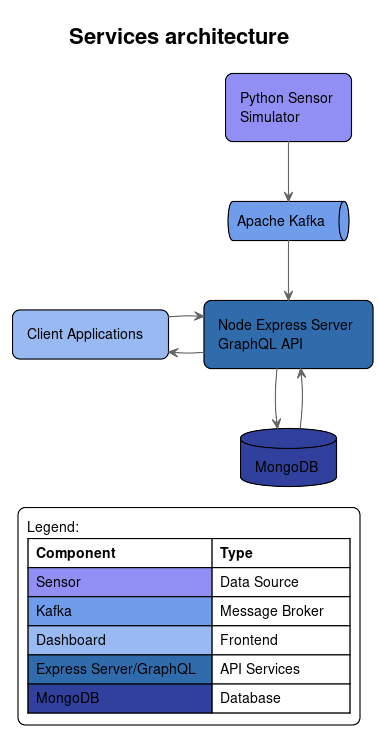
\includegraphics[width=0.5\textwidth]{architecture.png}
  \caption{Architettura generale del sistema}
  \label{fig:architecture}
\end{figure}

Di seguito vengono esplicitate le varie responsabilità per ognuno dei servizi precedentemente elencati.

\begin{itemize}
  \item Sensor service: questo servizio simula l'esercizio di un insieme di sensori, i quali registrano,
        con cadenza regolare, le misurazioni della qualità dell'aria. Ogni sensore è provvisto di un id univoco,
        un nome, una posizione geografica (le coordinate della sua collocazione) ed un indirizzo \acrshort{ip}.
        Tali misurazioni vengono inviate al broker dei messaggi in modo che vengano poi trasmesse ai servizi in ascolto.
  \item \acrshort{api} service: questo servizio consuma dal broker le misurazioni, le salva
        sul database non relazione e le rende disponibili attraverso \acrshort{api}.
  \item Dashboard service: questo servizio fornisce un'interfaccia grafica tramite cui è possibile consultare
        la mappa interattiva, aggiornata in tempo reale con i dati forniti dal server \acrshort{api}, e le relative
        tabelle.
\end{itemize}

\section{Sensor service}

In questa sezione verrà descritto il servizio che simula il sensore e la relativa generazione di misurazioni fittizie
sulla qualità dell'aria.

\subsection{Modello sensore}

Il sensore è dotato di un insieme di proprietà specifiche che ne determinano il funzionamento.
Queste proprietà sono:

\begin{itemize}
  \item Id (\texttt{sensor\_id}): stringa, identificatore univoco del sensore.
  \item Nome (\texttt{name}): stringa, nome del sensore.
  \item Posizione (\texttt{location}): oggetto, posizione in cui è collocato il sensore.
        Si tratta di un oggetto composto dal tipo (in questo caso \texttt{Point}) e dalle coordinate,
        longitudine e latitudine, ambo valori numerici a virgola mobile (\texttt{double}).
  \item \acrshort{ip} (\texttt{ip}): stringa, indirizzo ip del sensore.
  \item Attivo (\texttt{active}): booleano, indica se il sensore è attivo (\texttt{true})
        oppure no (\texttt{false}).
  \item Ultima misurazione (\texttt{last\_seen}): data, ultima volta che il sensore ha registrato una misurazione.
        \label{lst:sensors-properties}
\end{itemize}

\subsection{Generazione pseudo-misurazioni}

La classe \texttt{AirQualitySensor} è dotata di un metodo \texttt{generate\_reading} che produce misurazioni simulate.
Ad ogni sensore viene fornita la configurazione presentata nel listato~\ref{lst:sensor-config} per la generazione
delle misurazioni.

\begin{lstlisting}[caption={Configurazione sensore}, label=lst:sensor-config]
  SENSOR_CONFIG = {
    'sampling_rate': 10,            # seconds (def. 60)

    # Sensor ranges
    'temperature_range': (-15, 35), # Celsius degrees
    'humidity_range': (30, 100),    # %
    'pressure_range': (980, 1020),  # hPa
    'voc_range': (0, 3),            # ppm
    'co2_range': (400, 2000),       # ppm
    'pm25_range': (0, 150),         # micrograms/m^3
    'pm10_range': (0, 300),         # micrograms/m^3
    'no2_range': (0, 200),          # micrograms/m^3
    'o3_range': (0, 200),           # micrograms/m^3
    'so2_range': (0, 300),          # micrograms/m^3
  }
\end{lstlisting}

Per mantenere coerenza nei dati e evitare valori troppo discordanti, ogni nuova misurazione generata dal sensore
si basa sulla lettura precedente (quando disponibile) e si discosta da essa di una percentuale compresa tra
l'1\% e il 5\%.

Parte del codice Python utilizzato per la generazione di queste misurazioni simulate è riportato
nel listato~\ref{lst:generate-reading} che segue.

\begin{lstlisting}[caption={Metodo per la generazione di pseudo-misurazioni}, label=lst:generate-reading]
  def generate_reading(self):
    """Generate a realistic sensor reading with some correlation between values
    and small random changes (1-5%) from previous readings if available"""

    # Apply random change of 1-5% to previous values
    def random_change(value):
        percent_change = random.uniform(0.01, 0.05)  # 1-5%
        direction = random.choice([-1, 1])  # Increase or decrease
        return value * (1 + direction * percent_change)

    # Gas pollutants with random changes #

    # PM2.5 and PM10 with correlation maintained
    pm25 = random_change(self.last_reading['pm25'])
    pm25 = np.clip(pm25, *self.config['pm25_range'])

    pm10 = max(pm25 + random_change(self.last_reading['pm10'] - self.last_reading['pm25']), pm25)
    pm10 = np.clip(pm10, pm25, self.config['pm10_range'][1])

    # Nitrogen dioxide levels
    no2 = random_change(self.last_reading['no2'])
    no2 = np.clip(no2, *self.config['no2_range'])

    # Ozone levels
    o3 = random_change(self.last_reading['o3'])
    o3 = np.clip(o3, *self.config['o3_range'])

    # Sulfur dioxide levels
    so2 = random_change(self.last_reading['so2'])
    so2 = np.clip(so2, *self.config['so2_range'])
\end{lstlisting}

\subsection{Distribuzione sensori}
\label{subsection:sensor-distribution}

La scelta dei sensori è stata fatta relativamente ai punti di maggiore traffico, quali le intersezioni stradali
fra le arterie principali e le strade secondarie. Bologna presenta una moltitudine di semafori, luogo dove veicoli
fermi in attesa tendono a creare punti di maggiore concentrazione di inquinanti. Come anticipato precedentemente
con la query \ref{lst:overpass-query}, sono stati estrapolati tutti i punti che rappresentano un'intersezione
stradale di questo tipo. Data l'elevata densità di posizioni rilevate, è stata applicata una selezione sistematica
per mantenere un singolo punto per ogni intervallo di spazio regolare.
Questa selezione ha permesso anche di gestire le situazioni di affollamento, tipiche di rotonde,
nelle quali ogni svincolo è rappresentato come un incrocio, e di centri abitati, nei quali la concentrazione
di queste intersezioni risulta più elevato.

Nelle immagini \ref{fig:sensors-before} e \ref{fig:sensors-after} viene mostrato come, partendo da un dataset
consistente di punti, questi siano stati poi filtrati secondo i criteri precedentemente esposti.
È stata implementata una griglia di campionamento con spaziatura di 250 metri, parametro calibrato
sperimentalmente per ottenere una densità ottimale di punti. Per fare ciò è stata realizzata una pagina dedicata
allo scopo, dato che si tratta di un processo che può essere riprodotto
cambiando la distanza fra i punti tramite input numerico.
La pagina presenta una parte iniziale dove è possibile scegliere la città (nel nostro caso Bologna) e lo spazio
minimo fra un sensore e l'altro. Viene anche indicata la query di estrazione,
la stessa citata in precedenza nel listato~\ref{lst:overpass-query}.
Questa parte d'intestazione è riportata nell'immagine~\ref{fig:sensors-heading}, dove si possono notare gli elementi
citati.

\begin{figure}[H]
  \centering
  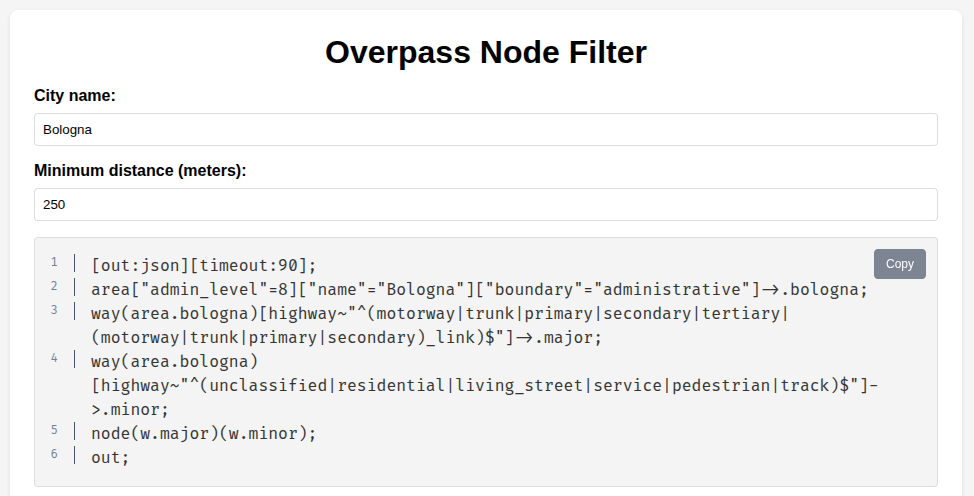
\includegraphics[width=\textwidth]{sensors/00_heading.png}
  \caption{Intestazione pagina}
  \label{fig:sensors-heading}
\end{figure}

Sotto di essa, è disponibile la mappa che mostra i nodi risultanti dalla query.
Tali nodi vengono disposti su 3 livelli, che sono: nodi originali, nodi filtrati e nodi differenza.
I primi, quelli originali (in rosso, immagine~\ref{fig:sensors-before}),
sono ottenuti direttamente dalla query ~\ref{formula:sensors-original}.
I secondi, quelli filtrati (in blu, immagine~\ref{fig:sensors-after}), sono il risultato del trattamento effettuato
su di essi, dato dall'elezione di un solo nodo ogni 250 metri ~\ref{formula:sensors-filtered}.
Gli ultimi infine, quelli di differenza (in verde, immagine~\ref{fig:sensors-difference}),
sono semplicemente i nodi originali
meno quelli filtrati ~\ref{formula:sensors-difference}.
La richiesta viene effettuata nel momento in cui viene cliccato il pulsante di invio, che riporta la
dicitura \textit{"Submit request"}. Si tratta di una chiamata POST
all'indirizzo \url{https://overpass-api.de/api/interpreter"}, il quale restituisce un \acrshort{json} in caso di
esito positivo.

\definecolor{sensors-original}{HTML}{e74c3c}
\definecolor{sensors-filtered}{HTML}{3498db}
\definecolor{sensors-difference}{HTML}{27ae60}

\begin{align}
  \textcolor{sensors-original}{O}   & = \text{insieme degli elementi originali} \label{formula:sensors-original}                                                                                                                            \\
  \textcolor{sensors-filtered}{F}   & = \text{sottoinsieme filtrato, dove } \textcolor{sensors-filtered}{F}\subseteq \textcolor{sensors-original}{O} \label{formula:sensors-filtered}                                                       \\
  \textcolor{sensors-difference}{D} & = \textcolor{sensors-original}{O} \setminus \textcolor{sensors-filtered}{F} = \{x \in \textcolor{sensors-original}{O} : x \notin \textcolor{sensors-filtered}{F}\} \label{formula:sensors-difference}
\end{align}

\newpage

\begin{figure}[H]
  \centering

  \begin{subfigure}{\textwidth}
    \centering
    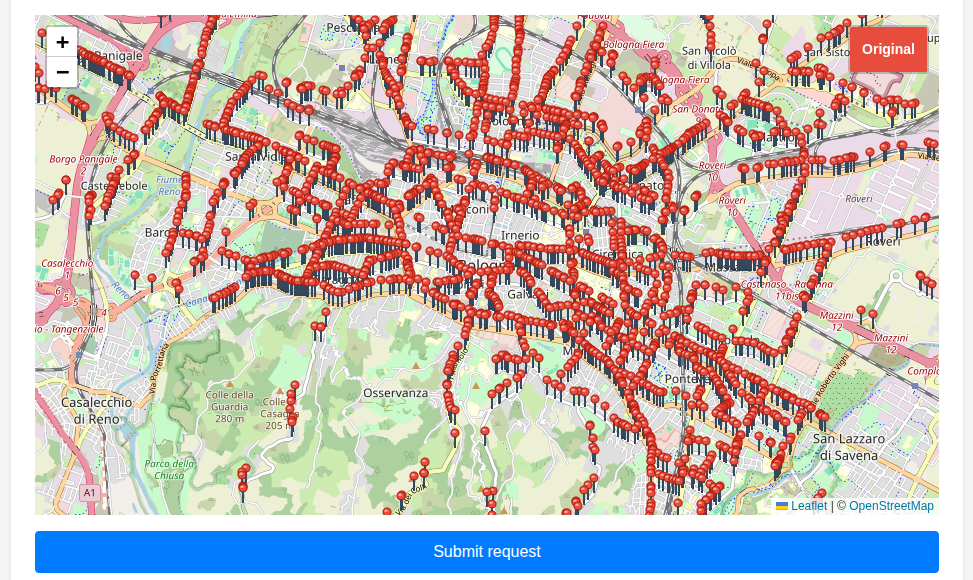
\includegraphics[width=0.85\textwidth]{sensors/01_original.png}
    \caption{Risultato originale della query}
    \label{fig:sensors-before}
  \end{subfigure}

  \hfill
  \begin{subfigure}{\textwidth}
    \centering
    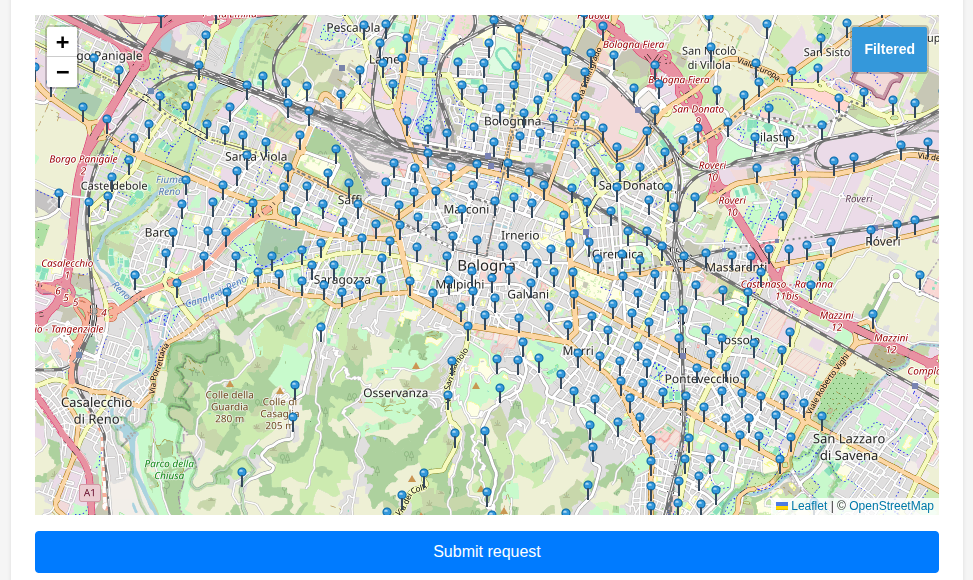
\includegraphics[width=0.85\textwidth]{sensors/02_filtered.png}
    \caption{Punti filtrati finali}
    \label{fig:sensors-after}
  \end{subfigure}

  \hfill
  \begin{subfigure}{\textwidth}
    \centering
    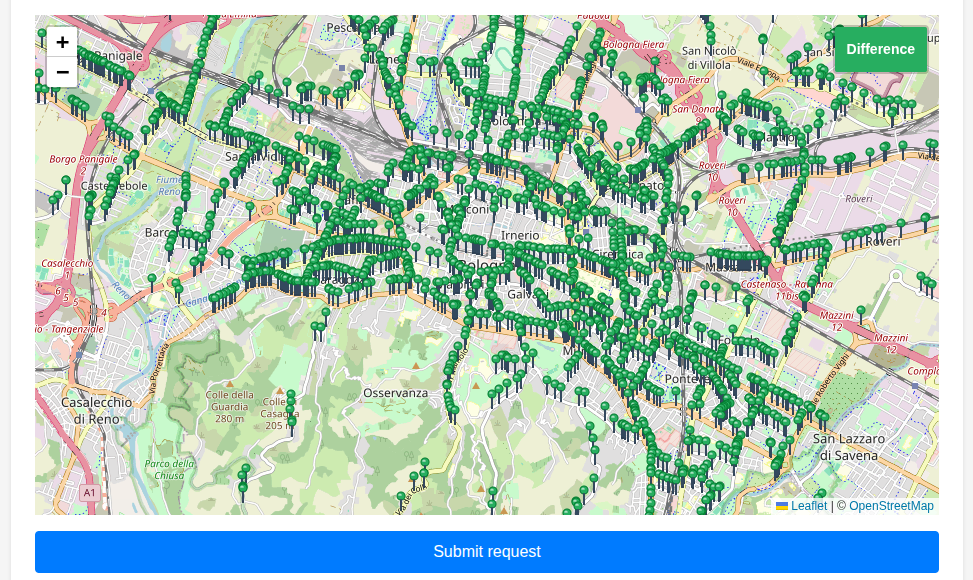
\includegraphics[width=0.85\textwidth]{sensors/03_difference.png}
    \caption{Punti di differenza}
    \label{fig:sensors-difference}
  \end{subfigure}

  \caption{Acquisizione punti delle intersezioni stradali}
\end{figure}

\newpage

Come ultimo elemento, la parte finale della pagina, esposta nell'immagine~\ref{fig:sensors-footer},
riporta le statistiche quali il numero di sensori originale,
il numero di sensori filtrati e la riduzione espressa come percentuale.
Premendo il pulsante con scritto \textit{"Download filtered \acrshort{json}"} è possibile scaricare il
\acrshort{json} dei sensori filtrati ottenuti. Tale \acrshort{json} presenta i sensori usati per popolare la mappa
dell'applicazione principale.

\begin{figure}[H]
  \centering
  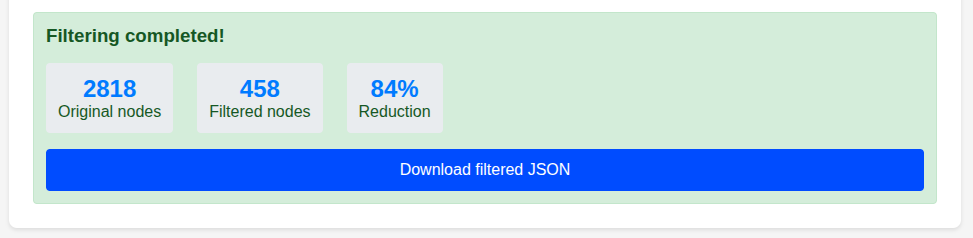
\includegraphics[width=\textwidth]{sensors/03_footer.png}
  \caption{Piè di pagina}
  \label{fig:sensors-footer}
\end{figure}

\section{\acrshort{api} service}

In questa sezione verrà descritto il servizio \acrshort{api} che riceve le misurazioni simulate della qualità dell'aria
dal broker di messaggi, le trasforma ed eroga ai client che lo interrogano.

\subsection{Implementazione del Server}

Il server Node.js fornisce un servizio web per la gestione e l'accesso ai dati delle misurazioni ambientali.
Utilizza Express.js per implementare un'interfaccia \acrshort{rest} che espone diversi endpoint per le operazioni sui dati.
Il server integra MongoDB per la memorizzazione persistente dei dati sensoriali, Apache Kafka per il consumo
continuo dei flussi di dati in arrivo dai sensori, e Socket.IO per fornire notifiche push in tempo reale ai client web
quando vengono registrate nuove misurazioni o superati i valori di soglia configurati. La configurazione \acrshort{cors}
permette l'accesso sicuro da domini diversi, consentendo l'integrazione con applicazioni web distribuite.

\subsection{Endpoint Disponibili}

Di seguito verranno elencati gli endpoint disponibili esposti dalle \acrshort{api}.
Tutti gli endpoint di seguito elencati restituiscono un \acrshort{json} ed un codice di stato \acrshort{http} che può
essere \texttt{200 OK} in caso di successo o \texttt{500 Internal Server Error} in caso di errore.

\paragraph{Health Check - \texttt{GET /health}}

Endpoint per il monitoraggio dello stato del servizio.
Verifica la disponibilità del server e restituisce lo stato operativo.
Risponde con un semplice \acrshort{json} con lo status, il tempo di attività, il numero di sensori attivi e le
misurazioni registrate come da esempio nel listato~\ref{lst:api-health-example}.

\begin{lstlisting}[caption={Risposta di sucesso per endpoint \texttt{health}}, label=lst:api-health-example]
  {
    "status":"healthy",
    "timestamp":"2025-08-30T13:58:44.198Z",
    "uptime":39.198012656,
    "wot_things":459,
    "active_measurements":258
  }
\end{lstlisting}

\paragraph{Recupero Misurazioni - \texttt{GET /api/measurements}}

Endpoint per il recupero delle misurazioni ambientali con supporto per filtri e paginazione.
Restituisce le misurazioni archiviate nel database con possibilità di filtraggio per sensore e intervallo temporale.

È possibile utilizzare dei parametri opzionali di query, quali
\texttt{sensorId} come identificativo del sensore specifico,
data di inizio \texttt{startDate} e fine \texttt{endDate} del periodo di misurazione (in formato \acrshort{iso} 8601).
Se specificato \texttt{sensorId}, filtra per sensore specifico,
mentre se specificati \texttt{startDate} e \texttt{endDate}, filtra per intervallo temporale.
Le misurazioni in risposta sono in ordine crescente per timestamp e con limite massimo di 1000 record per richiesta.

Un esempio di risposta di successo è riportato nel listato~\ref{lst:api-measurements-example}
\begin{lstlisting}[caption={Risposta di sucesso per endpoint \texttt{measurements}},label=lst:api-measurements-example]
[
  {
    "_id":"68a4def8c82270d8766481f6",
    "sensor_id":"SENSOR00436",
    "timestamp":"2025-08-19T22:30:48.494Z",
    "temperature":2.64,
    "humidity":75.87,
    "pressure":1019.63,
    "voc":0.647,
    "co2":400,"pm25":55.43,
    "pm10":177.75,
    "no2":132.4,
    "o3":65.45,
    "so2":35.95,
    "__v":0
  },
  ...
]
\end{lstlisting}

\paragraph{Lista Sensori - \texttt{GET /api/sensors}}

Endpoint per il recupero dell'elenco completo dei sensori registrati nel sistema.
Restituisce tutti i sensori configurati con le relative informazioni di localizzazione e configurazione.
È possibile utilizzare come parametro opzionale di query \texttt{sensorId} come identificativo del sensore specifico,
estraendo il solo sensore indicato (se disponibile).

Un esempio di risposta di successo è riportato nel listato~\ref{lst:api-sensors-example}
\begin{lstlisting}[caption={Risposta di sucesso per endpoint \texttt{sensors}},label=lst:api-sensors-example]
[
  {
    "location": { "type": "Point", "coordinates": [11.3482468, 44.4856545] },
    "_id": "68a4b0b50bb78efcdfbaa8b9",
    "sensor_id": "SENSOR00001",
    "name": "d0d54bf349674398",
    "ip": "192.168.0.1",
    "active": true,
    "last_seen": "2025-08-30T10:21:32.252Z"
  },
  ...
]
\end{lstlisting}

\paragraph{Ultima Misurazione - \texttt{GET /api/latest}}

Endpoint per il recupero della misurazione più recente nel sistema.
Restituisce l'ultima misurazione registrata, ordinata per timestamp decrescente.

Un esempio di risposta di successo è riportato nel listato~\ref{lst:api-latest-example}
\begin{lstlisting}[caption={Risposta di sucesso per endpoint \texttt{latest}},label=lst:api-latest-example]
{
  "_id":"68b421c342b53a3e45108d73",
  "sensor_id":"SENSOR00238",
  "timestamp":"2025-08-30T12:19:47.467Z",
  "temperature":15.42,
  "humidity":32.71,
  "pressure":980,
  "voc":1.937,
  "co2":417.1,
  "pm25":16.76,
  "pm10":131.12,
  "no2":57.75,
  "o3":130.33,
  "so2":112.44,
  "__v":0
}
\end{lstlisting}

\paragraph{Directory WoT - \texttt{GET /wot/things}}

Endpoint per il discovery automatico dei dispositivi registrati nel gateway.
Restituisce un elenco di tutti i Thing disponibili con informazioni sommarie su identità,
stato operativo e ultimo contatto. Supporta la notifica proattiva via WebSocket per mantenere sincronizzate
le applicazioni client senza polling periodico.

Un esempio di risposta di successo è riportato nel listato~\ref{lst:wot-directory-example}
\begin{lstlisting}[caption={Risposta di successo per endpoint \texttt{/wot/things}}, label=lst:wot-directory-example]
[
  {
    "id": "SENSOR00001",
    "title": "d0d54bf349674398",
    "description": "Air Quality Sensor monitoring environmental parameters at 11.3482468,44.4856545",
    "base": "http://localhost:3000/wot/things/SENSOR00001",
    "status": "active",
    "lastContact": "2025-08-30T10:21:32.252Z",
    "properties": [
      "temperature",
      "humidity",
      "pressure",
      "voc",
      "co2",
      "pm25",
      "pm10",
      "no2",
      "o3",
      "so2",
      "status",
      "location"
    ],
    "actions": ["getLatestMeasurement"]
  },
  ...
]
\end{lstlisting}

\paragraph{\acrlong{td} - \texttt{GET /wot/things/\{sensorId\}}}

Endpoint per il recupero della \acrlong{td} completa per un sensore specifico.
Restituisce la TD conforme alla specifica \acrshort{w3c} \acrshort{wot} \acrshort{td} v1.1, includendo il contesto
semantico, le proprietà disponibili, le azioni supportate e tutti i metadati del dispositivo.
La risposta contiene l'intera struttura \acrshort{json} della \acrlong{td} con vocabolari \acrlong{saref} e definizioni
complete delle forme di interazione.

Un esempio di risposta di successo è riportato nel listato~\ref{lst:wot-thing-example}
\begin{lstlisting}[caption={Risposta di successo per endpoint \texttt{/wot/things/{sensorId}}}, label=lst:wot-thing-example]
{
  "@context": [
    "https://www.w3.org/2022/wot/td/v1.1",
    { "saref": "https://saref.etsi.org/core/" }
  ],
  "@type": ["Thing", "saref:Sensor"],
  "id": "urn:sensor:air-quality:SENSOR00001",
  "title": "d0d54bf349674398",
  "description": "Air Quality Sensor monitoring environmental parameters at 11.3482468,44.4856545",
  "base": "http://localhost:3000/wot/things/SENSOR00001",
  "securityDefinitions": { "nosec_sc": { "scheme": "nosec" } },
  "security": ["nosec_sc"],
  "properties": {
    "temperature": {
      "type": "number",
      "title": "Temperature",
      "description": "Ambient temperature in Celsius",
      "unit": "Celsius degrees",
      "minimum": -15,
      "maximum": 35,
      "readOnly": true,
      "observable": false,
      "forms": [
        {
          "href": "http://localhost:3000/wot/things/SENSOR00001/properties/temperature",
          "contentType": "application/json",
          "op": ["readproperty"]
        }
      ]
    },
    "humidity": {...},
    "pressure": {...},
    "voc": {...},
    "co2": {...},
    "pm25": {...},
    "pm10": {...},
    "no2": {...},
    "o3": {...},
    "so2": {...},
    "status": {
      "type": "string",
      "title": "Status",
      "description": "Current sensor status",
      "enum": ["active", "inactive"],
      "readOnly": true,
      "observable": false,
      "forms": [
        {
          "href": "http://localhost:3000/wot/things/SENSOR00001/properties/status",
          "contentType": "application/json",
          "op": ["readproperty"]
        }
      ]
    },
    "location": {
      "type": "object",
      "title": "Location",
      "description": "Sensor geographical location",
      "properties": {
        "latitude": { "type": "number" },
        "longitude": { "type": "number" }
      },
      "readOnly": true,
      "observable": false,
      "forms": [
        {
          "href": "http://localhost:3000/wot/things/SENSOR00001/properties/location",
          "contentType": "application/json",
          "op": ["readproperty"]
        }
      ]
    }
  },
  "actions": {
    "getLatestMeasurement": {
      "title": "Get Latest Measurement",
      "description": "Get the latest complete measurement from this sensor",
      "forms": [
        {
          "href": "http://localhost:3000/wot/things/SENSOR00001/actions/getLatestMeasurement",
          "contentType": "application/json",
          "op": ["invokeaction"]
        }
      ]
    }
  }
}
\end{lstlisting}

\paragraph{Proprietà Singola - \texttt{GET /wot/things/\{sensorId\}/properties/\{propertyName\}}}

Endpoint per l'accesso alle singole proprietà del Thing.
Restituisce il valore corrente della proprietà richiesta incapsulato in un oggetto \acrshort{json} standardizzato.
Supporta tutte le proprietà ambientali (\texttt{temperature}, \texttt{humidity}, \texttt{pressure}, \texttt{voc},
\texttt{co2}, \texttt{pm25}, \texttt{pm10}, \texttt{no2}, \texttt{o3}, \texttt{so2}) oltre a proprietà di sistema
(\texttt{status}, \texttt{location}).

Un esempio di risposta di successo per la proprietà \texttt{temperature} è riportato
nel listato~\ref{lst:wot-property-example}
\begin{lstlisting}[caption={Risposta di successo per proprietà singola}, label=lst:wot-property-example]
{
  "value": 23.5
}
\end{lstlisting}

\paragraph{Tutte le Proprietà - \texttt{GET /wot/things/\{sensorId\}/properties}}

Endpoint per il recupero di tutte le proprietà del Thing in una singola chiamata.
Ottimizza l'efficienza della comunicazione permettendo di recuperare lo stato completo del sensore senza multiple
richieste \acrshort{http}. Restituisce un oggetto \acrshort{json} contenente tutte le proprietà con i relativi
valori correnti.

Un esempio di risposta di successo è riportato nel listato~\ref{lst:wot-properties-example}
\begin{lstlisting}[caption={Risposta di successo per tutte le proprietà}, label=lst:wot-properties-example]
{
  "temperature": { "value": -7.15 },
  "humidity": { "value": 54.52 },
  "pressure": { "value": 1020 },
  "voc": { "value": 1.71 },
  "co2": { "value": 431.7 },
  "pm25": { "value": 36.91 },
  "pm10": { "value": 90.61 },
  "no2": { "value": 133.43 },
  "o3": { "value": 54.66 },
  "so2": { "value": 270.31 },
  "status": { "value": "active" },
  "location": { "value": { "latitude": 11.3482468, "longitude": 44.4856545 } }
}
\end{lstlisting}

\paragraph{Invocazione Azioni - \texttt{GET /wot/things/\{sensorId\}/actions/\{actionName\}}}

Endpoint per l'invocazione delle azioni definite nella \acrlong{td}.
Attualmente supporta l'azione \texttt{getLatestMeasurement} che restituisce l'insieme completo delle misurazioni
più recenti del sensore. L'azione viene eseguita immediatamente e restituisce il risultato in formato \acrshort{json}
strutturato con tutti i parametri ambientali misurati.

Un esempio di risposta di successo per l'azione \texttt{getLatestMeasurement} è riportato
nel listato~\ref{lst:wot-action-example}
\begin{lstlisting}[caption={Risposta di successo per azione \texttt{getLatestMeasurement}},
  label=lst:wot-action-example]
{
  "result": {
    "sensor_id": "SENSOR00001",
    "timestamp": "2025-08-30T10:21:39.092Z",
    "temperature": -6.74,
    "humidity": 55.31,
    "pressure": 1020,
    "voc": 1.791,
    "co2": 421.9,
    "pm25": 35.67,
    "pm10": 89.71,
    "no2": 129.49,
    "o3": 56.53,
    "so2": 286.01
  }
}

\end{lstlisting}

\section{Dashboard service}

Questa sezione sarà dedicata alla descrizione dell'applicazione frontend sviluppata per il progetto AirQualityInsight.
L'esposizione verrà articolata in due parti distinte: nella prima sottosezione verrà presentata
l'interfaccia utente e verranno illustrate le scelte progettuali che hanno guidato la definizione del design,
mentre nella seconda sottosezione verrà fornita una descrizione dettagliata dell'implementazione
tecnica dell'applicazione.

\subsection{Design e architettura dell'interfaccia}

In questa sottosezione verrà illustrata l'interfaccia dell'applicazione e verranno esaminate le scelte progettuali
che hanno determinato la sua configurazione.
La progettazione dell'interfaccia è stata condotta tenendo conto degli obiettivi e delle funzionalità stabilite
durante la fase di analisi, nonché dello studio dello stato dell'arte delle applicazioni attualmente
disponibili nel settore.
Il processo di design dell'interfaccia grafica è stato orientato dai seguenti principi guida:
\begin{itemize}
  \item i requisiti funzionali e non funzionali definiti rispettivamente nelle sottosezioni
        \ref{subsec:requisiti-funzionali} e \ref{subsec:requisiti-non-funzionali}
  \item l'approccio mobile-first
  \item l'adozione del principio KISS, orientando l'interfaccia verso uno stile minimalista che privilegia strumenti
        di comunicazione non testuali, quali icone, elementi cromatici e simboli grafici
  \item l'analisi dello stato dell'arte delle applicazioni per il monitoraggio della qualità dell'aria,
        riportata nel capitolo \ref{chapter:first}: si è scelto di mantenere continuità
        con le applicazioni esistenti per il monitoraggio della qualità dell'aria, al fine di offrire agli utenti
        un'esperienza familiare e sfruttare le soluzioni progettuali già consolidate
\end{itemize}
L'architettura dell'interfaccia è stata strutturata mediante la suddivisione dei componenti
in tre categorie principali, classificate in base alla loro collocazione spaziale e alle rispettive funzionalità,
sia individuali che sinergiche con gli altri elementi del sistema.
Nei paragrafi seguenti verranno presentate le categorie identificate e i rispettivi componenti costitutivi.

\subsection{Implementazione}

In questa sottosezione verrà approfondita nel dettaglio l'implementazione dell'applicazione web di AirQualityInsight.
Tale applicazione è stata realizzata basandosi principalmente su Vue e Leaflet.
Nelle seguenti sottosezioni verranno esaminati i componenti dell'applicativo, ognuno dei quali fa riferimento
ad una porzione dell'interfaccia utente.

\paragraph{Intestazione}

La prima parte dell'applicazione web fornisce un'introduzione riguardo lo scopo del progetto e le sue funzionalità.
Nella seguenti immagini, vengono presentate all'utente, dall'alto verso il basso,
una breve descrizione \ref{fig:app-description},
la tabella relativa ai criteri di valutazione della qualità dell'aria \ref{fig:app-eaqi-table},
una guida sintetica sull'utilizzo della pagina \ref{fig:app-guide} ed infine
il metodo di calcolo utilizzato per ottenere l'\acrfull{eaqi} \ref{fig:app-eaqi-calculation}.

\begin{figure}[H]
  \centering
  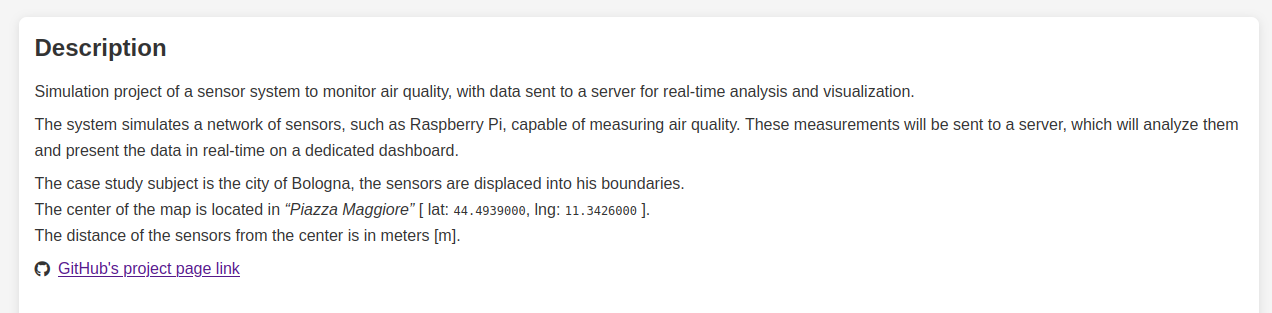
\includegraphics[width=\textwidth]{dashboard/00_disclaimer_description.png}
  \caption{Descrizione}
  \label{fig:app-description}
\end{figure}

\begin{figure}[H]
  \centering
  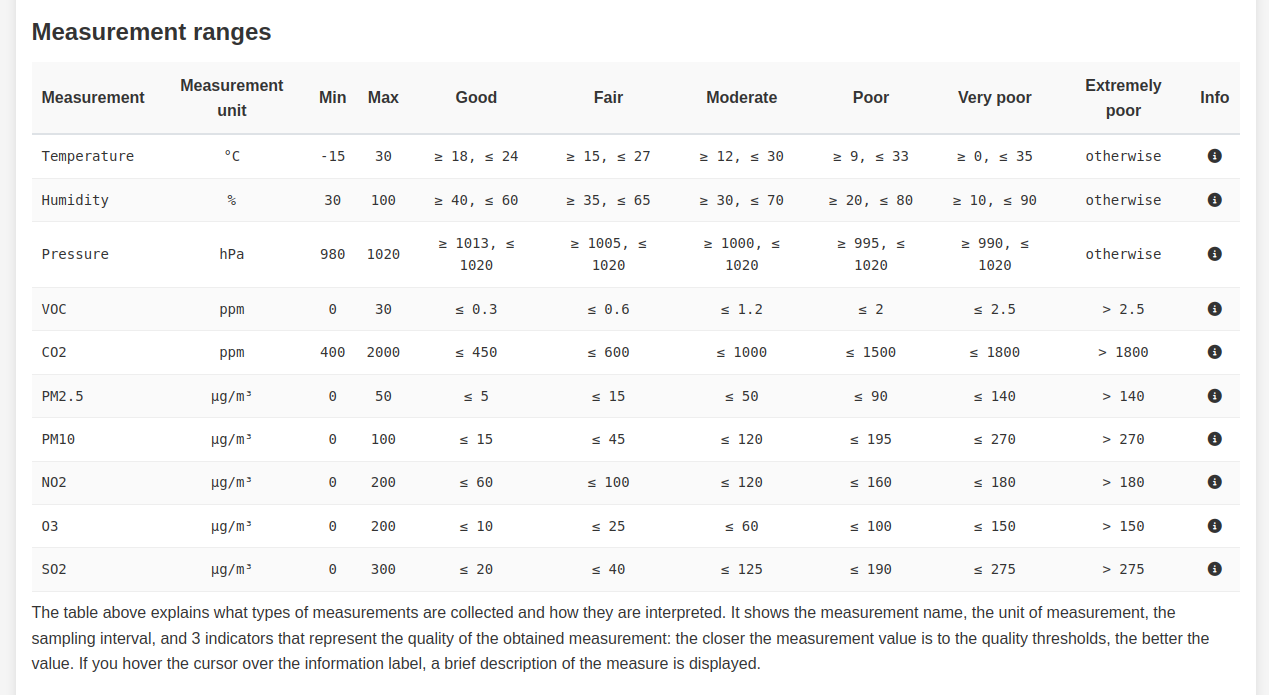
\includegraphics[width=\textwidth]{dashboard/01_table_measurement_ranges.png}
  \caption{Tabella valori riferimento \acrfull{eaqi}}
  \label{fig:app-eaqi-table}
\end{figure}

\begin{figure}[H]
  \centering
  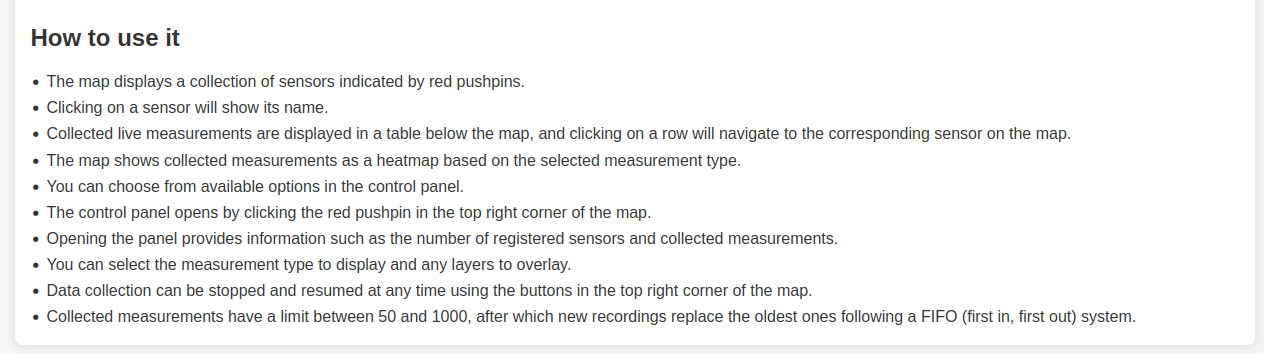
\includegraphics[width=\textwidth]{dashboard/02_disclaimer_how_to_use_it.png}
  \caption{Guida}
  \label{fig:app-guide}
\end{figure}

\begin{figure}[H]
  \centering
  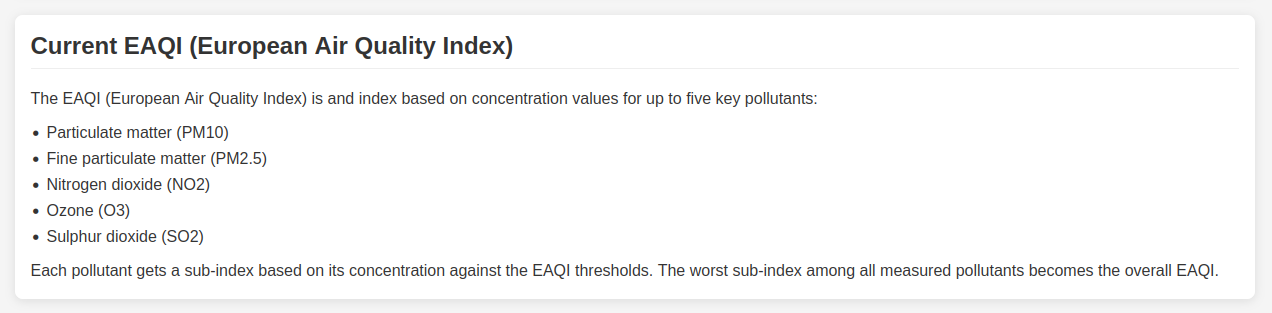
\includegraphics[width=\linewidth]{dashboard/03_disclaimer_eaqi.png}
  \caption{Calcolo \acrfull{eaqi}}
  \label{fig:app-eaqi-calculation}
\end{figure}

\paragraph{Mappa}

Accedendo alla pagina principale, l'utente si trova di fronte a una mappa dettagliata della città di Bologna,
come documentato nell'immagine \ref{fig:app-map-sensors}. I sensori attivi sul territorio
sono contrassegnati da spilli rossi, mentre il centro della mappa (Piazza Maggiore) è evidenziato da uno spillo blu
come si può osservare nell'immagine \ref{fig:app-map-center}. Nel momento in cui viene ricevuta una nuova misurazione,
il sensore responsabile viene lampeggia per un paio di secondi.

\begin{figure}
  \centering
  \begin{subfigure}{\textwidth}
    \centering
    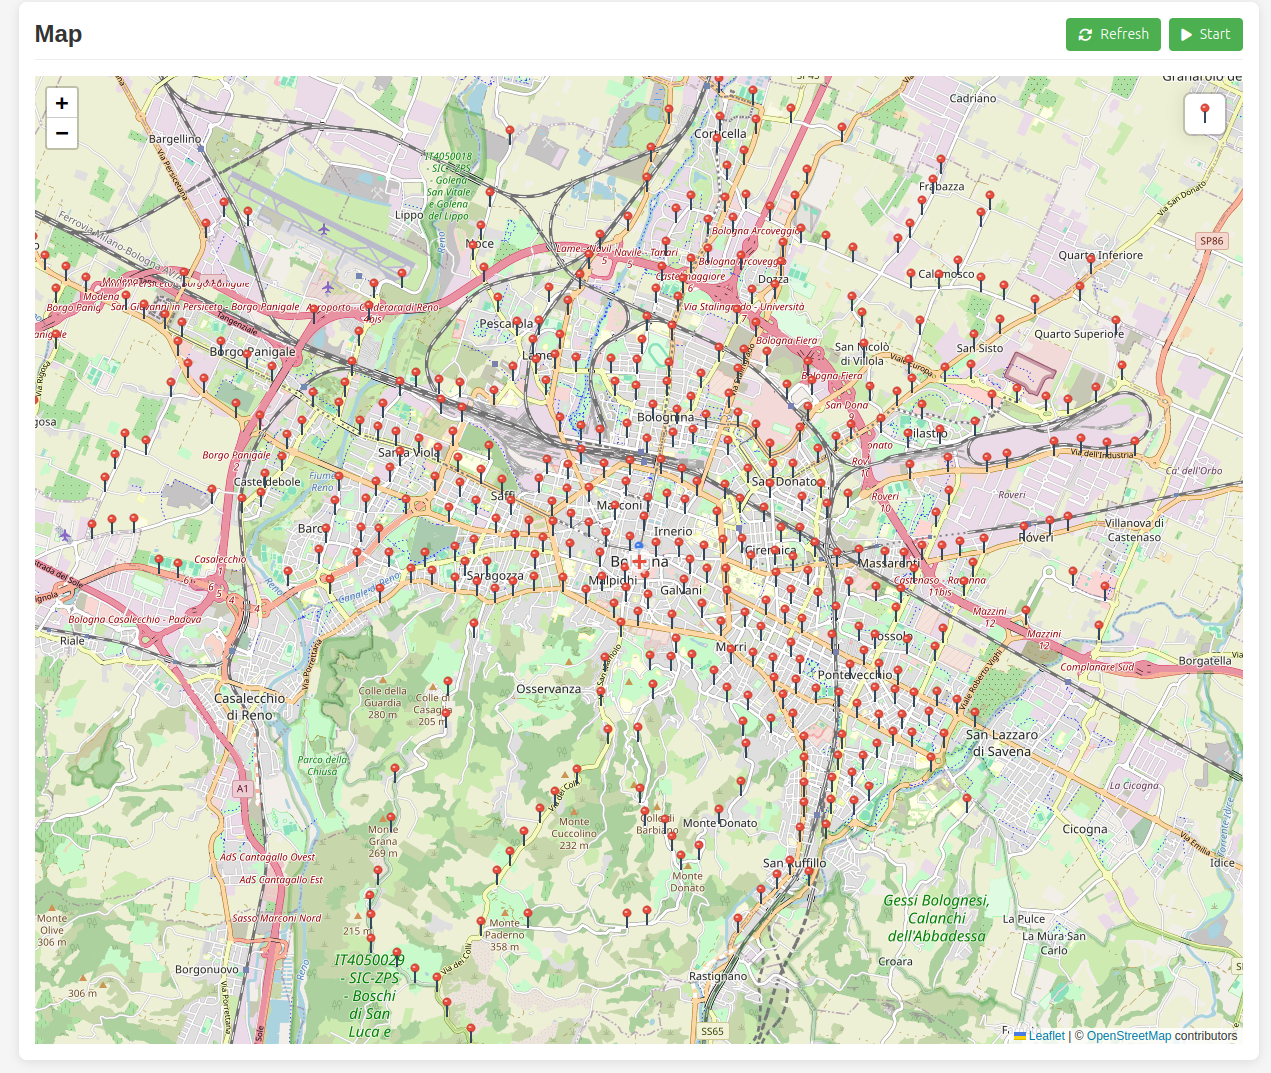
\includegraphics[width=0.95\textwidth]{dashboard/04_map_sensors.png}
    \caption{Mappa principale}
    \label{fig:app-map-sensors}
  \end{subfigure}

  \hfil
  \begin{subfigure}{\textwidth}
    \centering
    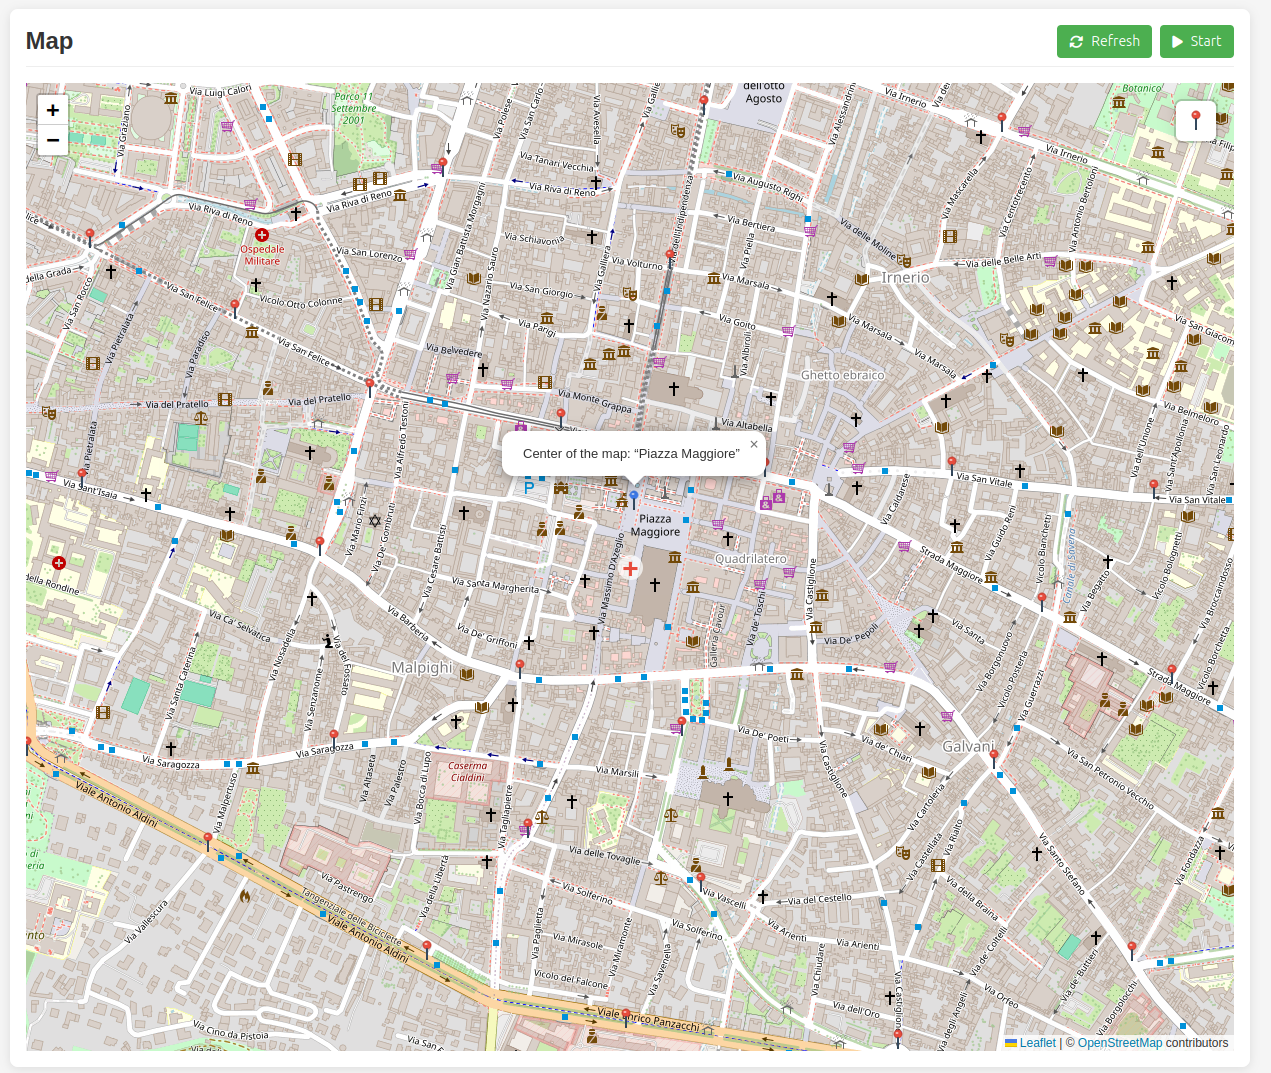
\includegraphics[width=0.95\textwidth]{dashboard/05_map_sensors_center_of_the_map.png}
    \caption{Centro della mappa}
    \label{fig:app-map-center}
  \end{subfigure}

  \caption{Mappa}
  \label{fig:app-map}
\end{figure}

L'interfaccia cartografica è dotata di diversi controlli interattivi: sul lato sinistro sono posizionati i pulsanti
per aumentare o diminuire lo zoom (\texttt{+} e \texttt{-}) della mappa, mentre sul lato destro si trovano due pulsanti
verdi ed uno bianco avente come icona uno spillo rosso.

Al centro della mappa è presente un mirino a croce (\textit{crosshair}) rosso dentro una cornice circolare bianca,
che indica il centro della mappa attualmente visualizzata. Il sistema registra automaticamente le coordinate geografiche
ad esso, conservandole in memoria e rendendole disponibili per la consultazione. Quando l'utente naviga sulla mappa
spostando la visualizzazione, le coordinate del punto centrale vengono aggiornate per mantenere la corrispondenza
con la nuova area geografica inquadrata.

Il pulsante verde contrassegnato dalla dicitura \textit{"Start"} rappresenta l'interruttore principale
per attivare o disattivare la ricezione in tempo reale delle misurazioni dai sensori.
All'avvio dell'applicazione, questa funzionalità risulta disabilitata per impostazione predefinita.
Una volta attivata, il sistema inizierà a visualizzare graficamente sulla mappa
i valori ricevuti dai sensori e aggiornerà automaticamente le tabelle informative sottostanti,
come documentato nelle figure \ref{fig:app-tab-last-measurements}, \ref{fig:app-tab-statistics},
\ref{fig:app-tab-system-log} e \ref{fig:app-tab-registered-sensors}.

Il pulsante avente come icona lo spillo rosso attiva l'espansione di un pannello di controllo che fornisce informazioni
dettagliate sulla mappa e strumenti aggiuntivi per l'interazione con l'interfaccia cartografica, come mostrato nelle
figure \ref{fig:map-layer-sensors} e \ref{fig:map-layer-clear}.

Procedendo dall'alto verso il basso, la prima informazione visualizzata concerne il conteggio complessivo
di tutti i sensori presenti sulla mappa, indipendentemente dal loro stato.
La sezione successiva presenta un pulsante verde dedicato alla copia delle coordinate geografiche del centro mappa
(corrispondenti alla posizione del mirino). Seguono una serie di pulsanti grigi che consentono
di attivare o disattivare la visualizzazione dei diversi layer cartografici: sensori, demarcazioni territoriali
come le zone di avviamento postale (\acrshort{cap}) (figura~\ref{fig:map-layer-caps}),
quartieri (figura~\ref{fig:map-layer-neighborhoods}),
zone amministrative (figura~\ref{fig:map-layer-zones}) e \acrshort{ztl} (figura~\ref{fig:map-layer-ztl}).

Nella parte inferiore del pannello si trovano un menu a tendina per la selezione del tipo di inquinante da visualizzare,
uno slider orizzontale per impostare il numero di misurazioni da registrare (range da 50 a 1000),
un indicatore del numero di misurazioni attualmente memorizzate e un pulsante rosso con icona cestino per
l'eliminazione dei dati registrati. Il sistema implementa un meccanismo di registrazione delle misurazioni dei sensori
basato su una coda (struttura dati \acrshort{fifo}), che garantisce l'eliminazione automatica delle registrazioni
più datate quando viene raggiunta la capacità massima prestabilita, conservando i dati più recenti.

Conclude l'interfaccia un menu a tendina aggiuntivo per l'attivazione di griglie di riferimento sulla mappa
quali una grigia (figura~\ref{fig:map-grid-gray}), una rossa
(figura~\ref{fig:map-grid-red}) ed una grigia crosshair che divide la mappa
in quattro quarti (figura~\ref{fig:map-grid-crosshair}).

\begin{figure}[H]
  \centering

  \begin{subfigure}{0.48\textwidth}
    \centering
    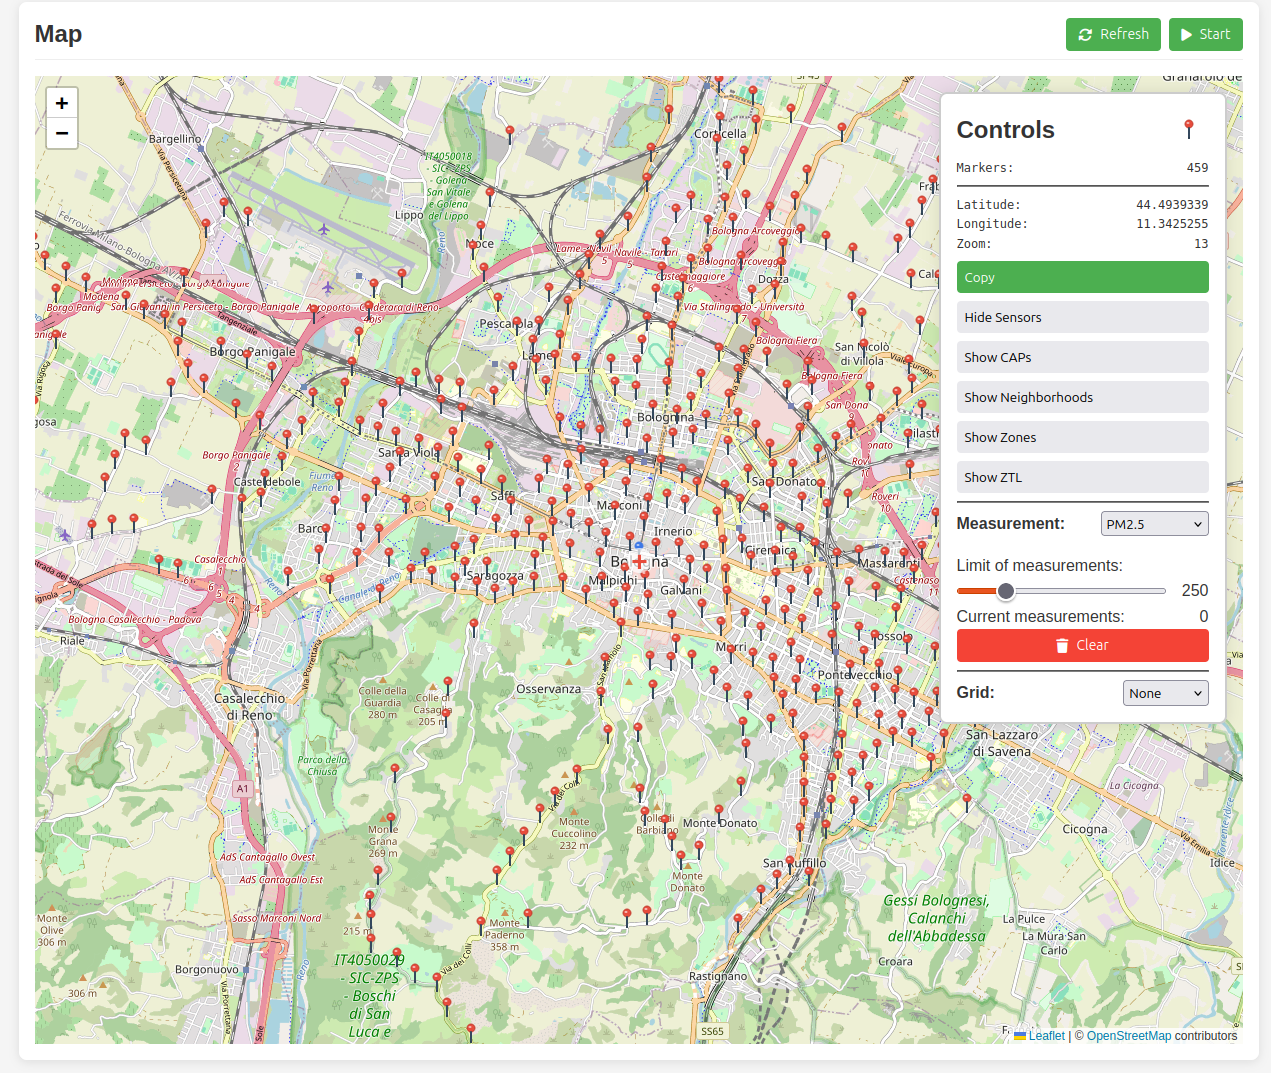
\includegraphics[width=\textwidth]{dashboard/06_map_sensors_controls.png}
    \caption{Pannello controllo espanso con sensori visualizzati}
    \label{fig:map-layer-sensors}
  \end{subfigure}
  \hfill
  \begin{subfigure}{0.48\textwidth}
    \centering
    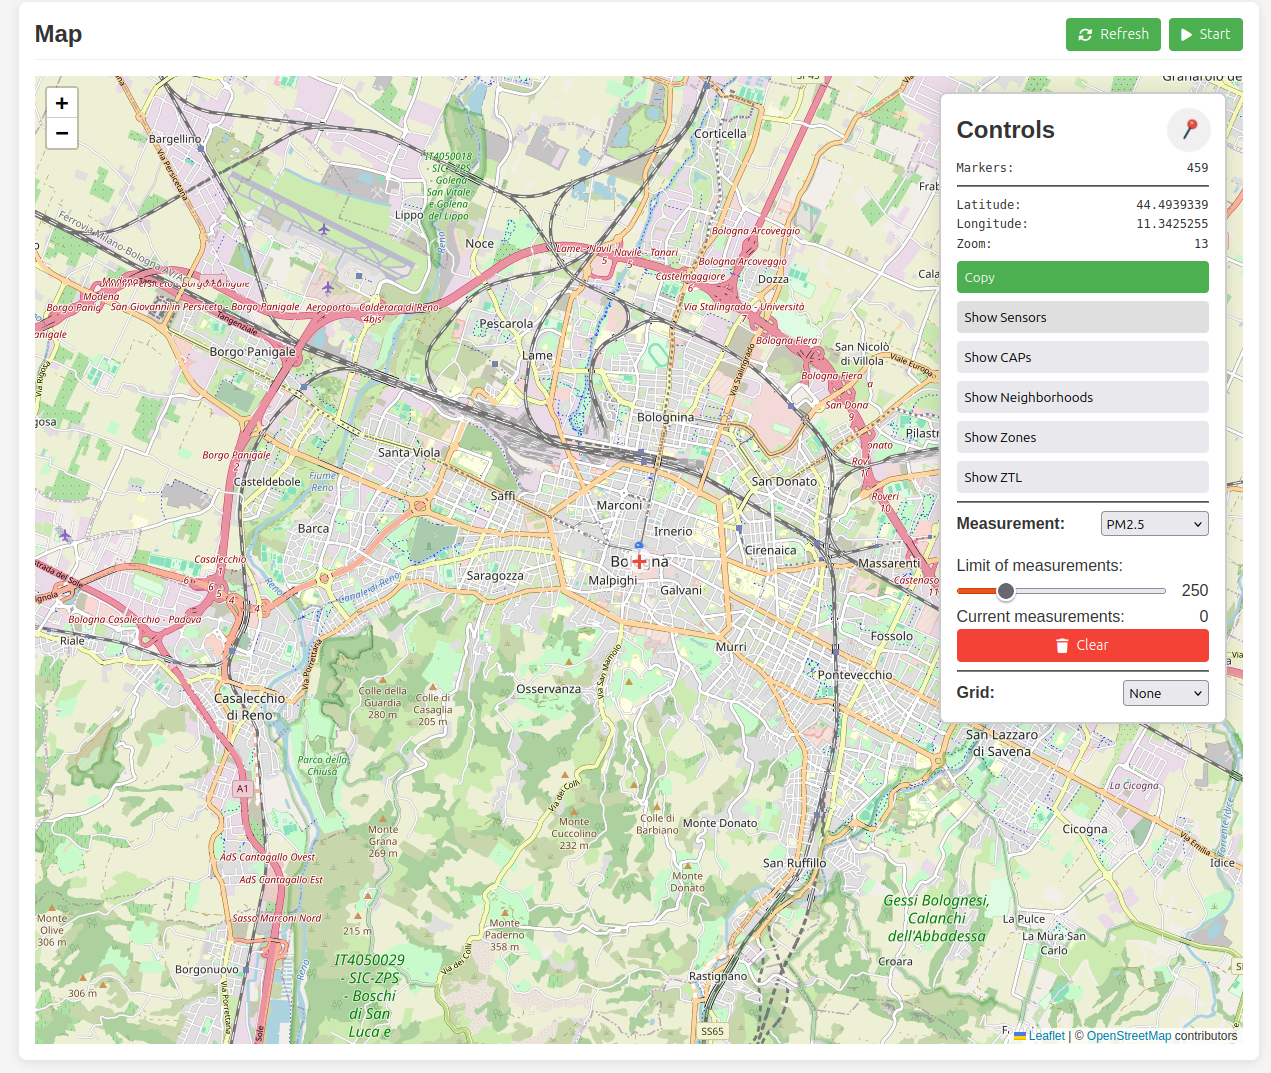
\includegraphics[width=\textwidth]{dashboard/07_map_controls.png}
    \caption{Pannello controllo espanso con sensori nascosti}
    \label{fig:map-layer-clear}
  \end{subfigure}

  \vspace{1em}

  \begin{subfigure}{0.48\textwidth}
    \centering
    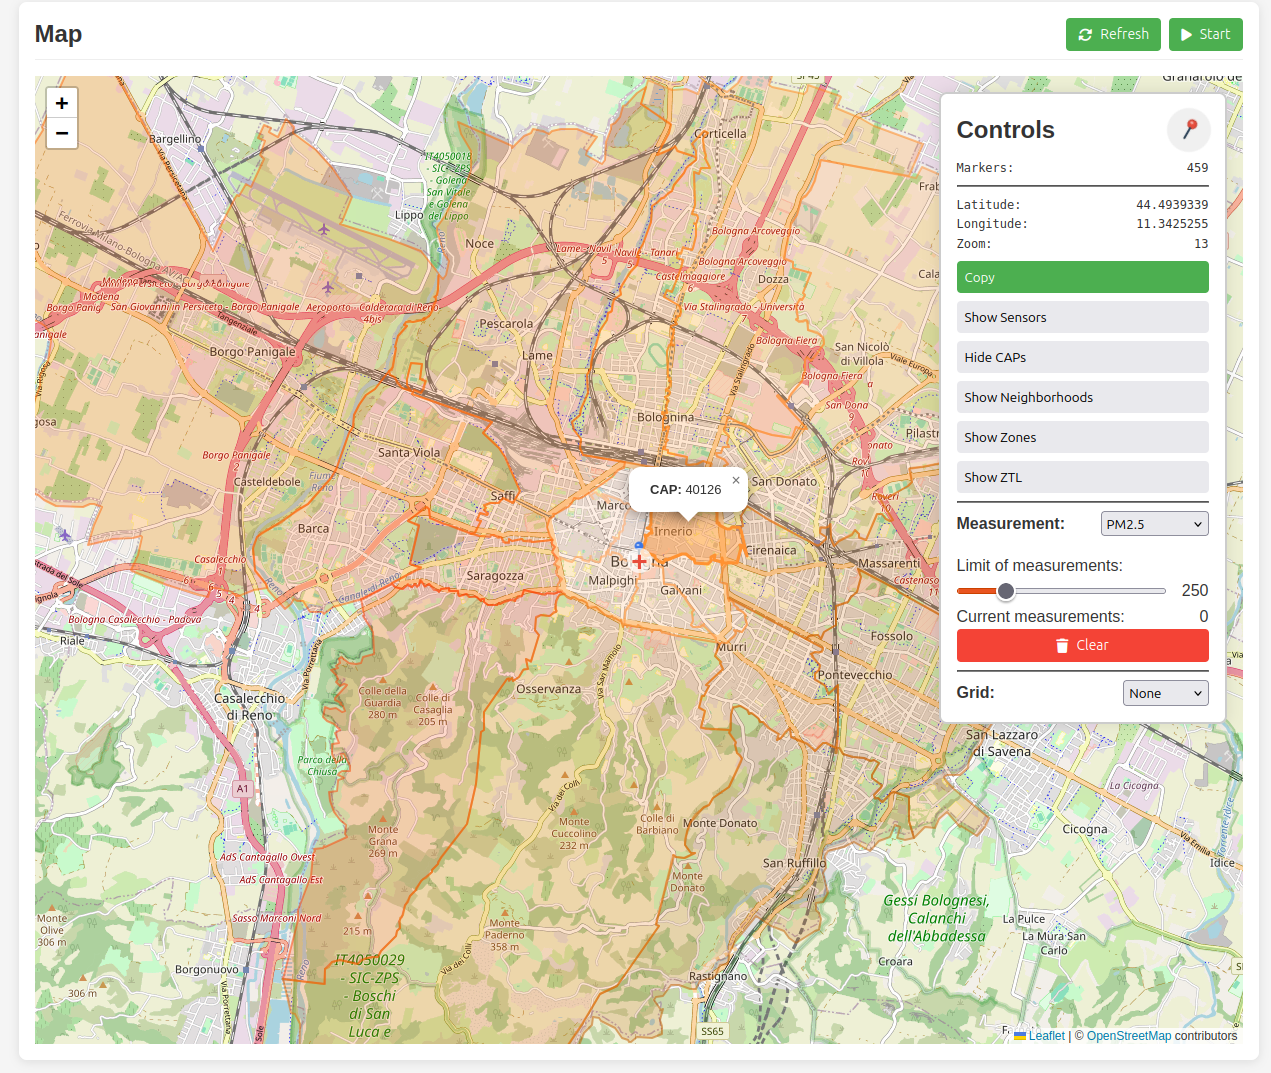
\includegraphics[width=\textwidth]{dashboard/08_map_caps_controls.png}
    \caption{Livello a \acrshort{cap}}
    \label{fig:map-layer-caps}
  \end{subfigure}
  \hfill
  \begin{subfigure}{0.48\textwidth}
    \centering
    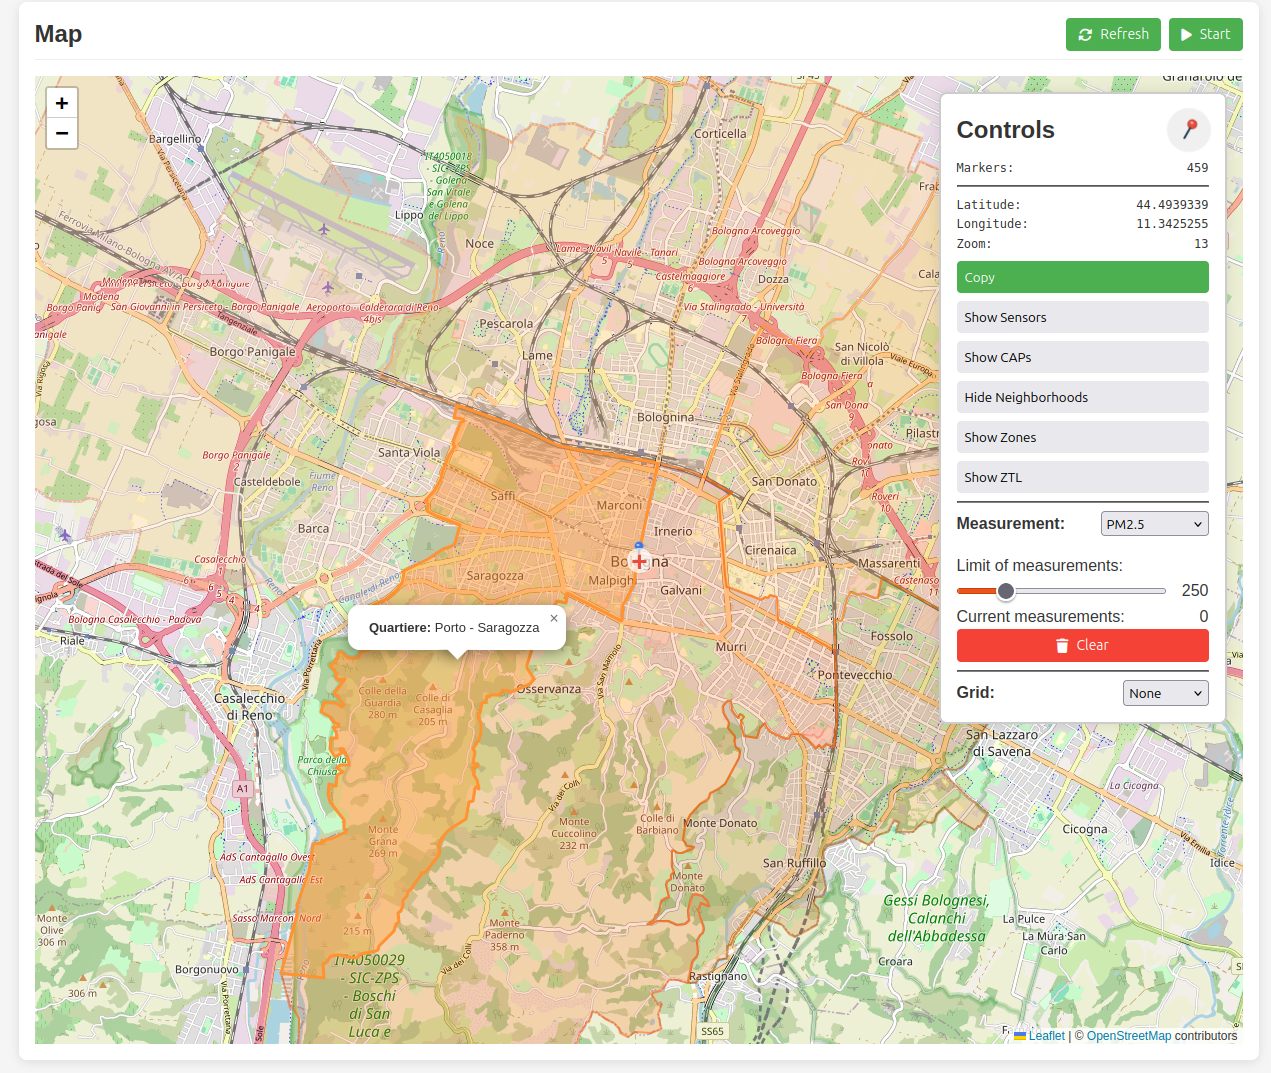
\includegraphics[width=\textwidth]{dashboard/09_map_neighborhoods_controls.png}
    \caption{Livello a quartieri}
    \label{fig:map-layer-neighborhoods}
  \end{subfigure}

  \vspace{1em}

  \begin{subfigure}{0.48\textwidth}
    \centering
    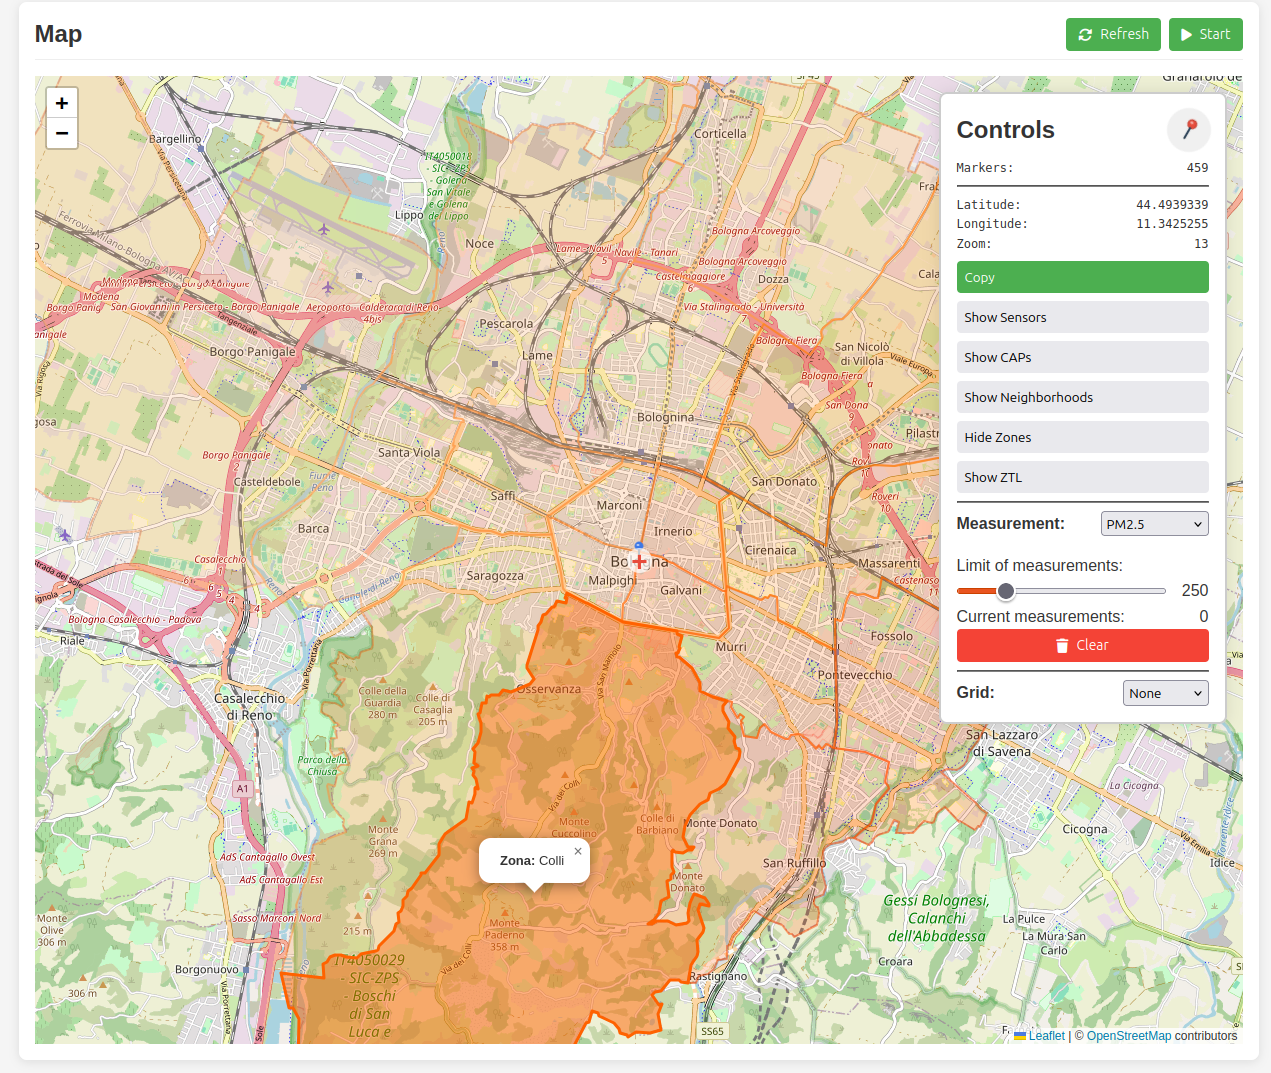
\includegraphics[width=\textwidth]{dashboard/10_map_zones_controls.png}
    \caption{Livello a zone}
    \label{fig:map-layer-zones}
  \end{subfigure}
  \hfill
  \begin{subfigure}{0.48\textwidth}
    \centering
    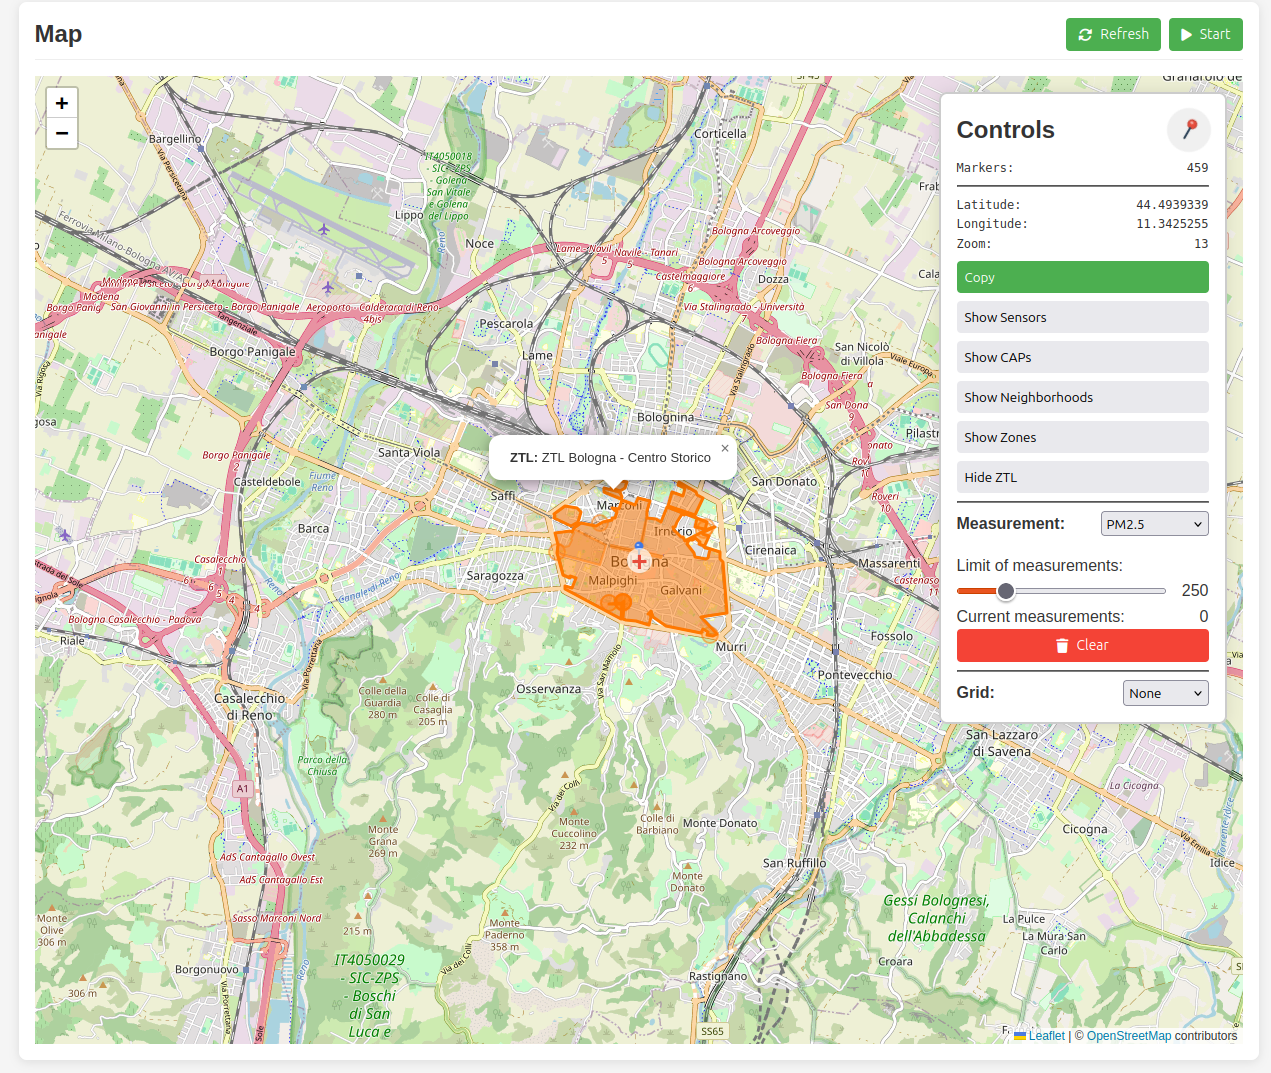
\includegraphics[width=\textwidth]{dashboard/11_map_ztl_controls.png}
    \caption{Livello \acrshort{ztl}}
    \label{fig:map-layer-ztl}
  \end{subfigure}


  \caption{Livelli mappa}
  \label{fig:app-map-levels}
\end{figure}

\newpage

\begin{figure}[H]
  \centering

  \begin{subfigure}{0.48\textwidth}
    \centering
    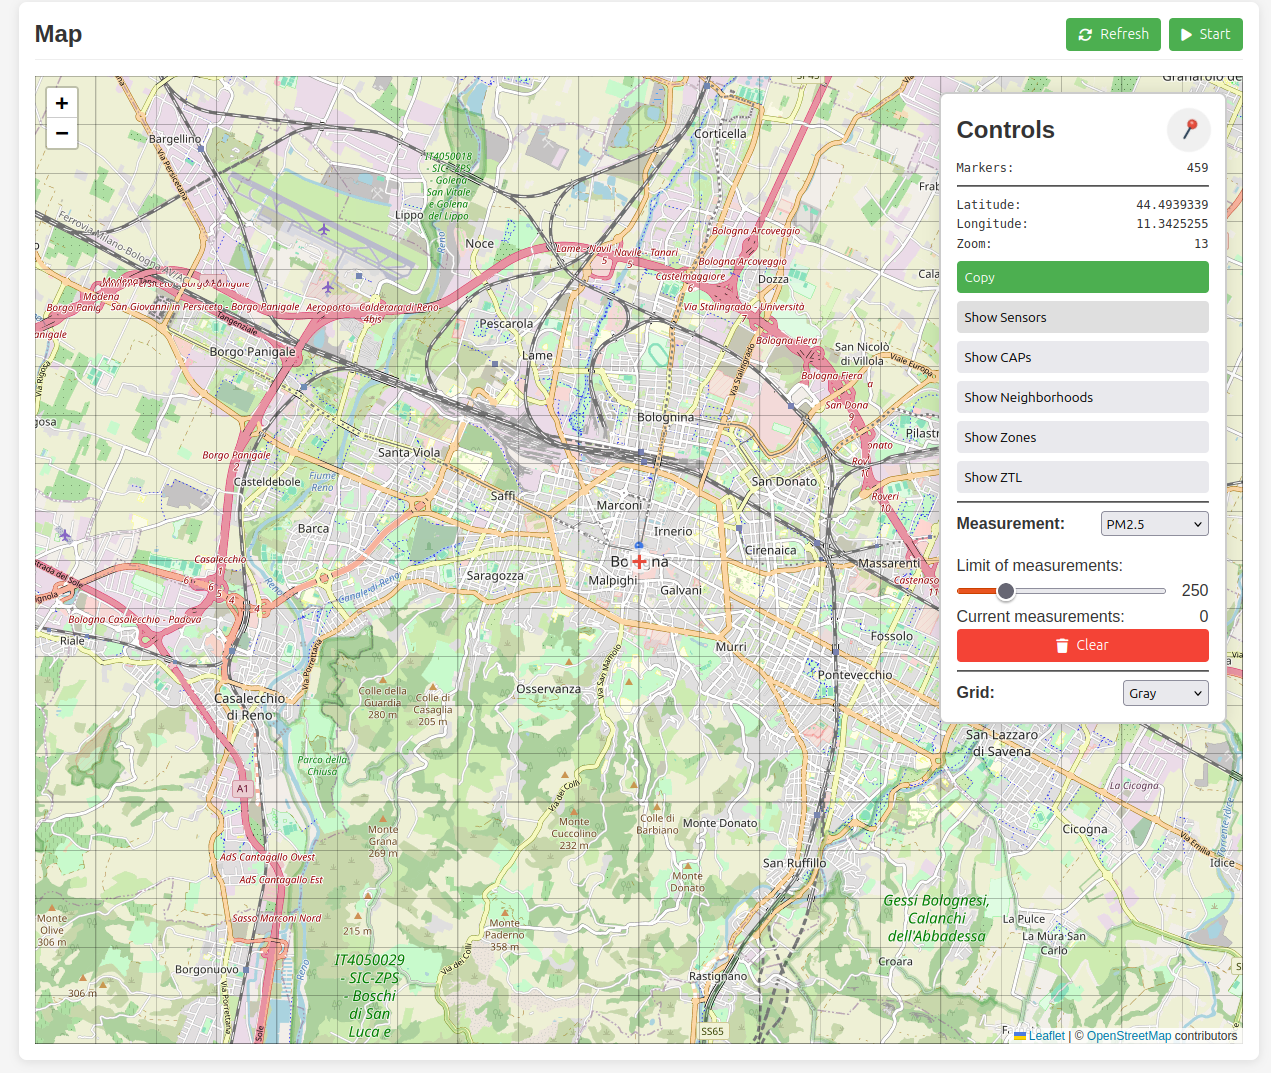
\includegraphics[width=\textwidth]{dashboard/12_map_grid_gray_controls.png}
    \caption{Griglia grigia}
    \label{fig:map-grid-gray}
  \end{subfigure}
  \hfill
  \begin{subfigure}{0.48\textwidth}
    \centering
    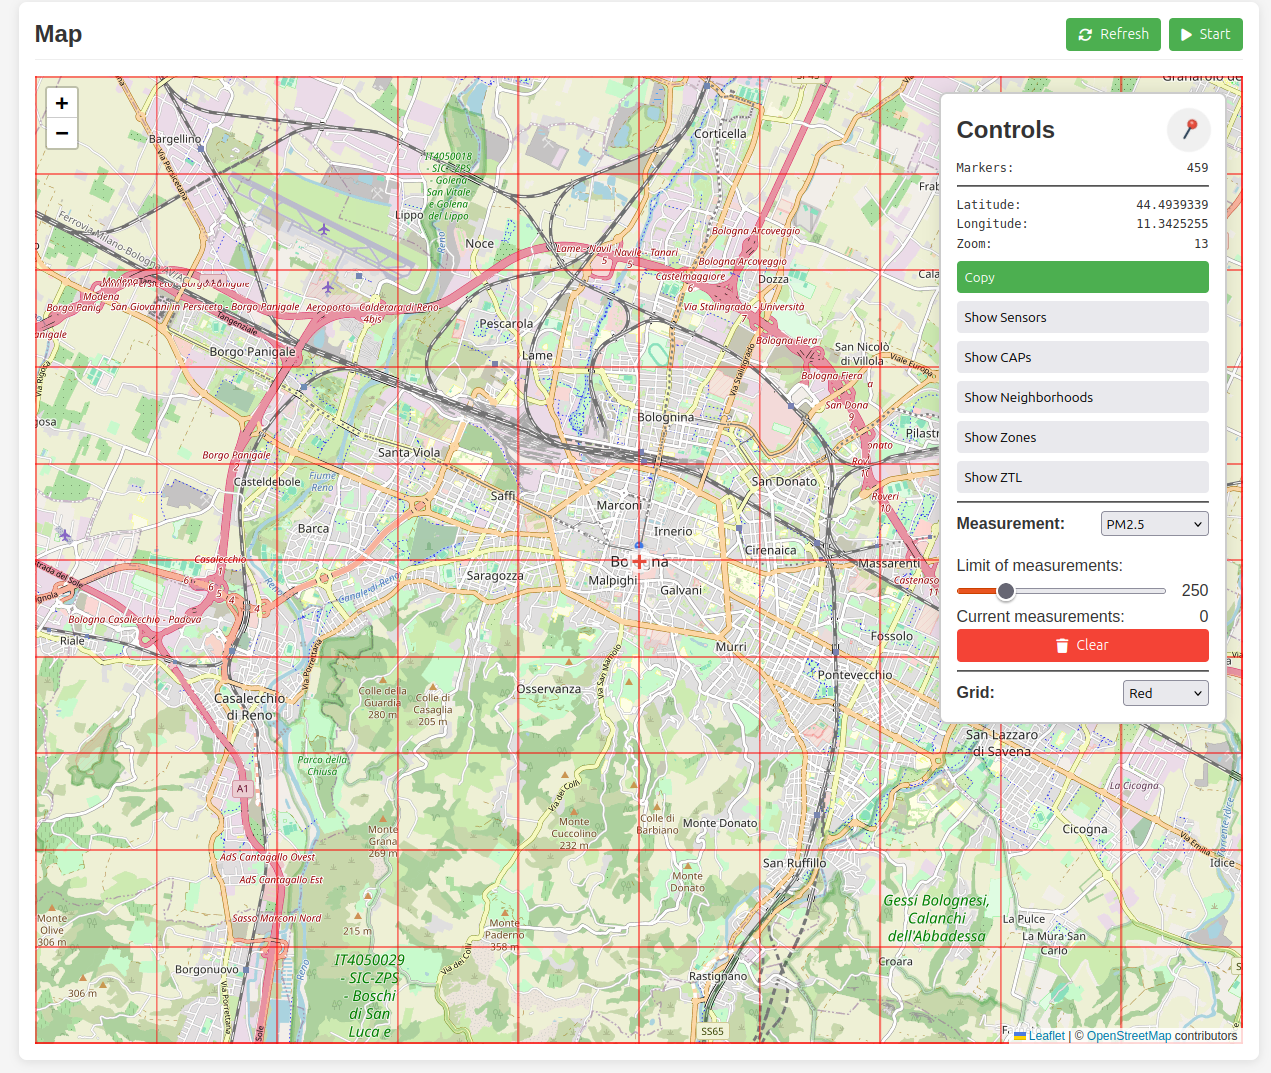
\includegraphics[width=\textwidth]{dashboard/13_map_grid_red_controls.png}
    \caption{Griglia rossa}
    \label{fig:map-grid-red}
  \end{subfigure}

  \vspace{1em}

  \begin{subfigure}{0.48\textwidth}
    \centering
    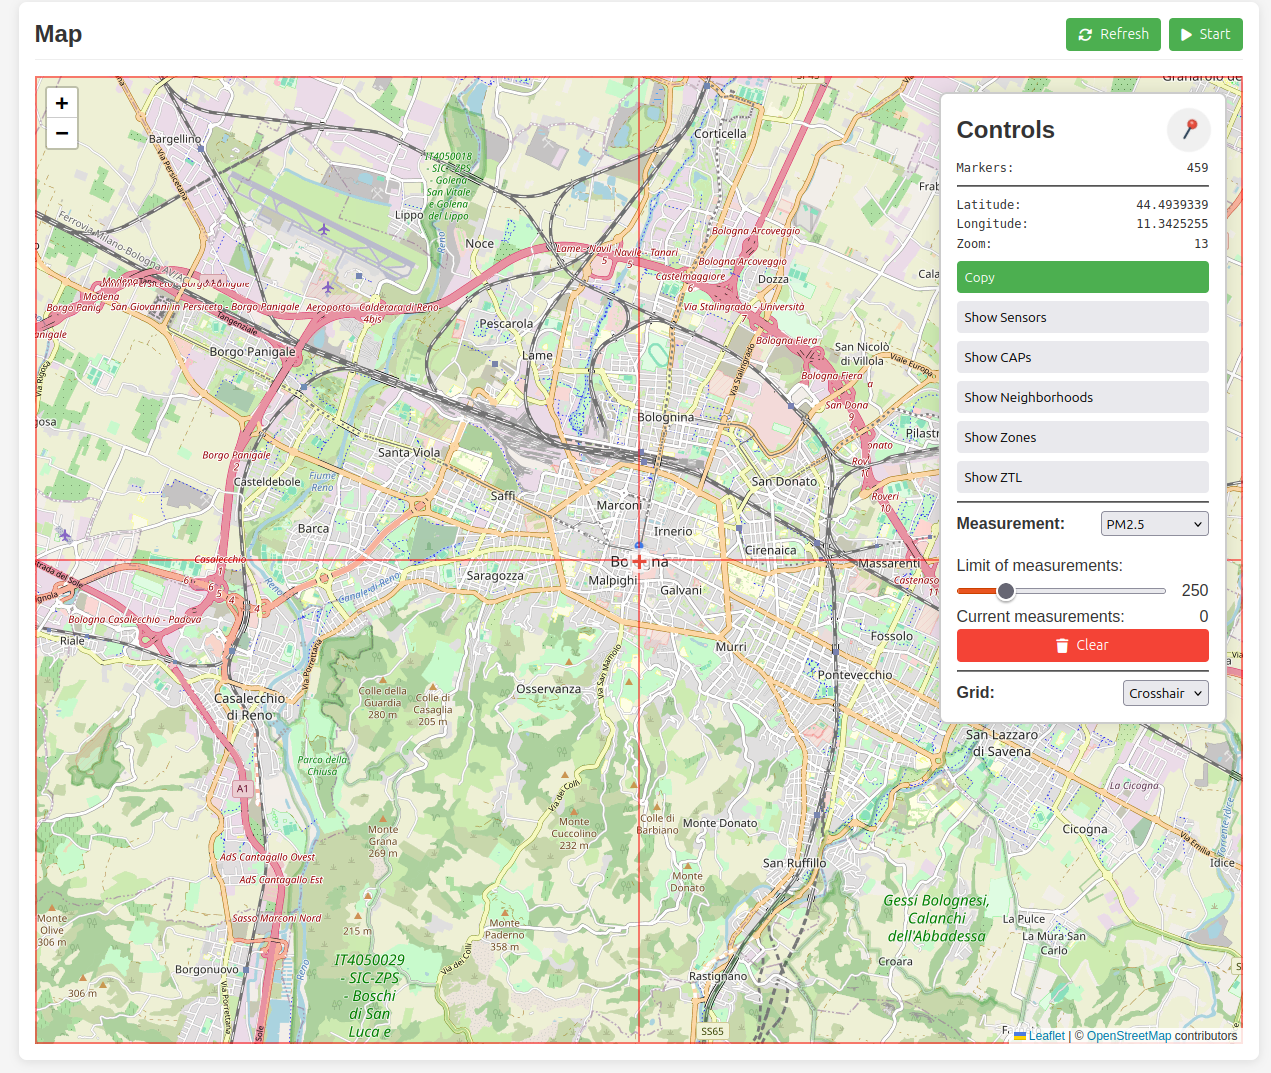
\includegraphics[width=\textwidth]{dashboard/14_map_grid_crosshair_controls.png}
    \caption{Griglia crosshair}
    \label{fig:map-grid-crosshair}
  \end{subfigure}

  \caption{Griglie mappa}
  \label{fig:app-map-grids}
\end{figure}

\newpage

\paragraph{Heatmap}

Una heatmap (mappa di calore) è una rappresentazione grafica bidimensionale di dati in cui i valori individuali,
contenuti in una matrice, sono rappresentati attraverso colori \citep{wilkinson2009grammar}.
Questa tecnica di visualizzazione permette di identificare rapidamente pattern, correlazioni e anomalie
all'interno di dataset complessi mediante l'uso di una scala cromatica che associa intensità di colore
a valori numerici \citep{cleveland1993visualizing}. Il suo utilizzo aiuta a rendere più intuitiva la distribuzione
dei dati poiché a maggior concentrazione risulta un colore più intenso, facilitandone la comprensione ed attirando
l'attenzione sui principali focolai.

Formalmente, data una matrice $M \in \mathbb{R}^{m \times n}$ dove $M_{ij}$ rappresenta il valore
nella posizione $(i,j)$, una heatmap è una funzione di mappatura $ f: M_{ij} \rightarrow C_{ij} $
dove $C_{ij}$ è il colore corrispondente al valore $M_{ij}$ secondo una scala cromatica predefinita.

La scelta della palette di colori è cruciale per l'efficacia comunicativa della heatmap.
È fondamentale utilizzare scale cromatiche che rispettino principi di accessibilità e che siano percettivamente
uniformi \citep{ware2012information}.
Tali colori sono infatti quelli forniti dall'\acrfull{eea} come indicato nella tabella~\ref{tab:air_quality};

Nelle immagini seguenti viene mostrata la heatmap relativa alle misurazioni di \acrshort{pm25}.
Partendo dalla vista default in immagine \ref{fig:app-map-pm25-controls-15},
passiamo ad una versione con zoom inferiore senza sensori (figura~\ref{fig:app-map-pm25-controls-16}) e con sensori
(figura~\ref{fig:app-map-pm25-controls-17}). Successivamente diminuiamo ulteriormente lo zoom senza sensori
(figura~\ref{fig:app-map-pm25-controls-18}), per poi riavvicinarci (figura~\ref{fig:app-map-pm25-controls-19}),
visualizzarle la \acrshort{ztl} (figura~\ref{fig:app-map-pm25-controls-20}) ed i quartieri
(figura~\ref{fig:app-map-pm25-controls-21}). Infine, visualizziamo una versione con concentrazioni più elevate
(figura~\ref{fig:app-map-pm25-controls-22}) rispetto alle prime, essendo passato più tempo ed avendo quindi un numero
maggiore di misurazioni, e le altre misurazioni disponibili (figura~\ref{fig:app-map-pm25-controls-23}).

Come anticipato, allontanarci dal centro della mappa porterà a concentrazioni maggiori, mentre avvicinarci il contrario.
Anche il numero di misurazioni influisce sulle concentrazioni della mappa di calore, essendo direttamente correlate.
% L'utilizzo delle zone delimitate quali ZTL ed i quartieri può essere utile qualora si voglia verificare
% eventuali correlazioni fra le aree di maggiore concentrazione di inquinanti ed i confini amministrativi.

\begin{figure}[H]
  \centering

  \begin{subfigure}{0.48\textwidth}
    \centering
    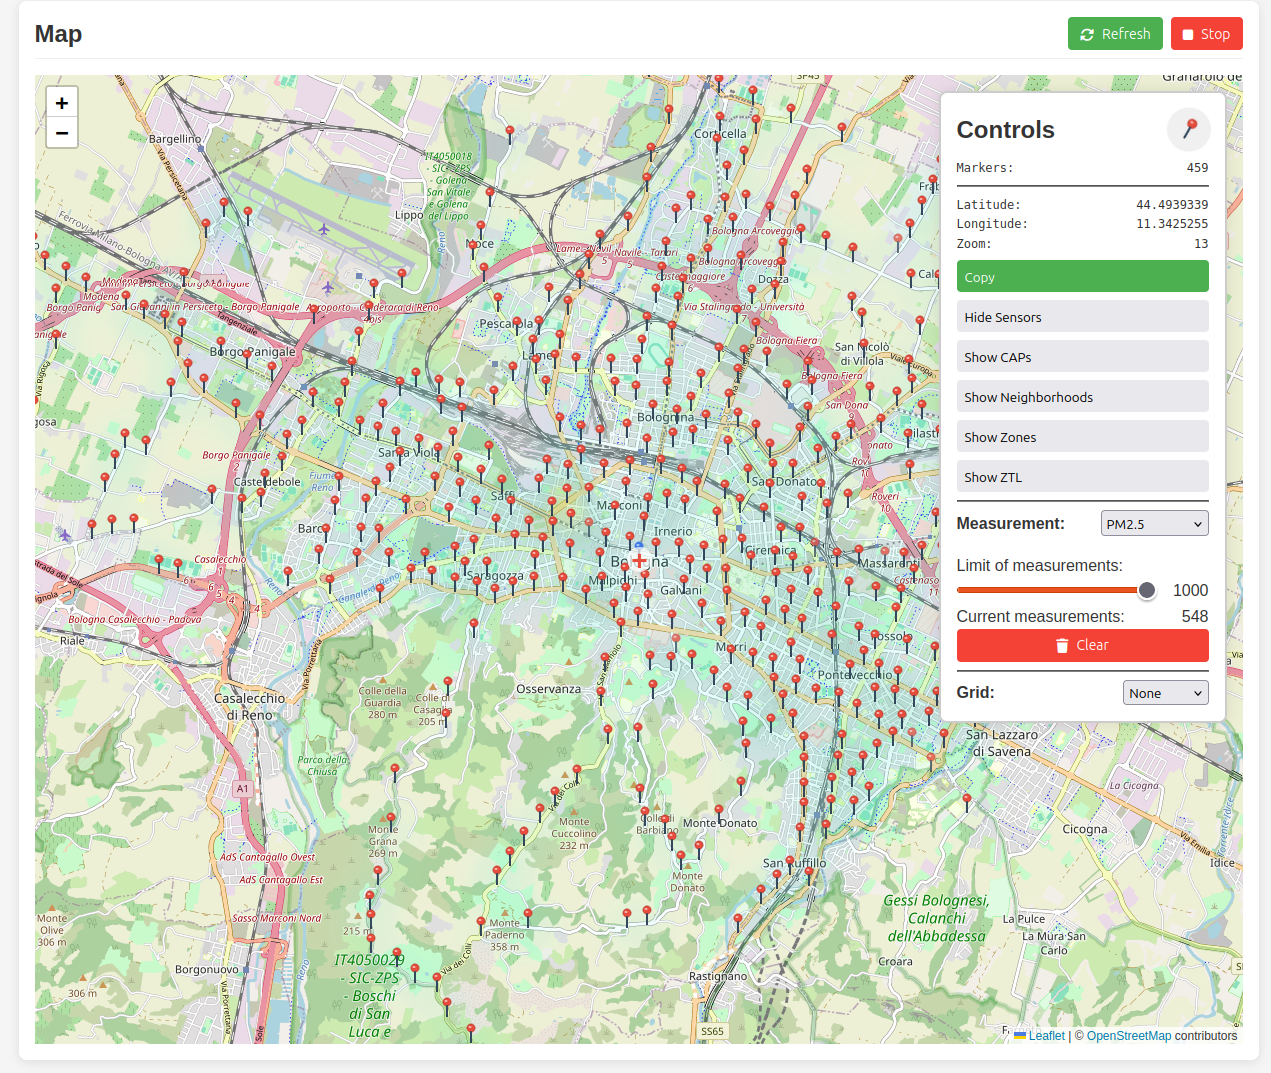
\includegraphics[width=\textwidth]{dashboard/15_map_pm25_controls.png}
    \caption{Heatmap default}
    \label{fig:app-map-pm25-controls-15}
  \end{subfigure}
  \hfill
  \begin{subfigure}{0.48\textwidth}
    \centering
    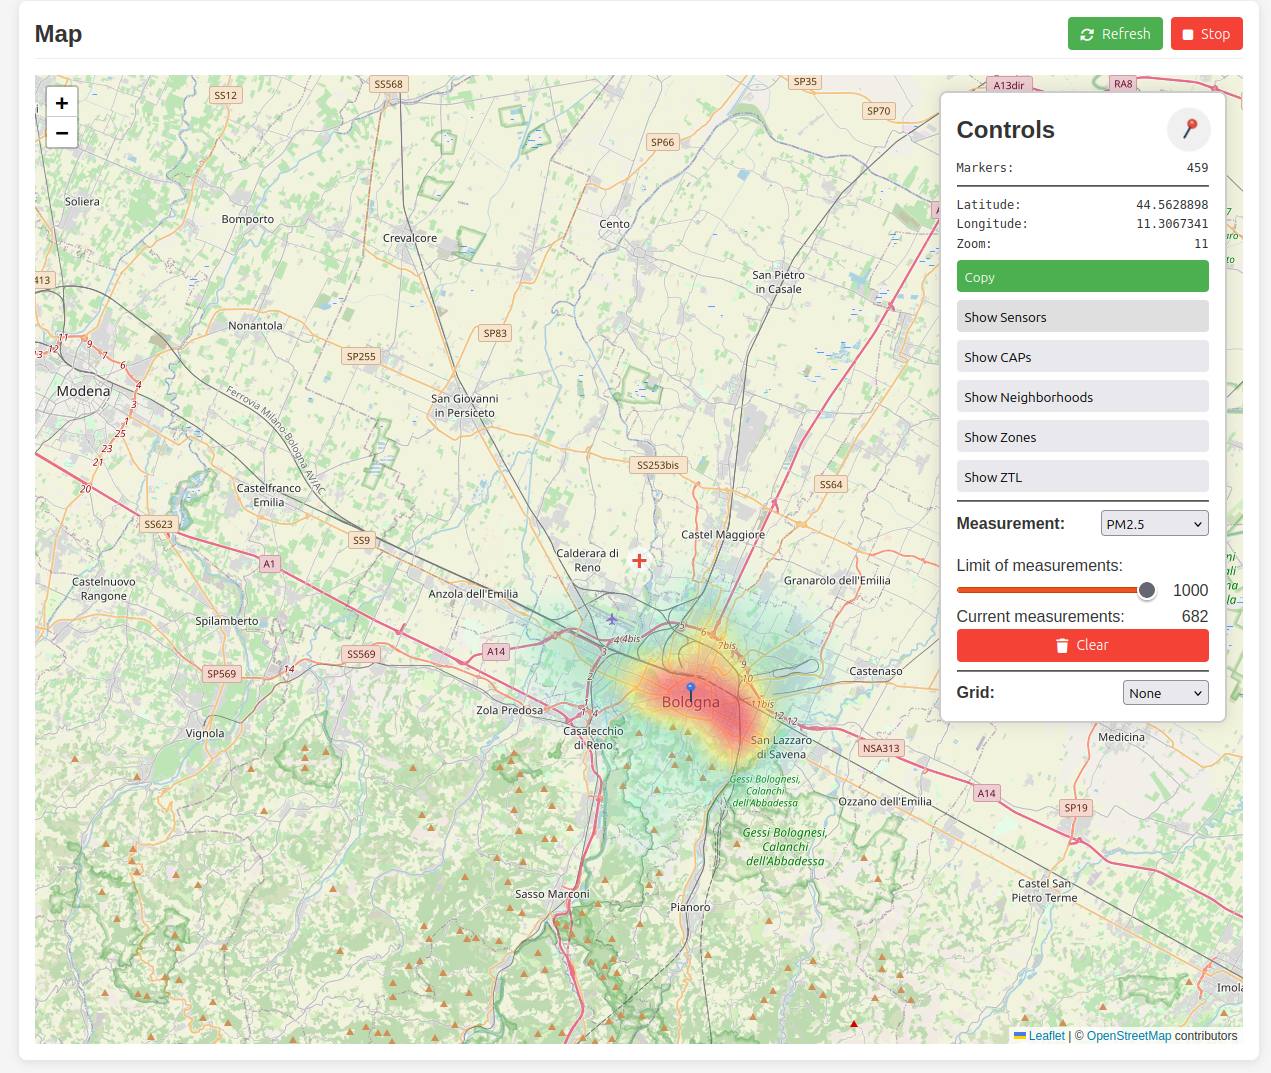
\includegraphics[width=\textwidth]{dashboard/16_map_pm25_controls.png}
    \caption{Heatmap zoom 11 senza sensori}
    \label{fig:app-map-pm25-controls-16}
  \end{subfigure}

  \vspace{1em}

  \begin{subfigure}{0.48\textwidth}
    \centering
    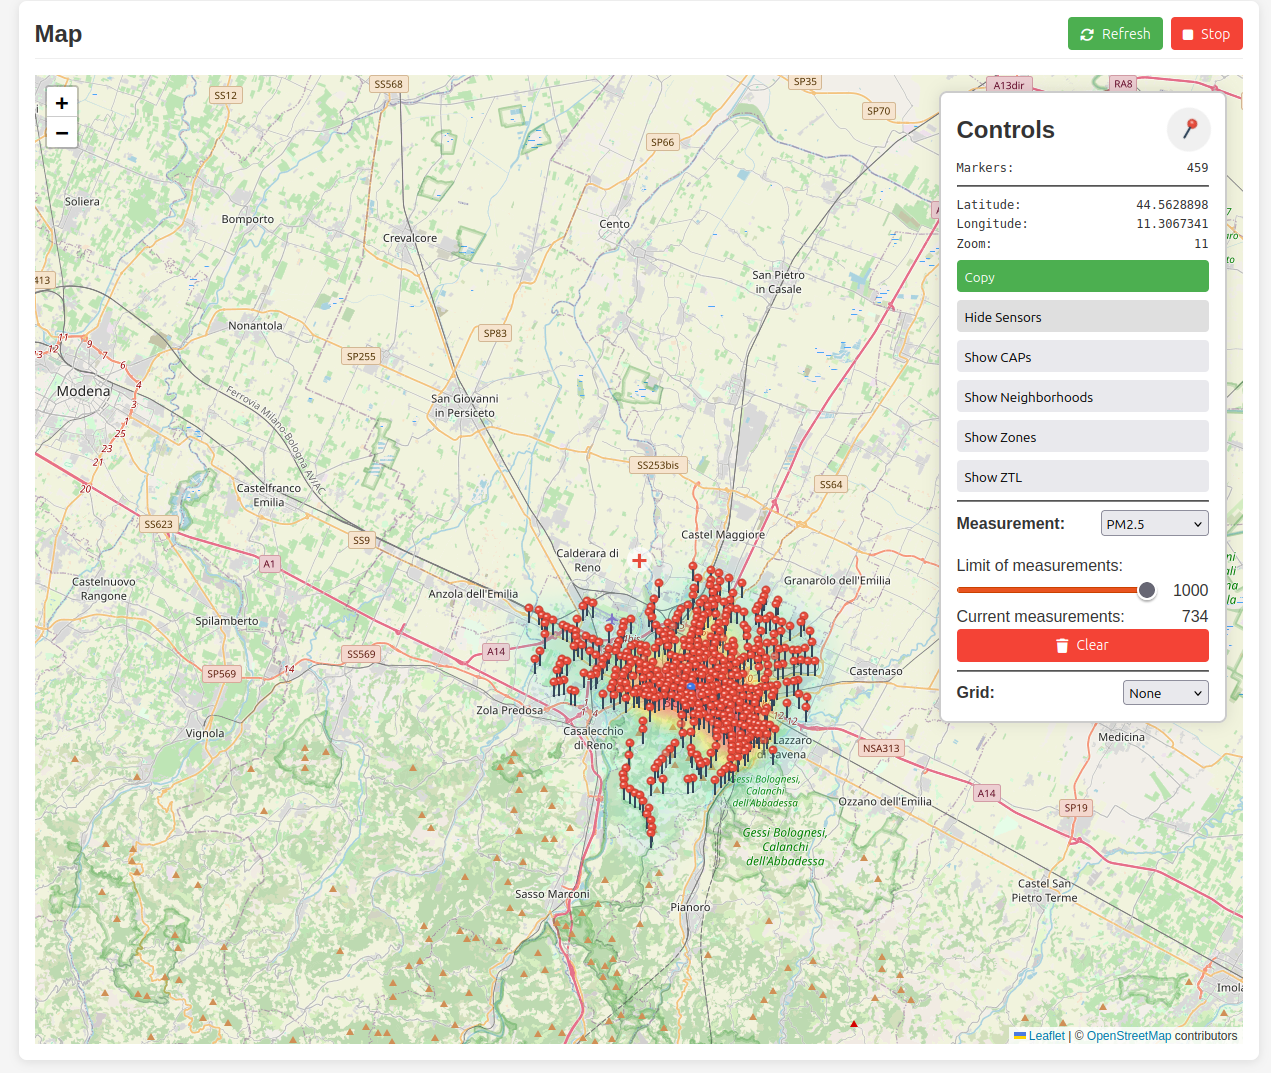
\includegraphics[width=\textwidth]{dashboard/17_map_pm25_controls.png}
    \caption{Heatmap zoom 11 con sensori}
    \label{fig:app-map-pm25-controls-17}
  \end{subfigure}
  \hfill
  \begin{subfigure}{0.48\textwidth}
    \centering
    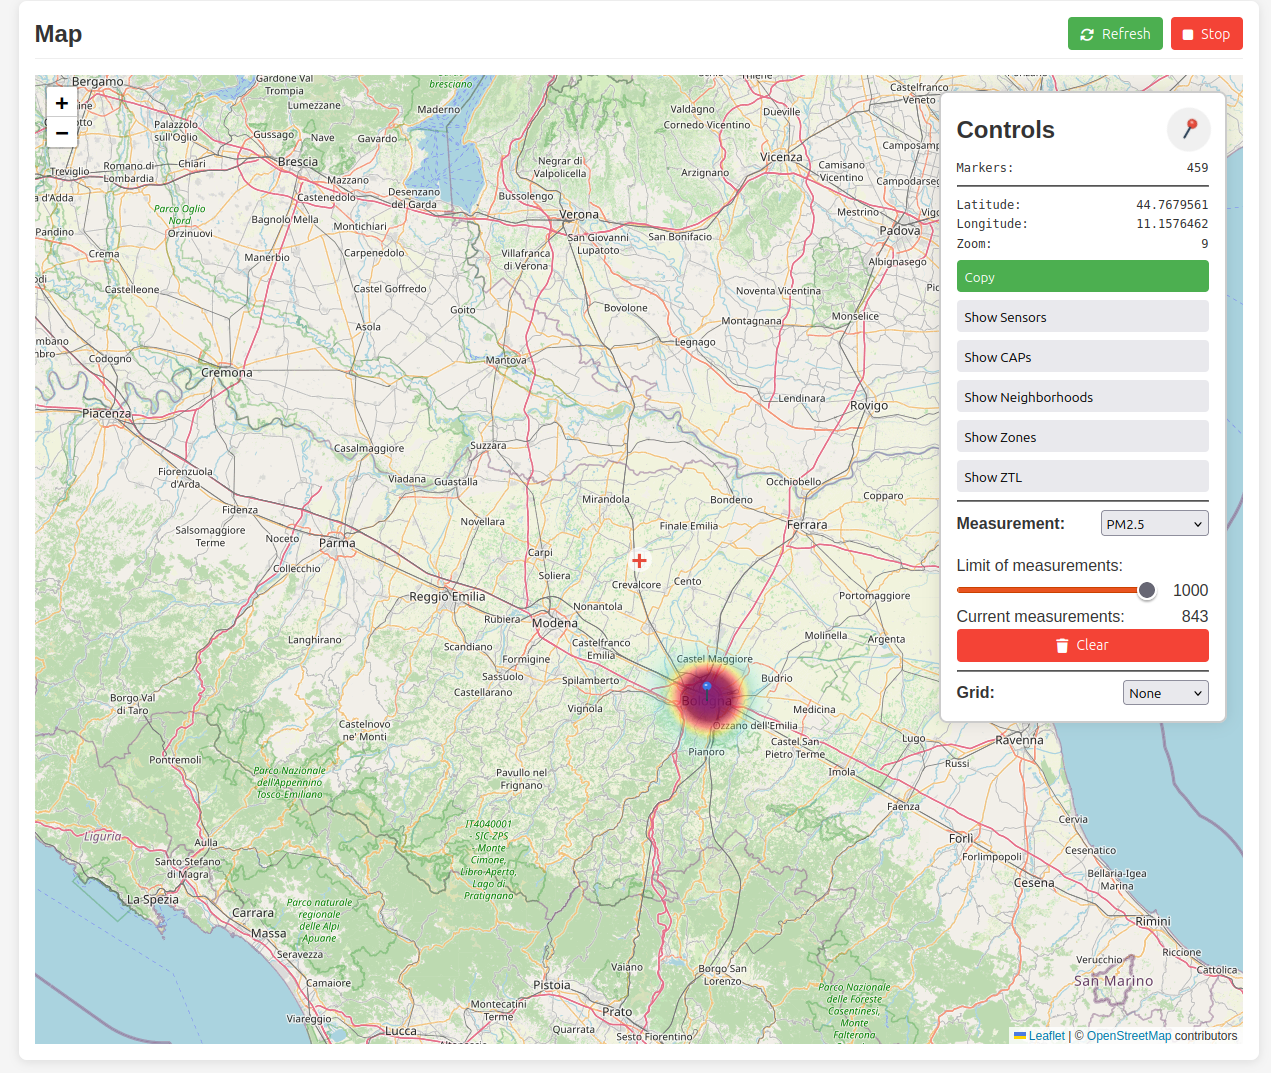
\includegraphics[width=\textwidth]{dashboard/18_map_pm25_controls.png}
    \caption{Heatmap zoom 9 senza sensori}
    \label{fig:app-map-pm25-controls-18}
  \end{subfigure}

  \vspace{1em}

  \begin{subfigure}{0.48\textwidth}
    \centering
    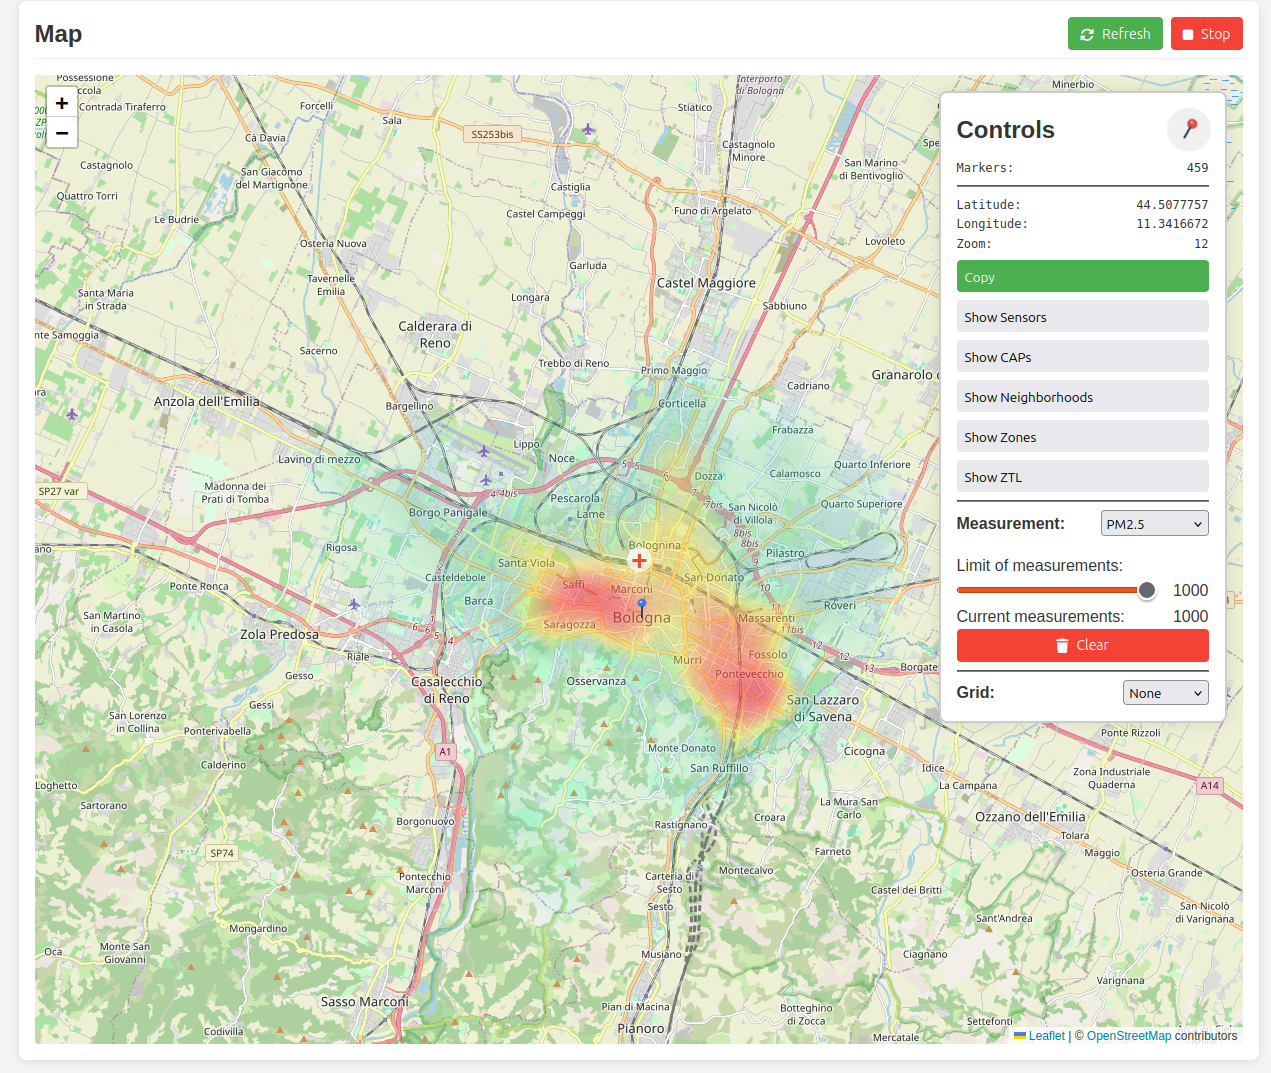
\includegraphics[width=\textwidth]{dashboard/19_map_pm25_controls.png}
    \caption{Heatmap zoom 12 senza sensori}
    \label{fig:app-map-pm25-controls-19}
  \end{subfigure}
  \hfill
  \begin{subfigure}{0.48\textwidth}
    \centering
    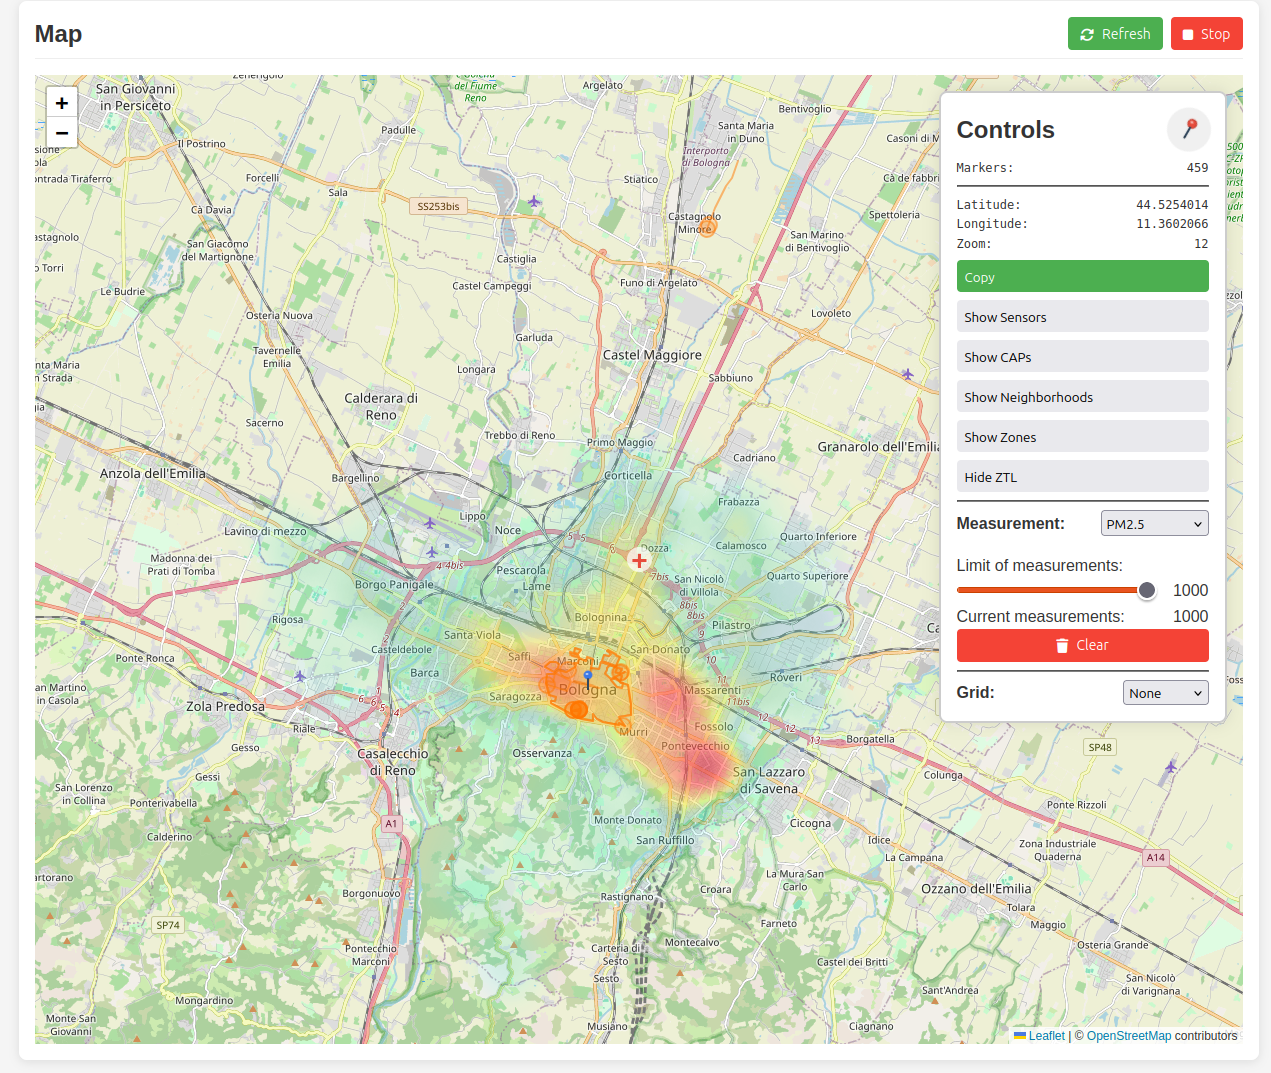
\includegraphics[width=\textwidth]{dashboard/20_map_pm25_controls.png}
    \caption{Heatmap zoom 12 senza sensori \acrshort{ztl}}
    \label{fig:app-map-pm25-controls-20}
  \end{subfigure}

  \caption{Heatmap - parte 1}
  \label{fig:app-map-heatmap-1}
\end{figure}

\begin{figure}[H]
  \centering

  \begin{subfigure}{0.48\textwidth}
    \centering
    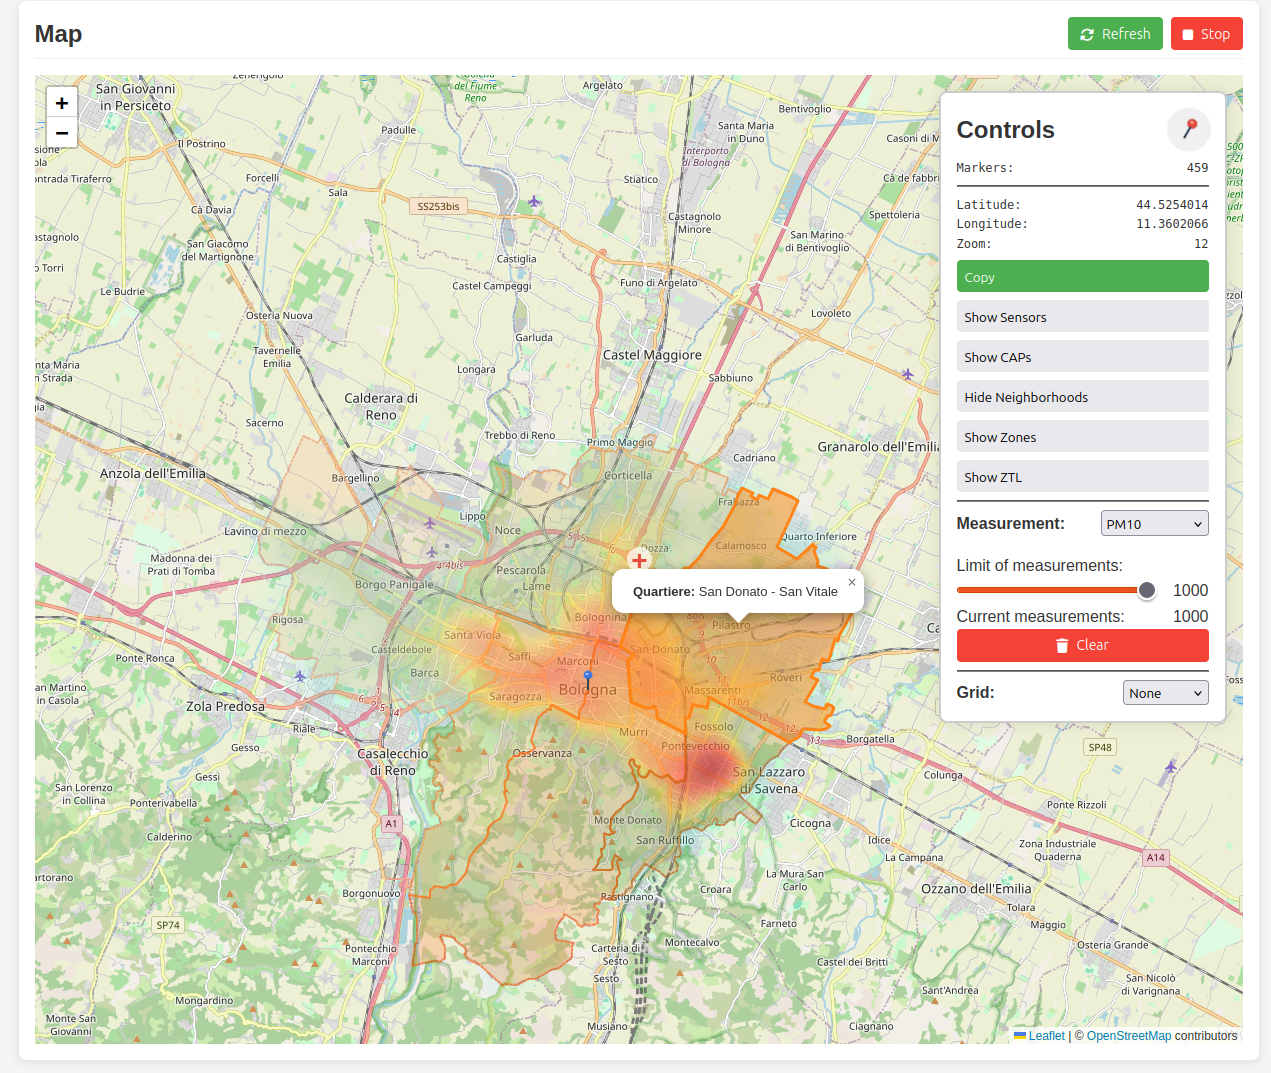
\includegraphics[width=\textwidth]{dashboard/21_map_pm25_controls.png}
    \caption{Heatmap zoom 12 senza sensori con quartieri}
    \label{fig:app-map-pm25-controls-21}
  \end{subfigure}
  \hfill
  \begin{subfigure}{0.48\textwidth}
    \centering
    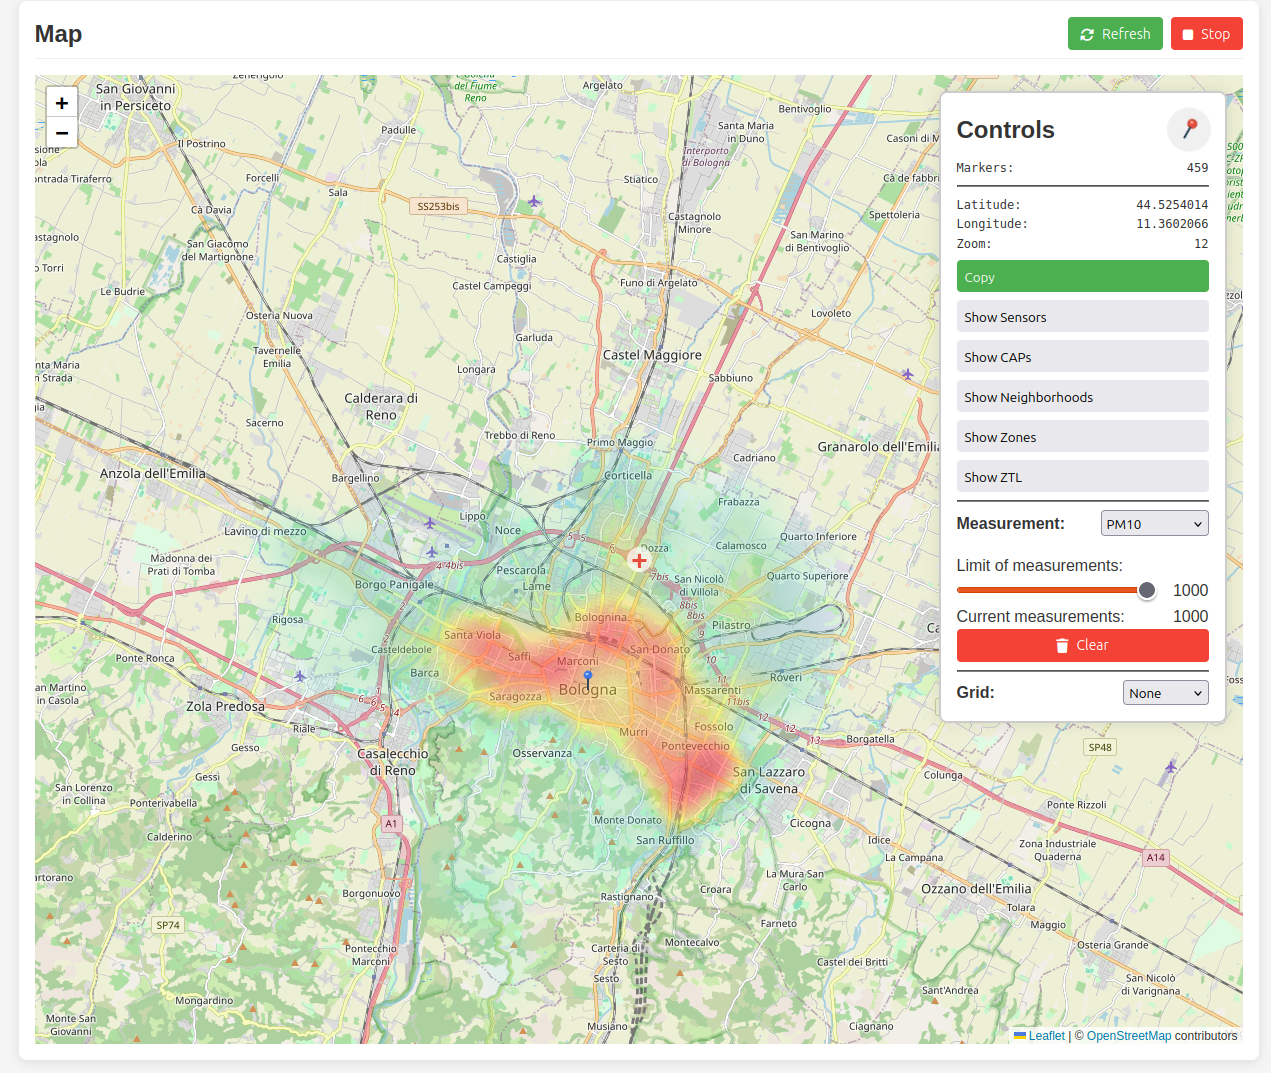
\includegraphics[width=\textwidth]{dashboard/22_map_pm25_controls.png}
    \caption{Heatmap zoom 12 senza sensori, concentrazione maggiore}
    \label{fig:app-map-pm25-controls-22}
  \end{subfigure}

  \vspace{1em}

  \begin{subfigure}{0.48\textwidth}
    \centering
    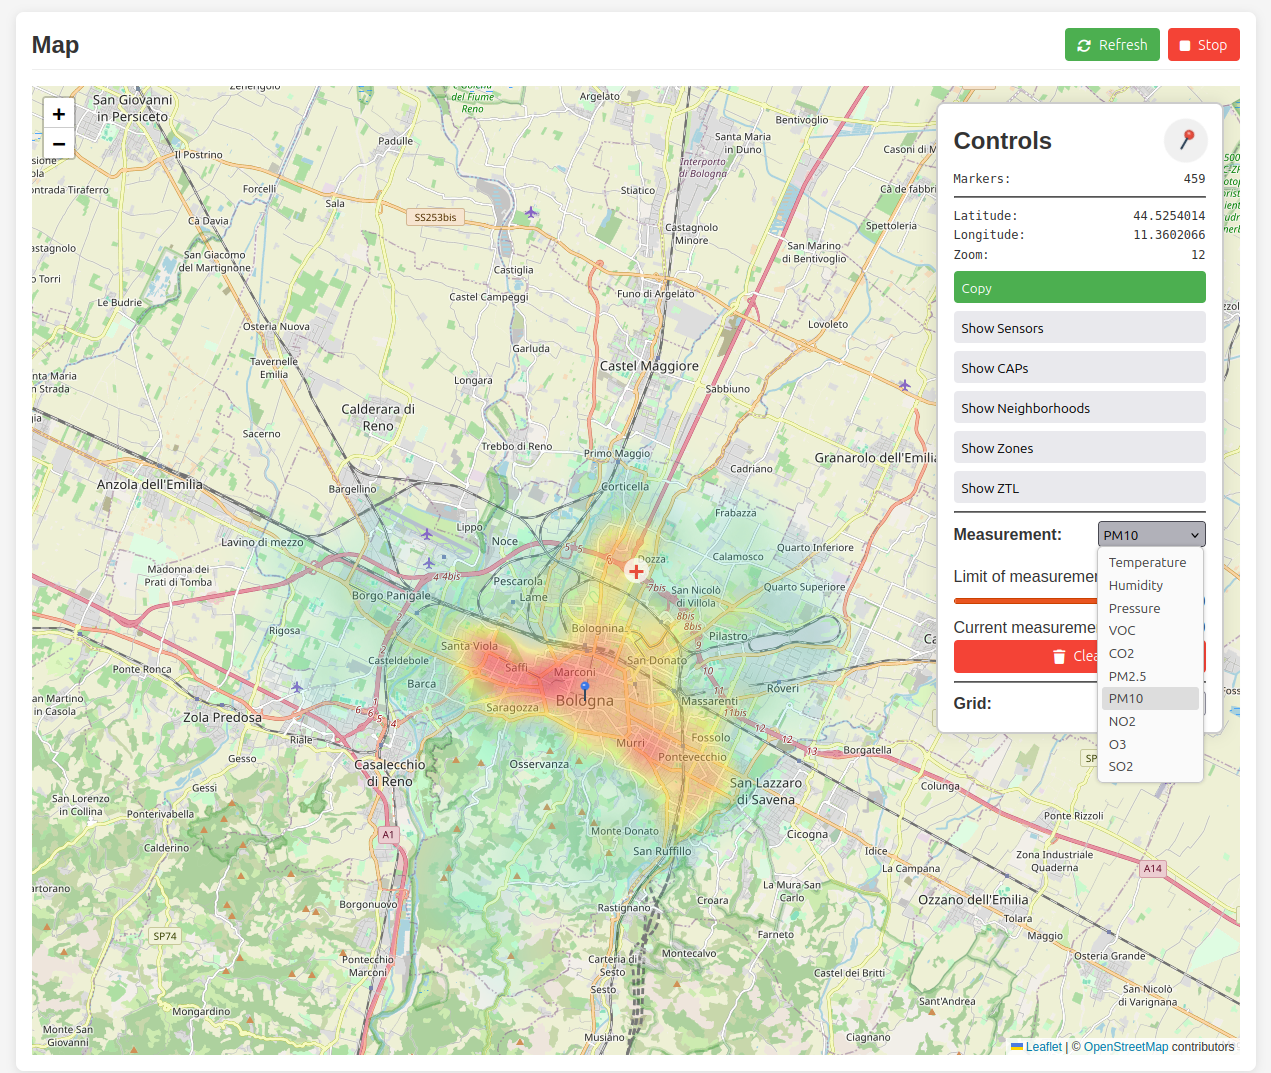
\includegraphics[width=\textwidth]{dashboard/23_map_pm25_controls.png}
    \caption{Heatmap zoom 12 senza sensori, apertura lista misurazioni disponibili}
    \label{fig:app-map-pm25-controls-23}
  \end{subfigure}

  \caption{Heatmap - parte 2}
  \label{fig:app-map-heatmap-2}
\end{figure}

\newpage

\paragraph{Ultime misurazioni}

La tabella delle misurazioni illustrata nella figura~\ref{fig:app-tab-last-measurements} offre una visualizzazione
organizzata delle ultime 50 rilevazioni acquisite dal sistema. Ogni misurazione viene presentata su una riga separata,
contenente informazioni essenziali come l'identificativo del sensore, il momento preciso dell'acquisizione e tutti
i parametri rilevati con le corrispondenti unità di misura.
L'interfaccia è progettata per facilitare la navigazione: selezionando una qualsiasi riga della tabella,
l'utente viene automaticamente reindirizzato alla vista mappa centrata sul sensore responsabile
di quella specifica rilevazione. Questa funzionalità permette di collegare rapidamente i dati numerici alla
loro posizione geografica, offrendo una comprensione più completa delle informazioni raccolte.
La struttura tabulare garantisce una consultazione rapida e ordinata dei dati più recenti,
mantenendo sempre visibili le informazioni più aggiornate del sistema di monitoraggio.

\begin{figure}[H]
  \centering
  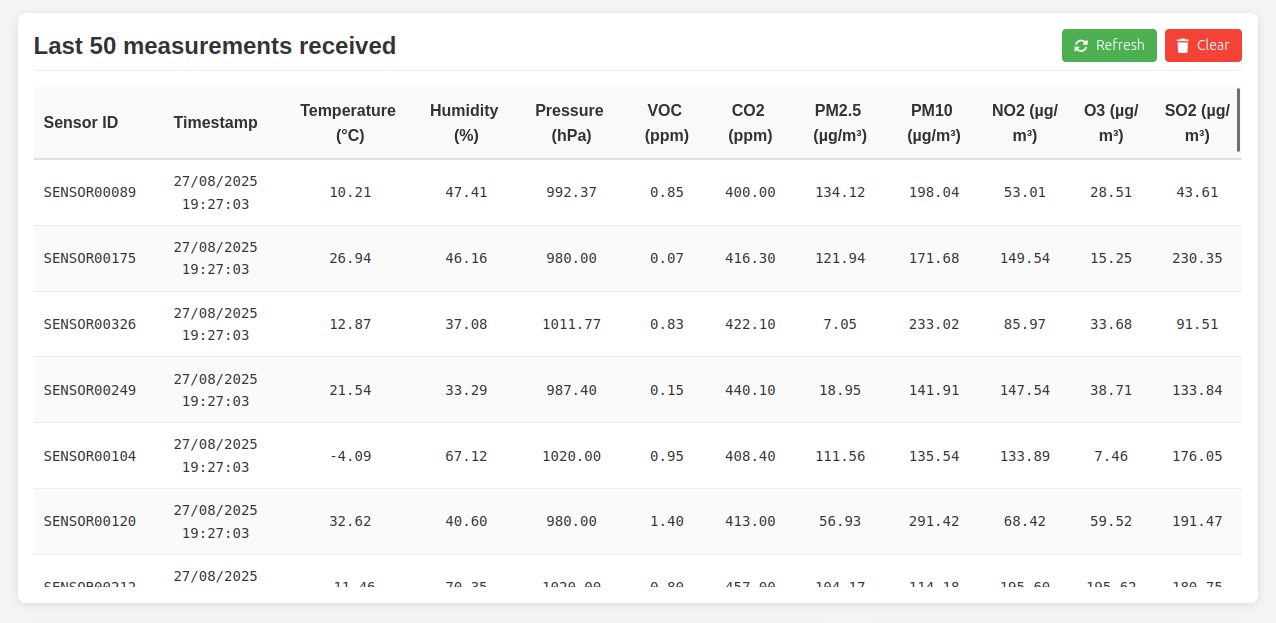
\includegraphics[width=\textwidth]{dashboard/24_table_last_measurements.png}
  \caption{Tabella ultime misurazioni}
  \label{fig:app-tab-last-measurements}
\end{figure}

\newpage

\paragraph{Statistiche}

La tabella delle statistiche riportata nell'immagine~\ref{fig:app-tab-statistics} fornisce un'analisi completa
dei dati per ogni tipologia di misurazione ambientale raccolta dal sistema. Il processo di elaborazione calcola
automaticamente gli indicatori statistici fondamentali: vengono determinati valore medio e mediana
per identificare la tendenza centrale, mentre i valori minimo e massimo evidenziano gli estremi registrati.
Il range di variazione, ottenuto dalla differenza tra questi due estremi, quantifica l'ampiezza
delle oscillazioni rilevate.
Oltre agli indicatori numerici, il sistema integra una valutazione qualitativa dell'aria specifica
per ciascun tipo di inquinante monitorato.
Questa analisi applica criteri di classificazione standardizzati riportati nella tabella~\ref{tab:air_quality},
i quali traducono i valori numerici in categorie comprensibili, accompagnate da un sistema di colori intuitivo
che permette di identificare immediatamente il livello di qualità raggiunto.
L'approccio combinato tra dati statistici e valutazione qualitativa offre agli utenti sia una comprensione
tecnica dettagliata che un'interpretazione immediata dello stato ambientale monitorato.

\begin{figure}[H]
  \centering
  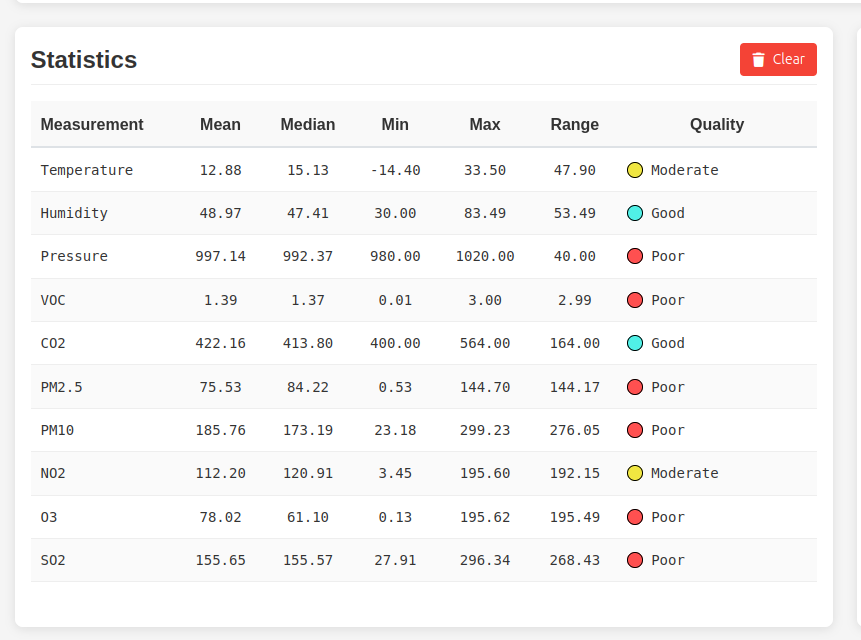
\includegraphics[width=0.9\textwidth]{dashboard/25_table_statistics.png}
  \caption{Tabella statistiche}
  \label{fig:app-tab-statistics}
\end{figure}

\newpage

\paragraph{Log di sistema}

L'applicazione mantiene un registro completo delle attività utente attraverso una tabella di log che documenta tutte
le interazioni, sia quelle effettuate tramite interfaccia grafica che attraverso chiamate \acrshort{api}, come si
può vedere nell'immagine~\ref{fig:app-tab-system-log}.
Il sistema traccia diversi tipi di eventi: l'arrivo di nuove misurazioni dai sensori, i clic sui dispositivi
nell'interfaccia, le operazioni di registrazione dei sensori e l'attivazione o disattivazione della ricezione dati.
Per ottimizzare la visualizzazione, il log raggruppa automaticamente gli eventi identici che si verificano
nel medesimo secondo, mostrando il numero di occorrenze (in grigio) accanto alla voce principale.
Questa funzionalità evita la duplicazione di informazioni e mantiene il registro più leggibile.
Il sistema limita la visualizzazione a un massimo di 25 righe per garantire prestazioni ottimali e una consultazione
agevole. Quando questo limite viene raggiunto, le voci più recenti sostituiscono automaticamente quelle più datate,
assicurando che il log mostri sempre le attività più attuali del sistema.

\begin{figure}[H]
  \centering
  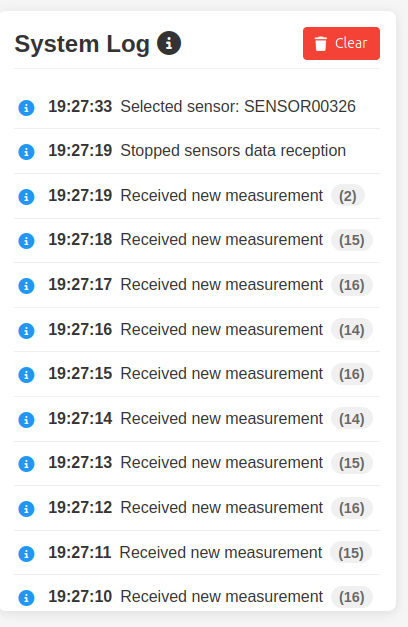
\includegraphics[width=0.45\textwidth]{dashboard/26_table_system_log.png}
  \caption{Tabella log di sistema}
  \label{fig:app-tab-system-log}
\end{figure}

\newpage

\paragraph{Tabella dei sensori registrati}

La parte finale della pagina principale riporta la tabella dei sensori registrati.

Questa tabella è formata da diverse colonne, quali l'id del sensore, latitudine, longitudine, stato,
distanza dal centro della mappa, data ultima misurazione registrata e relativo tempo trascorso da essa.

\begin{figure}[H]
  \centering
  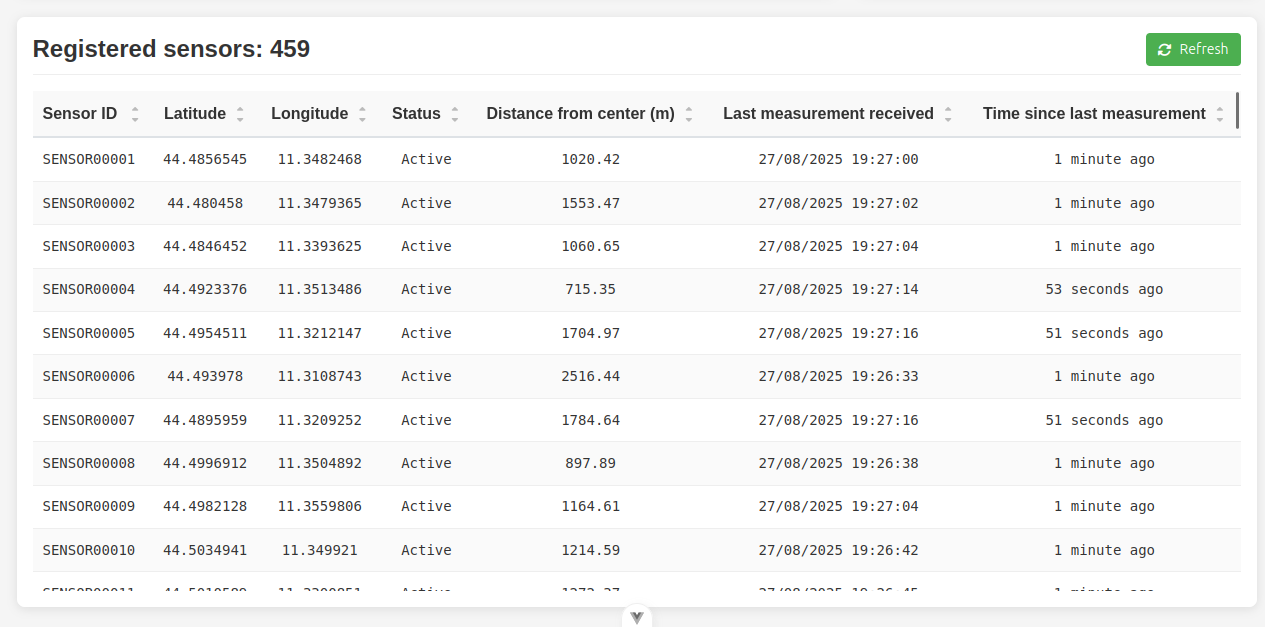
\includegraphics[width=\textwidth]{dashboard/27_table_registered_sensors.png}
  \caption{Tabella sensori registrati}
  \label{fig:app-tab-registered-sensors}
\end{figure}

% Nella prima immagine~\ref{fig:app-tab-registered-sensors} abbiamo i sensori ordinati per id crescente (default),
% mentre nella seconda~\ref{fig:app-tab-registered-sensors-distance-sort-asc} e
% terza immagine~\ref{fig:app-tab-registered-sensors-distance-sort-desc} si ha la tabella ordinata rispetto
% la distanza dal centro della mappa relativamente in ordine crescente (dal sensore più prossimo al più remoto) e
% decrescente (dal sensore più lontano al più vicino).
% Anche qui, cliccando sulla riga dedicata, la pagina scorre verso la mappa centrata sul sensore indicato.

% \begin{figure}[H]
%   \centering
%   \begin{subfigure}{\textwidth}
%     \centering
%     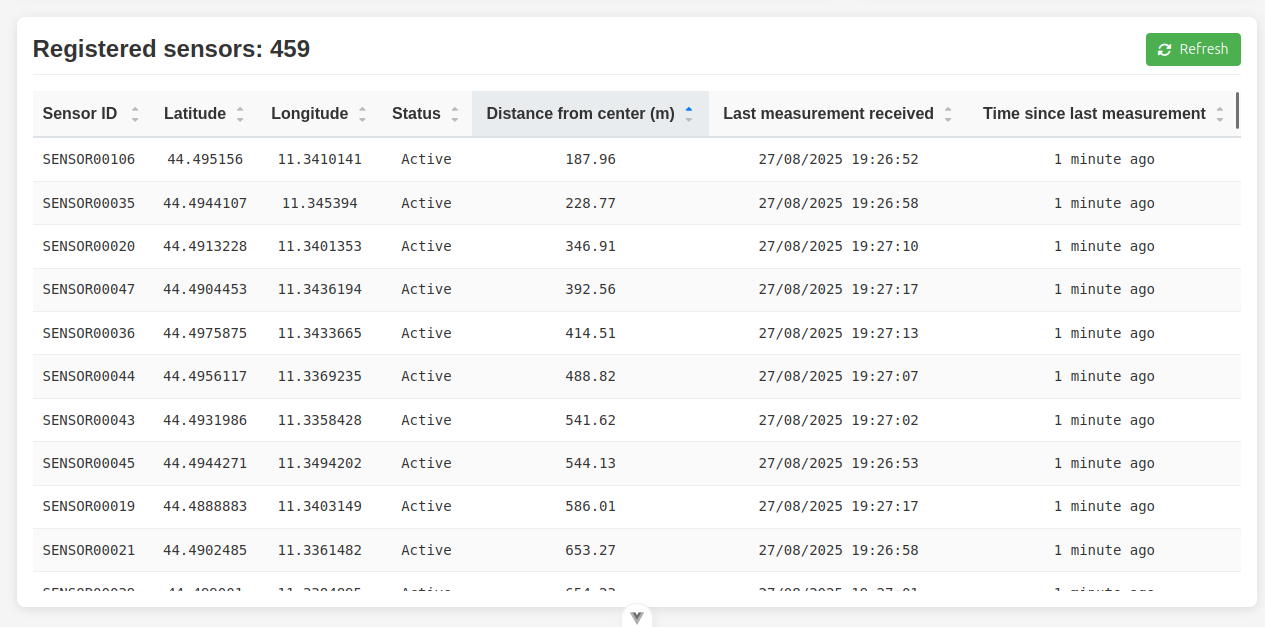
\includegraphics[width=\textwidth]{dashboard/28_table_registered_sensors_distance_sort_asc.png}
%     \caption{Tabella sensori registrati, ordinati per "distanza dal centro" crescente}
%     \label{fig:app-tab-registered-sensors-distance-sort-asc}
%   \end{subfigure}

%   \hfill
%   \begin{subfigure}{\textwidth}
%     \centering
%     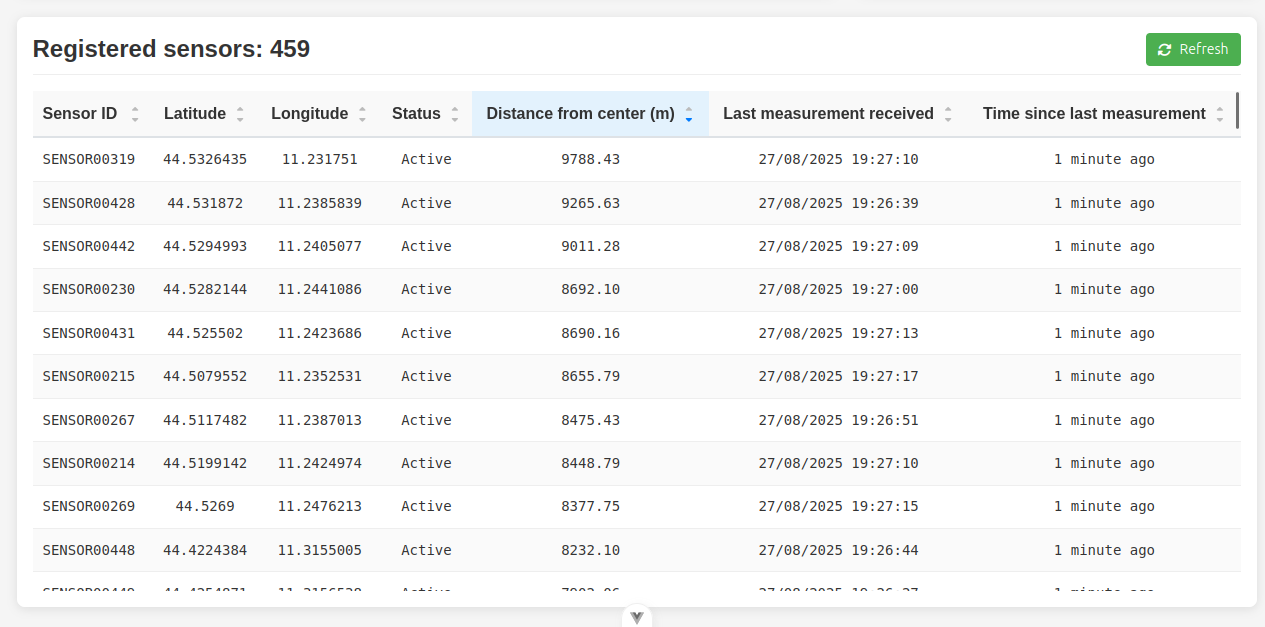
\includegraphics[width=\textwidth]{dashboard/29_table_registered_sensors_distance_sort_desc.png}
%     \caption{Tabella sensori registrati, ordinati per "distanza dal centro" decrescente}
%     \label{fig:app-tab-registered-sensors-distance-sort-desc}
%   \end{subfigure}
% \end{figure}

Il calcolo per ottenere la distanza di un sensore dal centro della mappa è realizzato attraverso
la formula di Haversine \cite{haversine_formula}, ovvero una funzione usata per calcolare la distanza ortodromica
(linea retta sulla superficie terrestre) tra due punti. Essendo i sensori dotati di coordinate spaziali
quali latitudine e longitudine, come il centro della mappa, la formula è risultata l'ideale per calcolarne la distanza.

\paragraph{Formula di Haversine}

Di seguito la formula in termini matematici~\ref{lst:haversine-formula-math},
con relativa legenda~\ref{lst:haversine-formula-math-legend}, e la versione
di codice Javascript~\ref{lst:haversine-formula-code} realmente utilizzata dall'applicazione.

\begin{figure}[h]
  \begin{align}
    a & = \sin^2\left(\frac{\Delta\varphi}{2}\right) + \cos\varphi_1 \cdot \cos\varphi_2 \cdot \sin^2\left(\frac{\Delta\lambda}{2}\right) \\
    c & = 2 \cdot \text{atan2}\left(\sqrt{a}, \sqrt{1-a}\right)                                                                           \\
    d & = R \cdot c
  \end{align}
  \caption{Formula matematica di Haversine}
  \label{lst:haversine-formula-math}
\end{figure}

\begin{tabular}{ll}
  \textbf{Simbolo}       & \textbf{Significato}                                \\
  \hline
  $\varphi$              & latitudine (in radianti)                            \\
  $\varphi_1, \varphi_2$ & latitudine del punto 1 e punto 2                    \\
  $\Delta\varphi$        & differenza di latitudine ($\varphi_2 - \varphi_1$)  \\
  $\lambda$              & longitudine (in radianti)                           \\
  $\lambda_1, \lambda_2$ & longitudine del punto 1 e punto 2                   \\
  $\Delta\lambda$        & differenza di longitudine ($\lambda_2 - \lambda_1$) \\
  $R$                    & raggio terrestre medio ($\sim 6371$ km)             \\
  $d$                    & distanza tra i punti (in metri o km)                \\
  $c$                    & distanza angolare (in radianti)                     \\
  $a$                    & termine intermedio                                  \\
  \label{lst:haversine-formula-math-legend}
\end{tabular}

\begin{lstlisting}[caption={Formual di Haversine in codice Javascript}, label=lst:haversine-formula-code]
  // Function to calculate the distance between two geographic points (Haversine formula)
  calculateDistance(lat1, lon1, lat2, lon2) {
    const R = 6371000; // Earth radius in meters
    const dLat = ((lat2 - lat1) * Math.PI) / 180;
    const dLon = ((lon2 - lon1) * Math.PI) / 180;
    const a =
      Math.sin(dLat / 2) * Math.sin(dLat / 2) +
      Math.cos((lat1 * Math.PI) / 180) *
      Math.cos((lat2 * Math.PI) / 180) *
      Math.sin(dLon / 2) *
      Math.sin(dLon / 2);
    const c = 2 * Math.atan2(Math.sqrt(a), Math.sqrt(1 - a));
    return R * c;
  }
\end{lstlisting}


%%%%%%%%%%%%%%%%%%%%%%%%%%%%%%%%%%%%%%%%%%%%%%%%%%%%%%%%%%%%%%%%%%%
% Document final section start                                    %
%                                                                 %
% Any appendices, required bibliography,                          %
% Optional table and figure lists (if needed, uncomment           %
% The line containing \listoffigures and \listoftables commands)  %
%%%%%%%%%%%%%%%%%%%%%%%%%%%%%%%%%%%%%%%%%%%%%%%%%%%%%%%%%%%%%%%%%%%

%%%%%%%%%%%%%%%%%%%%%%%%%%%%%%%%%%%%%%%%%non numera l'ultima pagina sinistra
\clearpage{\pagestyle{empty}\cleardoublepage}
%%%%%%%%%%%%%%%%%%%%%%%%%%%%%%%%%%%%%%%%%per fare le conclusioni
\chapter*{Conclusioni}
%%%%%%%%%%%%%%%%%%%%%%%%%%%%%%%%%%%%%%%%%imposta l'intestazione di pagina
\rhead[\fancyplain{}{\bfseries
CONCLUSIONI}]{\fancyplain{}{\bfseries\thepage}}
\lhead[\fancyplain{}{\bfseries\thepage}]{\fancyplain{}{\bfseries
CONCLUSIONI}}
%%%%%%%%%%%%%%%%%%%%%%%%%%%%%%%%%%%%%%%%%aggiunge la voce Conclusioni
                                        %   nell'indice
\addcontentsline{toc}{chapter}{Conclusioni} Queste sono le
conclusioni.\\

Lorem ipsum dolor sit amet, consectetur adipiscing elit. Quisque a magna quis nunc venenatis vestibulum. Curabitur commodo efficitur ipsum, non ullamcorper tellus. Duis dictum commodo nisi nec venenatis. Donec euismod pulvinar finibus. Suspendisse lorem mi, suscipit quis faucibus ut, luctus in justo. Cras pulvinar arcu ut ullamcorper pulvinar. Aliquam dictum tortor quis diam luctus, quis tristique tortor ultrices. Integer et lacus a velit efficitur convallis. Morbi enim erat, fermentum vel nulla id, viverra vehicula nisi. Integer non auctor leo, eu convallis massa. Cras eu cursus ligula. Nunc non purus et sem vehicula viverra ut nec nibh.

Quisque posuere purus quis eros auctor efficitur. Etiam mattis vitae nulla et blandit. Nulla a orci magna. Cras ac elit enim. Vestibulum nec nisl metus. Mauris congue velit nec malesuada scelerisque. Sed dignissim, enim vitae semper fermentum, mauris leo vestibulum nisl, in malesuada nibh felis nec dui.

Nullam sit amet tellus eget mi varius commodo. Vestibulum sit amet egestas odio. Nam in ullamcorper quam, nec efficitur augue. Curabitur eget elit in leo eleifend tempor vel lobortis lorem. Duis neque dui, tempus eu sollicitudin ac, lobortis sit amet odio. Morbi eleifend, tellus a varius consequat, enim erat sagittis justo, ac rutrum ipsum augue in leo. Suspendisse non mi ante.

Praesent sed pretium dui, id volutpat tortor. Suspendisse tortor lorem, vestibulum vitae ullamcorper vitae, tincidunt nec leo. Proin interdum congue blandit. Ut bibendum sagittis leo, nec venenatis urna mollis id. Donec nec erat non justo maximus venenatis. In mollis elit eu odio maximus porta. Vestibulum varius turpis sit amet orci blandit, vitae volutpat erat viverra.

Suspendisse nunc urna, elementum ut purus a, sagittis porta velit. Integer ultricies convallis tortor id pellentesque. Duis et sem a mi bibendum congue. Morbi ut tellus cursus, laoreet ipsum rutrum, condimentum felis. Proin velit mi, ultricies a urna nec, facilisis pretium mi. Pellentesque tristique interdum purus, a facilisis mi tempor quis. Sed finibus venenatis ligula porttitor porttitor. Suspendisse cursus lorem nec velit commodo fringilla.
Lorem ipsum dolor sit amet, consectetur adipiscing elit. Quisque a magna quis nunc venenatis vestibulum. Curabitur commodo efficitur ipsum, non ullamcorper tellus. Duis dictum commodo nisi nec venenatis. Donec euismod pulvinar finibus. Suspendisse lorem mi, suscipit quis faucibus ut, luctus in justo. Cras pulvinar arcu ut ullamcorper pulvinar. Aliquam dictum tortor quis diam luctus, quis tristique tortor ultrices. Integer et lacus a velit efficitur convallis. Morbi enim erat, fermentum vel nulla id, viverra vehicula nisi. Integer non auctor leo, eu convallis massa. Cras eu cursus ligula. Nunc non purus et sem vehicula viverra ut nec nibh.

Quisque posuere purus quis eros auctor efficitur. Etiam mattis vitae nulla et blandit. Nulla a orci magna. Cras ac elit enim. Vestibulum nec nisl metus. Mauris congue velit nec malesuada scelerisque. Sed dignissim, enim vitae semper fermentum, mauris leo vestibulum nisl, in malesuada nibh felis nec dui.

Nullam sit amet tellus eget mi varius commodo. Vestibulum sit amet egestas odio. Nam in ullamcorper quam, nec efficitur augue. Curabitur eget elit in leo eleifend tempor vel lobortis lorem. Duis neque dui, tempus eu sollicitudin ac, lobortis sit amet odio. Morbi eleifend, tellus a varius consequat, enim erat sagittis justo, ac rutrum ipsum augue in leo. Suspendisse non mi ante.

Praesent sed pretium dui, id volutpat tortor. Suspendisse tortor lorem, vestibulum vitae ullamcorper vitae, tincidunt nec leo. Proin interdum congue blandit. Ut bibendum sagittis leo, nec venenatis urna mollis id. Donec nec erat non justo maximus venenatis. In mollis elit eu odio maximus porta. Vestibulum varius turpis sit amet orci blandit, vitae volutpat erat viverra.

Suspendisse nunc urna, elementum ut purus a, sagittis porta velit. Integer ultricies convallis tortor id pellentesque. Duis et sem a mi bibendum congue. Morbi ut tellus cursus, laoreet ipsum rutrum, condimentum felis. Proin velit mi, ultricies a urna nec, facilisis pretium mi. Pellentesque tristique interdum purus, a facilisis mi tempor quis. Sed finibus venenatis ligula porttitor porttitor. Suspendisse cursus lorem nec velit commodo fringilla.
%\clearpage{\pagestyle{empty}\cleardoublepage}

\cleardoublepage

\rhead[\fancyplain{}{\bfseries BIBLIOGRAFIA}]{\fancyplain{}{\bfseries\thepage}}
\lhead[\fancyplain{}{\bfseries\thepage}]{\fancyplain{}{\bfseries BIBLIOGRAFIA}}
%\chapter*{Bibliografia}

\phantomsection

\addcontentsline{toc}{chapter}{Bibliografia}

\bibliography{backMatter/biblio}{}
\bibliographystyle{unsrt}

\rhead[\fancyplain{}{\bfseries \leftmark}]{\fancyplain{}{\bfseries
    \thepage}}
%%%%%%%%%%%%%%%%%%%%%%%%%%%%%%%%%%%%%%%%%aggiunge la voce Bibliografia
%   nell'indice

%%%%%%%%%%%%%%%%%%%%%%%%%%%%%%%%%%%%%%%%%non numera l'ultima pagina sinistra
\clearpage{\pagestyle{empty}\cleardoublepage}
\chapter*{Ringraziamenti}
\thispagestyle{empty}

\addcontentsline{toc}{chapter}{Ringraziamenti}

Qui possiamo ringraziare il mondo intero!!!!!!!!!!\\
Ovviamente solo se uno vuole, non \`e obbligatorio.

%\input{./Appendice/appendice.tex}
% %\clearpage{\pagestyle{empty}\cleardoublepage}

\cleardoublepage

\rhead[\fancyplain{}{\bfseries BIBLIOGRAFIA}]{\fancyplain{}{\bfseries\thepage}}
\lhead[\fancyplain{}{\bfseries\thepage}]{\fancyplain{}{\bfseries BIBLIOGRAFIA}}
%\chapter*{Bibliografia}

\phantomsection

\addcontentsline{toc}{chapter}{Bibliografia}

\bibliography{backMatter/biblio}{}
\bibliographystyle{unsrt}


\nocite{*}

%\cleardoublepage
%\addcontentsline{toc}{chapter}{Bibliografia}

%\listoffigures
%\listoftables

\end{document}
